\documentclass[twoside]{report}

%%%%%%%%%%%%%%%%%%%%%%%%%%%%%%%%%
% PACKAGE IMPORTS
%%%%%%%%%%%%%%%%%%%%%%%%%%%%%%%%%


\usepackage[tmargin=2cm,rmargin=1in,lmargin=1in,margin=0.85in,bmargin=2cm,footskip=.2in]{geometry}
\usepackage{amsmath,amsfonts,amsthm,amssymb,mathtools}
\usepackage[varbb]{newpxmath}
\usepackage{xfrac}
\usepackage[makeroom]{cancel}
\usepackage{mathtools}
\usepackage{bookmark}
\usepackage{enumitem}
\usepackage{hyperref,theoremref}
\hypersetup{
	pdftitle={Assignment},
	colorlinks=true, linkcolor=violet,
	bookmarksnumbered=true,
	bookmarksopen=true
}
\usepackage[most,many,breakable]{tcolorbox}
\usepackage{xcolor}
\usepackage{varwidth}
\usepackage{varwidth}
\usepackage{etoolbox}
%\usepackage{authblk}
\usepackage{nameref}
\usepackage{multicol,array}
\usepackage{tikz-cd}
\usepackage[ruled,vlined,linesnumbered]{algorithm2e}
\usepackage{comment} % enables the use of multi-line comments (\ifx \fi) 
\usepackage{import}
\usepackage{xifthen}
\usepackage{pdfpages}
\usepackage{transparent}
\usepackage{afterpage}

\newcommand\mycommfont[1]{\footnotesize\ttfamily\textcolor{violet}{#1}}
\SetCommentSty{mycommfont}
\newcommand{\incfig}[1]{%
    \def\svgwidth{\columnwidth}
    \import{./figures/}{#1.pdf_tex}
}

\usepackage{tikzsymbols}
\renewcommand\qedsymbol{$\Laughey$}


%\usepackage{import}
%\usepackage{xifthen}
%\usepackage{pdfpages}
%\usepackage{transparent}

%%%%%%%%%%%%%%%%%%%%%%%%%%%%%%
% TEX LIVE PACKAGES
%%%%%%%%%%%%%%%%%%%%%%%%%%%%%%

\usepackage[T1]{fontenc}
\usepackage{anyfontsize}

%%%%%%%%%%%%%%%%%%%%%%%%%%%%%%
% BLANK PAGE
%%%%%%%%%%%%%%%%%%%%%%%%%%%%%%

\newcommand\blankpage{%
    \null
    \thispagestyle{empty}%
    \addtocounter{page}{-1}%
    \newpage
}

%%%%%%%%%%%%%%%%%%%%%%%%%%%%%%
% SELF MADE COLORS
%%%%%%%%%%%%%%%%%%%%%%%%%%%%%%



\definecolor{myg}{RGB}{56, 140, 70}
\definecolor{myb}{RGB}{45, 111, 177}
\definecolor{myr}{RGB}{199, 68, 64}
\definecolor{mytheorembg}{HTML}{F2F2F9}
\definecolor{mytheoremfr}{HTML}{00007B}
\definecolor{mylenmabg}{HTML}{FFFAF8}
\definecolor{mylenmafr}{HTML}{983b0f}
\definecolor{mypropbg}{HTML}{f2fbfc}
\definecolor{mypropfr}{HTML}{191971}
\definecolor{myexamplebg}{HTML}{F2FBF8}
\definecolor{myexamplefr}{HTML}{88D6D1}
\definecolor{myexampleti}{HTML}{2A7F7F}
\definecolor{mydefinitbg}{HTML}{E5E5FF}
\definecolor{mydefinitfr}{HTML}{3F3FA3}
\definecolor{notesred}{RGB}{0,162,0}
\definecolor{myp}{RGB}{197, 92, 212}
\definecolor{mygr}{HTML}{2C3338}
\definecolor{myred}{RGB}{127,0,0}
\definecolor{myyellow}{RGB}{169,121,69}
\definecolor{myexercisebg}{HTML}{F2FBF8}
\definecolor{myexercisefg}{HTML}{88D6D1}


%%%%%%%%%%%%%%%%%%%%%%%%%%%%
% TCOLORBOX SETUPS
%%%%%%%%%%%%%%%%%%%%%%%%%%%%

\setlength{\parindent}{1cm}
%================================
% THEOREM BOX
%================================

\tcbuselibrary{theorems,skins,hooks}
\newtcbtheorem[number within=section]{Theorem}{Teorema}
{%
	enhanced,
	breakable,
	colback = mytheorembg,
	frame hidden,
	boxrule = 0sp,
	borderline west = {2pt}{0pt}{mytheoremfr},
	sharp corners,
	detach title,
	before upper = \tcbtitle\par\smallskip,
	coltitle = mytheoremfr,
	fonttitle = \bfseries\sffamily,
	description font = \mdseries,
	separator sign none,
	segmentation style={solid, mytheoremfr},
}
{th}

\tcbuselibrary{theorems,skins,hooks}
\newtcbtheorem[number within=chapter]{theorem}{Theorem}
{%
	enhanced,
	breakable,
	colback = mytheorembg,
	frame hidden,
	boxrule = 0sp,
	borderline west = {2pt}{0pt}{mytheoremfr},
	sharp corners,
	detach title,
	before upper = \tcbtitle\par\smallskip,
	coltitle = mytheoremfr,
	fonttitle = \bfseries\sffamily,
	description font = \mdseries,
	separator sign none,
	segmentation style={solid, mytheoremfr},
}
{th}


\tcbuselibrary{theorems,skins,hooks}
\newtcolorbox{Theoremcon}
{%
	enhanced
	,breakable
	,colback = mytheorembg
	,frame hidden
	,boxrule = 0sp
	,borderline west = {2pt}{0pt}{mytheoremfr}
	,sharp corners
	,description font = \mdseries
	,separator sign none
}

%================================
% Corollery
%================================
\tcbuselibrary{theorems,skins,hooks}
\newtcbtheorem[number within=section]{Corollary}{Corollario}
{%
	enhanced
	,breakable
	,colback = myp!10
	,frame hidden
	,boxrule = 0sp
	,borderline west = {2pt}{0pt}{myp!85!black}
	,sharp corners
	,detach title
	,before upper = \tcbtitle\par\smallskip
	,coltitle = myp!85!black
	,fonttitle = \bfseries\sffamily
	,description font = \mdseries
	,separator sign none
	,segmentation style={solid, myp!85!black}
}
{th}
\tcbuselibrary{theorems,skins,hooks}
\newtcbtheorem[number within=chapter]{corollary}{Corollary}
{%
	enhanced
	,breakable
	,colback = myp!10
	,frame hidden
	,boxrule = 0sp
	,borderline west = {2pt}{0pt}{myp!85!black}
	,sharp corners
	,detach title
	,before upper = \tcbtitle\par\smallskip
	,coltitle = myp!85!black
	,fonttitle = \bfseries\sffamily
	,description font = \mdseries
	,separator sign none
	,segmentation style={solid, myp!85!black}
}
{th}


%================================
% LENMA
%================================

\tcbuselibrary{theorems,skins,hooks}
\newtcbtheorem[number within=section]{Lenma}{Lenma}
{%
	enhanced,
	breakable,
	colback = mylenmabg,
	frame hidden,
	boxrule = 0sp,
	borderline west = {2pt}{0pt}{mylenmafr},
	sharp corners,
	detach title,
	before upper = \tcbtitle\par\smallskip,
	coltitle = mylenmafr,
	fonttitle = \bfseries\sffamily,
	description font = \mdseries,
	separator sign none,
	segmentation style={solid, mylenmafr},
}
{th}

\tcbuselibrary{theorems,skins,hooks}
\newtcbtheorem[number within=chapter]{lenma}{Lenma}
{%
	enhanced,
	breakable,
	colback = mylenmabg,
	frame hidden,
	boxrule = 0sp,
	borderline west = {2pt}{0pt}{mylenmafr},
	sharp corners,
	detach title,
	before upper = \tcbtitle\par\smallskip,
	coltitle = mylenmafr,
	fonttitle = \bfseries\sffamily,
	description font = \mdseries,
	separator sign none,
	segmentation style={solid, mylenmafr},
}
{th}


%================================
% PROPOSITION
%================================

\tcbuselibrary{theorems,skins,hooks}
\newtcbtheorem[number within=section]{Prop}{Proposition}
{%
	enhanced,
	breakable,
	colback = mypropbg,
	frame hidden,
	boxrule = 0sp,
	borderline west = {2pt}{0pt}{mypropfr},
	sharp corners,
	detach title,
	before upper = \tcbtitle\par\smallskip,
	coltitle = mypropfr,
	fonttitle = \bfseries\sffamily,
	description font = \mdseries,
	separator sign none,
	segmentation style={solid, mypropfr},
}
{th}

\tcbuselibrary{theorems,skins,hooks}
\newtcbtheorem[number within=chapter]{prop}{Proposition}
{%
	enhanced,
	breakable,
	colback = mypropbg,
	frame hidden,
	boxrule = 0sp,
	borderline west = {2pt}{0pt}{mypropfr},
	sharp corners,
	detach title,
	before upper = \tcbtitle\par\smallskip,
	coltitle = mypropfr,
	fonttitle = \bfseries\sffamily,
	description font = \mdseries,
	separator sign none,
	segmentation style={solid, mypropfr},
}
{th}


%================================
% CLAIM
%================================

\tcbuselibrary{theorems,skins,hooks}
\newtcbtheorem[number within=section]{claim}{Claim}
{%
	enhanced
	,breakable
	,colback = myg!10
	,frame hidden
	,boxrule = 0sp
	,borderline west = {2pt}{0pt}{myg}
	,sharp corners
	,detach title
	,before upper = \tcbtitle\par\smallskip
	,coltitle = myg!85!black
	,fonttitle = \bfseries\sffamily
	,description font = \mdseries
	,separator sign none
	,segmentation style={solid, myg!85!black}
}
{th}



%================================
% Exercise
%================================

\tcbuselibrary{theorems,skins,hooks}
\newtcbtheorem[number within=section]{Exercise}{Exercise}
{%
	enhanced,
	breakable,
	colback = myexercisebg,
	frame hidden,
	boxrule = 0sp,
	borderline west = {2pt}{0pt}{myexercisefg},
	sharp corners,
	detach title,
	before upper = \tcbtitle\par\smallskip,
	coltitle = myexercisefg,
	fonttitle = \bfseries\sffamily,
	description font = \mdseries,
	separator sign none,
	segmentation style={solid, myexercisefg},
}
{th}

\tcbuselibrary{theorems,skins,hooks}
\newtcbtheorem[number within=chapter]{exercise}{Exercise}
{%
	enhanced,
	breakable,
	colback = myexercisebg,
	frame hidden,
	boxrule = 0sp,
	borderline west = {2pt}{0pt}{myexercisefg},
	sharp corners,
	detach title,
	before upper = \tcbtitle\par\smallskip,
	coltitle = myexercisefg,
	fonttitle = \bfseries\sffamily,
	description font = \mdseries,
	separator sign none,
	segmentation style={solid, myexercisefg},
}
{th}

%================================
% EXAMPLE BOX
%================================

\newtcbtheorem[number within=section]{Example}{Esempio}
{%
	colback = myexamplebg
	,breakable
	,colframe = myexamplefr
	,coltitle = myexampleti
	,boxrule = 1pt
	,sharp corners
	,detach title
	,before upper=\tcbtitle\par\smallskip
	,fonttitle = \bfseries
	,description font = \mdseries
	,separator sign none
	,description delimiters parenthesis
}
{ex}

\newtcbtheorem[number within=chapter]{example}{Esempio}
{%
	colback = myexamplebg
	,breakable
	,colframe = myexamplefr
	,coltitle = myexampleti
	,boxrule = 1pt
	,sharp corners
	,detach title
	,before upper=\tcbtitle\par\smallskip
	,fonttitle = \bfseries
	,description font = \mdseries
	,separator sign none
	,description delimiters parenthesis
}
{ex}

%================================
% DEFINITION BOX
%================================

\newtcbtheorem[number within=section]{Definizione}{Definizione}{enhanced,
	before skip=2mm,after skip=2mm, colback=red!5,colframe=red!80!black,boxrule=0.5mm,
	attach boxed title to top left={xshift=1cm,yshift*=1mm-\tcboxedtitleheight}, varwidth boxed title*=-3cm,
	boxed title style={frame code={
					\path[fill=tcbcolback]
					([yshift=-1mm,xshift=-1mm]frame.north west)
					arc[start angle=0,end angle=180,radius=1mm]
					([yshift=-1mm,xshift=1mm]frame.north east)
					arc[start angle=180,end angle=0,radius=1mm];
					\path[left color=tcbcolback!60!black,right color=tcbcolback!60!black,
						middle color=tcbcolback!80!black]
					([xshift=-2mm]frame.north west) -- ([xshift=2mm]frame.north east)
					[rounded corners=1mm]-- ([xshift=1mm,yshift=-1mm]frame.north east)
					-- (frame.south east) -- (frame.south west)
					-- ([xshift=-1mm,yshift=-1mm]frame.north west)
					[sharp corners]-- cycle;
				},interior engine=empty,
		},
	fonttitle=\bfseries,
	title={#2},#1}{def}
\newtcbtheorem[number within=chapter]{definizione}{Definizione}{enhanced,
	before skip=2mm,after skip=2mm, colback=red!5,colframe=red!80!black,boxrule=0.5mm,
	attach boxed title to top left={xshift=1cm,yshift*=1mm-\tcboxedtitleheight}, varwidth boxed title*=-3cm,
	boxed title style={frame code={
					\path[fill=tcbcolback]
					([yshift=-1mm,xshift=-1mm]frame.north west)
					arc[start angle=0,end angle=180,radius=1mm]
					([yshift=-1mm,xshift=1mm]frame.north east)
					arc[start angle=180,end angle=0,radius=1mm];
					\path[left color=tcbcolback!60!black,right color=tcbcolback!60!black,
						middle color=tcbcolback!80!black]
					([xshift=-2mm]frame.north west) -- ([xshift=2mm]frame.north east)
					[rounded corners=1mm]-- ([xshift=1mm,yshift=-1mm]frame.north east)
					-- (frame.south east) -- (frame.south west)
					-- ([xshift=-1mm,yshift=-1mm]frame.north west)
					[sharp corners]-- cycle;
				},interior engine=empty,
		},
	fonttitle=\bfseries,
	title={#2},#1}{def}



%================================
% Solution BOX
%================================

\makeatletter
\newtcbtheorem{question}{Question}{enhanced,
	breakable,
	colback=white,
	colframe=myb!80!black,
	attach boxed title to top left={yshift*=-\tcboxedtitleheight},
	fonttitle=\bfseries,
	title={#2},
	boxed title size=title,
	boxed title style={%
			sharp corners,
			rounded corners=northwest,
			colback=tcbcolframe,
			boxrule=0pt,
		},
	underlay boxed title={%
			\path[fill=tcbcolframe] (title.south west)--(title.south east)
			to[out=0, in=180] ([xshift=5mm]title.east)--
			(title.center-|frame.east)
			[rounded corners=\kvtcb@arc] |-
			(frame.north) -| cycle;
		},
	#1
}{def}
\makeatother

%================================
% SOLUTION BOX
%================================

\makeatletter
\newtcolorbox{solution}{enhanced,
	breakable,
	colback=white,
	colframe=myg!80!black,
	attach boxed title to top left={yshift*=-\tcboxedtitleheight},
	title=Solution,
	boxed title size=title,
	boxed title style={%
			sharp corners,
			rounded corners=northwest,
			colback=tcbcolframe,
			boxrule=0pt,
		},
	underlay boxed title={%
			\path[fill=tcbcolframe] (title.south west)--(title.south east)
			to[out=0, in=180] ([xshift=5mm]title.east)--
			(title.center-|frame.east)
			[rounded corners=\kvtcb@arc] |-
			(frame.north) -| cycle;
		},
}
\makeatother

%================================
% Question BOX
%================================

\makeatletter
\newtcbtheorem{qstion}{Question}{enhanced,
	breakable,
	colback=white,
	colframe=mygr,
	attach boxed title to top left={yshift*=-\tcboxedtitleheight},
	fonttitle=\bfseries,
	title={#2},
	boxed title size=title,
	boxed title style={%
			sharp corners,
			rounded corners=northwest,
			colback=tcbcolframe,
			boxrule=0pt,
		},
	underlay boxed title={%
			\path[fill=tcbcolframe] (title.south west)--(title.south east)
			to[out=0, in=180] ([xshift=5mm]title.east)--
			(title.center-|frame.east)
			[rounded corners=\kvtcb@arc] |-
			(frame.north) -| cycle;
		},
	#1
}{def}
\makeatother

\newtcbtheorem[number within=chapter]{wconc}{Wrong Concept}{
	breakable,
	enhanced,
	colback=white,
	colframe=myr,
	arc=0pt,
	outer arc=0pt,
	fonttitle=\bfseries\sffamily\large,
	colbacktitle=myr,
	attach boxed title to top left={},
	boxed title style={
			enhanced,
			skin=enhancedfirst jigsaw,
			arc=3pt,
			bottom=0pt,
			interior style={fill=myr}
		},
	#1
}{def}



%================================
% NOTE BOX
%================================

\usetikzlibrary{arrows,calc,shadows.blur}
\tcbuselibrary{skins}
\newtcolorbox{note}[1][]{%
	enhanced jigsaw,
	colback=gray!20!white,%
	colframe=gray!80!black,
	size=small,
	boxrule=1pt,
	title=\textbf{Note:-},
	halign title=flush center,
	coltitle=black,
	breakable,
	drop shadow=black!50!white,
	attach boxed title to top left={xshift=1cm,yshift=-\tcboxedtitleheight/2,yshifttext=-\tcboxedtitleheight/2},
	minipage boxed title=1.5cm,
	boxed title style={%
			colback=white,
			size=fbox,
			boxrule=1pt,
			boxsep=2pt,
			underlay={%
					\coordinate (dotA) at ($(interior.west) + (-0.5pt,0)$);
					\coordinate (dotB) at ($(interior.east) + (0.5pt,0)$);
					\begin{scope}
						\clip (interior.north west) rectangle ([xshift=3ex]interior.east);
						\filldraw [white, blur shadow={shadow opacity=60, shadow yshift=-.75ex}, rounded corners=2pt] (interior.north west) rectangle (interior.south east);
					\end{scope}
					\begin{scope}[gray!80!black]
						\fill (dotA) circle (2pt);
						\fill (dotB) circle (2pt);
					\end{scope}
				},
		},
	#1,
}

%%%%%%%%%%%%%%%%%%%%%%%%%%%%%%
% SELF MADE COMMANDS
%%%%%%%%%%%%%%%%%%%%%%%%%%%%%%


\newcommand{\thm}[2]{\begin{Theorem}{#1}{}#2\end{Theorem}}
\newcommand{\cor}[2]{\begin{Corollary}{#1}{}#2\end{Corollary}}
\newcommand{\mlenma}[2]{\begin{Lenma}{#1}{}#2\end{Lenma}}
\newcommand{\mprop}[2]{\begin{Prop}{#1}{}#2\end{Prop}}
\newcommand{\clm}[3]{\begin{claim}{#1}{#2}#3\end{claim}}
\newcommand{\wc}[2]{\begin{wconc}{#1}{}\setlength{\parindent}{1cm}#2\end{wconc}}
\newcommand{\thmcon}[1]{\begin{Theoremcon}{#1}\end{Theoremcon}}
\newcommand{\ex}[2]{\begin{Example}{#1}{}#2\end{Example}}
\newcommand{\dfn}[2]{\begin{Definizione}[colbacktitle=red!75!black]{#1}{}#2\end{Definizione}}
\newcommand{\dfnc}[2]{\begin{definizione}[colbacktitle=red!75!black]{#1}{}#2\end{definizione}}
\newcommand{\qs}[2]{\begin{question}{#1}{}#2\end{question}}
\newcommand{\pf}[2]{\begin{myproof}[#1]#2\end{myproof}}
\newcommand{\nt}[1]{\begin{note}#1\end{note}}

\newcommand*\circled[1]{\tikz[baseline=(char.base)]{
		\node[shape=circle,draw,inner sep=1pt] (char) {#1};}}
\newcommand\getcurrentref[1]{%
	\ifnumequal{\value{#1}}{0}
	{??}
	{\the\value{#1}}%
}
\newcommand{\getCurrentSectionNumber}{\getcurrentref{section}}
\newenvironment{myproof}[1][\proofname]{%
	\proof[\bfseries #1: ]%
}{\endproof}

\newcommand{\mclm}[2]{\begin{myclaim}[#1]#2\end{myclaim}}
\newenvironment{myclaim}[1][\claimname]{\proof[\bfseries #1: ]}{}

\newcounter{mylabelcounter}

\makeatletter
\newcommand{\setword}[2]{%
	\phantomsection
	#1\def\@currentlabel{\unexpanded{#1}}\label{#2}%
}
\makeatother




\tikzset{
	symbol/.style={
			draw=none,
			every to/.append style={
					edge node={node [sloped, allow upside down, auto=false]{$#1$}}}
		}
}


% deliminators
\DeclarePairedDelimiter{\abs}{\lvert}{\rvert}
\DeclarePairedDelimiter{\norm}{\lVert}{\rVert}

\DeclarePairedDelimiter{\ceil}{\lceil}{\rceil}
\DeclarePairedDelimiter{\floor}{\lfloor}{\rfloor}
\DeclarePairedDelimiter{\round}{\lfloor}{\rceil}

\newsavebox\diffdbox
\newcommand{\slantedromand}{{\mathpalette\makesl{d}}}
\newcommand{\makesl}[2]{%
\begingroup
\sbox{\diffdbox}{$\mathsurround=0pt#1\mathrm{#2}$}%
\pdfsave
\pdfsetmatrix{1 0 0.2 1}%
\rlap{\usebox{\diffdbox}}%
\pdfrestore
\hskip\wd\diffdbox
\endgroup
}
\newcommand{\dd}[1][]{\ensuremath{\mathop{}\!\ifstrempty{#1}{%
\slantedromand\@ifnextchar^{\hspace{0.2ex}}{\hspace{0.1ex}}}%
{\slantedromand\hspace{0.2ex}^{#1}}}}
\ProvideDocumentCommand\dv{o m g}{%
  \ensuremath{%
    \IfValueTF{#3}{%
      \IfNoValueTF{#1}{%
        \frac{\dd #2}{\dd #3}%
      }{%
        \frac{\dd^{#1} #2}{\dd #3^{#1}}%
      }%
    }{%
      \IfNoValueTF{#1}{%
        \frac{\dd}{\dd #2}%
      }{%
        \frac{\dd^{#1}}{\dd #2^{#1}}%
      }%
    }%
  }%
}
\providecommand*{\pdv}[3][]{\frac{\partial^{#1}#2}{\partial#3^{#1}}}
%  - others
\DeclareMathOperator{\Lap}{\mathcal{L}}
\DeclareMathOperator{\Var}{Var} % varience
\DeclareMathOperator{\Cov}{Cov} % covarience
\DeclareMathOperator{\E}{E} % expected

% Since the amsthm package isn't loaded

% I prefer the slanted \leq
\let\oldleq\leq % save them in case they're every wanted
\let\oldgeq\geq
\renewcommand{\leq}{\leqslant}
\renewcommand{\geq}{\geqslant}

% % redefine matrix env to allow for alignment, use r as default
% \renewcommand*\env@matrix[1][r]{\hskip -\arraycolsep
%     \let\@ifnextchar\new@ifnextchar
%     \array{*\c@MaxMatrixCols #1}}


%\usepackage{framed}
%\usepackage{titletoc}
%\usepackage{etoolbox}
%\usepackage{lmodern}


%\patchcmd{\tableofcontents}{\contentsname}{\sffamily\contentsname}{}{}

%\renewenvironment{leftbar}
%{\def\FrameCommand{\hspace{6em}%
%		{\color{myyellow}\vrule width 2pt depth 6pt}\hspace{1em}}%
%	\MakeFramed{\parshape 1 0cm \dimexpr\textwidth-6em\relax\FrameRestore}\vskip2pt%
%}
%{\endMakeFramed}

%\titlecontents{chapter}
%[0em]{\vspace*{2\baselineskip}}
%{\parbox{4.5em}{%
%		\hfill\Huge\sffamily\bfseries\color{myred}\thecontentspage}%
%	\vspace*{-2.3\baselineskip}\leftbar\textsc{\small\chaptername~\thecontentslabel}\\\sffamily}
%{}{\endleftbar}
%\titlecontents{section}
%[8.4em]
%{\sffamily\contentslabel{3em}}{}{}
%{\hspace{0.5em}\nobreak\itshape\color{myred}\contentspage}
%\titlecontents{subsection}
%[8.4em]
%{\sffamily\contentslabel{3em}}{}{}  
%{\hspace{0.5em}\nobreak\itshape\color{myred}\contentspage}



%%%%%%%%%%%%%%%%%%%%%%%%%%%%%%%%%%%%%%%%%%%
% TABLE OF CONTENTS
%%%%%%%%%%%%%%%%%%%%%%%%%%%%%%%%%%%%%%%%%%%

\usepackage{tikz}
\definecolor{doc}{RGB}{0,60,110}
\usepackage{titletoc}
\contentsmargin{0cm}
\titlecontents{chapter}[3.7pc]
{\addvspace{30pt}%
	\begin{tikzpicture}[remember picture, overlay]%
		\draw[fill=violet,draw=violet] (-7.3,-.1) rectangle (-0.5,.5);%
		\pgftext[left,x=-3.7cm,y=0.2cm]{\color{white}\Large\sc\bfseries Capitolo\ \thecontentslabel};%
	\end{tikzpicture}\color{violet}\large\sc\bfseries}%
{}
{}
{\;\titlerule\;\large\sc\bfseries Pagina \thecontentspage
	\begin{tikzpicture}[remember picture, overlay]
		\draw[fill=violet,draw=violet] (2pt,0) rectangle (4,0.1pt);
	\end{tikzpicture}}%
\titlecontents{section}[3.7pc]
{\addvspace{2pt}}
{\contentslabel[\thecontentslabel]{2pc}}
{}
{\hfill\small \thecontentspage}
[]
\titlecontents*{subsection}[3.7pc]
{\addvspace{-1pt}\small}
{}
{}
{\ --- \small\thecontentspage}
[ \textbullet\ ][]

\makeatletter
\renewcommand{\chaptername}{Capitolo}
\renewcommand{\tableofcontents}{%
	\chapter*{%
	  \vspace*{-20\p@}%
	  \begin{tikzpicture}[remember picture, overlay]%
		  \pgftext[right,x=15cm,y=0.2cm]{\color{violet}\Huge\sc\bfseries \contentsname};%
		  \draw[fill=violet,draw=violet] (13,-.75) rectangle (20,1);%
		  \clip (13,-.75) rectangle (20,1);
		  \pgftext[right,x=15cm,y=0.2cm]{\color{white}\Huge\sc\bfseries \contentsname};%
	  \end{tikzpicture}}%
	\@starttoc{toc}}
\makeatother

%%%%%%%%%%%%%%%%%%%%%%%%%%%%%%%%%%%%%%%%%%%
% HYPERLINK
%%%%%%%%%%%%%%%%%%%%%%%%%%%%%%%%%%%%%%%%%%%

\hypersetup{
    colorlinks,
    citecolor=black,
    filecolor=black,
    linkcolor=black,
    urlcolor=black
}
%From M275 "Topology" at SJSU
\newcommand{\id}{\mathrm{id}}
\newcommand{\taking}[1]{\xrightarrow{#1}}
\newcommand{\inv}{^{-1}}

%From M170 "Introduction to Graph Theory" at SJSU
\DeclareMathOperator{\diam}{diam}
\DeclareMathOperator{\ord}{ord}
\newcommand{\defeq}{\overset{\mathrm{def}}{=}}

%From the USAMO .tex files
\newcommand{\ts}{\textsuperscript}
\newcommand{\dg}{^\circ}
\newcommand{\ii}{\item}

% % From Math 55 and Math 145 at Harvard
% \newenvironment{subproof}[1][Proof]{%
% \begin{proof}[#1] \renewcommand{\qedsymbol}{$\blacksquare$}}%
% {\end{proof}}

\newcommand{\ac}{\Leftrightarrow_\alpha}
\newcommand{\br}{\rightarrow_\beta}
\newcommand{\er}{\rightarrow_\eta}
\newcommand{\liff}{\leftrightarrow}
\newcommand{\lthen}{\rightarrow}
\newcommand{\opname}{\operatorname}
\newcommand{\surjto}{\twoheadrightarrow}
\newcommand{\injto}{\hookrightarrow}
\newcommand{\On}{\mathrm{On}} % ordinals
\DeclareMathOperator{\img}{im} % Image
\DeclareMathOperator{\Img}{Im} % Image
\DeclareMathOperator{\coker}{coker} % Cokernel
\DeclareMathOperator{\Coker}{Coker} % Cokernel
\DeclareMathOperator{\Ker}{Ker} % Kernel
\DeclareMathOperator{\rank}{rank}
\DeclareMathOperator{\Spec}{Spec} % spectrum
\DeclareMathOperator{\Tr}{Tr} % trace
\DeclareMathOperator{\pr}{pr} % projection
\DeclareMathOperator{\ext}{ext} % extension
\DeclareMathOperator{\pred}{pred} % predecessor
\DeclareMathOperator{\dom}{dom} % domain
\DeclareMathOperator{\ran}{ran} % range
\DeclareMathOperator{\Hom}{Hom} % homomorphism
\DeclareMathOperator{\Mor}{Mor} % morphisms
\DeclareMathOperator{\End}{End} % endomorphism

\newcommand{\eps}{\epsilon}
\newcommand{\veps}{\varepsilon}
\newcommand{\ol}{\overline}
\newcommand{\ul}{\underline}
\newcommand{\wt}{\widetilde}
\newcommand{\wh}{\widehat}
\newcommand{\vocab}[1]{\textbf{\color{blue} #1}}
\providecommand{\half}{\frac{1}{2}}
\newcommand{\dang}{\measuredangle} %% Directed angle
\newcommand{\ray}[1]{\overrightarrow{#1}}
\newcommand{\seg}[1]{\overline{#1}}
\newcommand{\arc}[1]{\wideparen{#1}}
\DeclareMathOperator{\cis}{cis}
\DeclareMathOperator*{\lcm}{lcm}
\DeclareMathOperator*{\argmin}{arg min}
\DeclareMathOperator*{\argmax}{arg max}
\newcommand{\cycsum}{\sum_{\mathrm{cyc}}}
\newcommand{\symsum}{\sum_{\mathrm{sym}}}
\newcommand{\cycprod}{\prod_{\mathrm{cyc}}}
\newcommand{\symprod}{\prod_{\mathrm{sym}}}
\newcommand{\Qed}{\begin{flushright}\qed\end{flushright}}
\newcommand{\parinn}{\setlength{\parindent}{1cm}}
\newcommand{\parinf}{\setlength{\parindent}{0cm}}
% \newcommand{\norm}{\|\cdot\|}
\newcommand{\inorm}{\norm_{\infty}}
\newcommand{\opensets}{\{V_{\alpha}\}_{\alpha\in I}}
\newcommand{\oset}{V_{\alpha}}
\newcommand{\opset}[1]{V_{\alpha_{#1}}}
\newcommand{\lub}{\text{lub}}
\newcommand{\del}[2]{\frac{\partial #1}{\partial #2}}
\newcommand{\Del}[3]{\frac{\partial^{#1} #2}{\partial^{#1} #3}}
\newcommand{\deld}[2]{\dfrac{\partial #1}{\partial #2}}
\newcommand{\Deld}[3]{\dfrac{\partial^{#1} #2}{\partial^{#1} #3}}
\newcommand{\lm}{\lambda}
\newcommand{\uin}{\mathbin{\rotatebox[origin=c]{90}{$\in$}}}
\newcommand{\usubset}{\mathbin{\rotatebox[origin=c]{90}{$\subset$}}}
\newcommand{\lt}{\left}
\newcommand{\rt}{\right}
\newcommand{\bs}[1]{\boldsymbol{#1}}
\newcommand{\exs}{\exists}
\newcommand{\st}{\strut}
\newcommand{\dps}[1]{\displaystyle{#1}}

\newcommand{\sol}{\setlength{\parindent}{0cm}\textbf{\textit{Solution:}}\setlength{\parindent}{1cm} }
\newcommand{\solve}[1]{\setlength{\parindent}{0cm}\textbf{\textit{Solution: }}\setlength{\parindent}{1cm}#1 \Qed}
% Things Lie
\newcommand{\kb}{\mathfrak b}
\newcommand{\kg}{\mathfrak g}
\newcommand{\kh}{\mathfrak h}
\newcommand{\kn}{\mathfrak n}
\newcommand{\ku}{\mathfrak u}
\newcommand{\kz}{\mathfrak z}
\DeclareMathOperator{\Ext}{Ext} % Ext functor
\DeclareMathOperator{\Tor}{Tor} % Tor functor
\newcommand{\gl}{\opname{\mathfrak{gl}}} % frak gl group
\renewcommand{\sl}{\opname{\mathfrak{sl}}} % frak sl group chktex 6

% More script letters etc.
\newcommand{\SA}{\mathcal A}
\newcommand{\SB}{\mathcal B}
\newcommand{\SC}{\mathcal C}
\newcommand{\SF}{\mathcal F}
\newcommand{\SG}{\mathcal G}
\newcommand{\SH}{\mathcal H}
\newcommand{\OO}{\mathcal O}

\newcommand{\SCA}{\mathscr A}
\newcommand{\SCB}{\mathscr B}
\newcommand{\SCC}{\mathscr C}
\newcommand{\SCD}{\mathscr D}
\newcommand{\SCE}{\mathscr E}
\newcommand{\SCF}{\mathscr F}
\newcommand{\SCG}{\mathscr G}
\newcommand{\SCH}{\mathscr H}

% Mathfrak primes
\newcommand{\km}{\mathfrak m}
\newcommand{\kp}{\mathfrak p}
\newcommand{\kq}{\mathfrak q}

% number sets
\newcommand{\RR}[1][]{\ensuremath{\ifstrempty{#1}{\mathbb{R}}{\mathbb{R}^{#1}}}}
\newcommand{\NN}[1][]{\ensuremath{\ifstrempty{#1}{\mathbb{N}}{\mathbb{N}^{#1}}}}
\newcommand{\ZZ}[1][]{\ensuremath{\ifstrempty{#1}{\mathbb{Z}}{\mathbb{Z}^{#1}}}}
\newcommand{\QQ}[1][]{\ensuremath{\ifstrempty{#1}{\mathbb{Q}}{\mathbb{Q}^{#1}}}}
\newcommand{\CC}[1][]{\ensuremath{\ifstrempty{#1}{\mathbb{C}}{\mathbb{C}^{#1}}}}
\newcommand{\PP}[1][]{\ensuremath{\ifstrempty{#1}{\mathbb{P}}{\mathbb{P}^{#1}}}}
\newcommand{\HH}[1][]{\ensuremath{\ifstrempty{#1}{\mathbb{H}}{\mathbb{H}^{#1}}}}
\newcommand{\FF}[1][]{\ensuremath{\ifstrempty{#1}{\mathbb{F}}{\mathbb{F}^{#1}}}}
% expected value
\newcommand{\EE}{\ensuremath{\mathbb{E}}}
\newcommand{\charin}{\text{ char }}
\DeclareMathOperator{\sign}{sign}
\DeclareMathOperator{\Aut}{Aut}
\DeclareMathOperator{\Inn}{Inn}
\DeclareMathOperator{\Syl}{Syl}
\DeclareMathOperator{\Gal}{Gal}
\DeclareMathOperator{\GL}{GL} % General linear group
\DeclareMathOperator{\SL}{SL} % Special linear group

%---------------------------------------
% BlackBoard Math Fonts :-
%---------------------------------------

%Captital Letters
\newcommand{\bbA}{\mathbb{A}}	\newcommand{\bbB}{\mathbb{B}}
\newcommand{\bbC}{\mathbb{C}}	\newcommand{\bbD}{\mathbb{D}}
\newcommand{\bbE}{\mathbb{E}}	\newcommand{\bbF}{\mathbb{F}}
\newcommand{\bbG}{\mathbb{G}}	\newcommand{\bbH}{\mathbb{H}}
\newcommand{\bbI}{\mathbb{I}}	\newcommand{\bbJ}{\mathbb{J}}
\newcommand{\bbK}{\mathbb{K}}	\newcommand{\bbL}{\mathbb{L}}
\newcommand{\bbM}{\mathbb{M}}	\newcommand{\bbN}{\mathbb{N}}
\newcommand{\bbO}{\mathbb{O}}	\newcommand{\bbP}{\mathbb{P}}
\newcommand{\bbQ}{\mathbb{Q}}	\newcommand{\bbR}{\mathbb{R}}
\newcommand{\bbS}{\mathbb{S}}	\newcommand{\bbT}{\mathbb{T}}
\newcommand{\bbU}{\mathbb{U}}	\newcommand{\bbV}{\mathbb{V}}
\newcommand{\bbW}{\mathbb{W}}	\newcommand{\bbX}{\mathbb{X}}
\newcommand{\bbY}{\mathbb{Y}}	\newcommand{\bbZ}{\mathbb{Z}}

%---------------------------------------
% MathCal Fonts :-
%---------------------------------------

%Captital Letters
\newcommand{\mcA}{\mathcal{A}}	\newcommand{\mcB}{\mathcal{B}}
\newcommand{\mcC}{\mathcal{C}}	\newcommand{\mcD}{\mathcal{D}}
\newcommand{\mcE}{\mathcal{E}}	\newcommand{\mcF}{\mathcal{F}}
\newcommand{\mcG}{\mathcal{G}}	\newcommand{\mcH}{\mathcal{H}}
\newcommand{\mcI}{\mathcal{I}}	\newcommand{\mcJ}{\mathcal{J}}
\newcommand{\mcK}{\mathcal{K}}	\newcommand{\mcL}{\mathcal{L}}
\newcommand{\mcM}{\mathcal{M}}	\newcommand{\mcN}{\mathcal{N}}
\newcommand{\mcO}{\mathcal{O}}	\newcommand{\mcP}{\mathcal{P}}
\newcommand{\mcQ}{\mathcal{Q}}	\newcommand{\mcR}{\mathcal{R}}
\newcommand{\mcS}{\mathcal{S}}	\newcommand{\mcT}{\mathcal{T}}
\newcommand{\mcU}{\mathcal{U}}	\newcommand{\mcV}{\mathcal{V}}
\newcommand{\mcW}{\mathcal{W}}	\newcommand{\mcX}{\mathcal{X}}
\newcommand{\mcY}{\mathcal{Y}}	\newcommand{\mcZ}{\mathcal{Z}}


%---------------------------------------
% Bold Math Fonts :-
%---------------------------------------

%Captital Letters
\newcommand{\bmA}{\boldsymbol{A}}	\newcommand{\bmB}{\boldsymbol{B}}
\newcommand{\bmC}{\boldsymbol{C}}	\newcommand{\bmD}{\boldsymbol{D}}
\newcommand{\bmE}{\boldsymbol{E}}	\newcommand{\bmF}{\boldsymbol{F}}
\newcommand{\bmG}{\boldsymbol{G}}	\newcommand{\bmH}{\boldsymbol{H}}
\newcommand{\bmI}{\boldsymbol{I}}	\newcommand{\bmJ}{\boldsymbol{J}}
\newcommand{\bmK}{\boldsymbol{K}}	\newcommand{\bmL}{\boldsymbol{L}}
\newcommand{\bmM}{\boldsymbol{M}}	\newcommand{\bmN}{\boldsymbol{N}}
\newcommand{\bmO}{\boldsymbol{O}}	\newcommand{\bmP}{\boldsymbol{P}}
\newcommand{\bmQ}{\boldsymbol{Q}}	\newcommand{\bmR}{\boldsymbol{R}}
\newcommand{\bmS}{\boldsymbol{S}}	\newcommand{\bmT}{\boldsymbol{T}}
\newcommand{\bmU}{\boldsymbol{U}}	\newcommand{\bmV}{\boldsymbol{V}}
\newcommand{\bmW}{\boldsymbol{W}}	\newcommand{\bmX}{\boldsymbol{X}}
\newcommand{\bmY}{\boldsymbol{Y}}	\newcommand{\bmZ}{\boldsymbol{Z}}
%Small Letters
\newcommand{\bma}{\boldsymbol{a}}	\newcommand{\bmb}{\boldsymbol{b}}
\newcommand{\bmc}{\boldsymbol{c}}	\newcommand{\bmd}{\boldsymbol{d}}
\newcommand{\bme}{\boldsymbol{e}}	\newcommand{\bmf}{\boldsymbol{f}}
\newcommand{\bmg}{\boldsymbol{g}}	\newcommand{\bmh}{\boldsymbol{h}}
\newcommand{\bmi}{\boldsymbol{i}}	\newcommand{\bmj}{\boldsymbol{j}}
\newcommand{\bmk}{\boldsymbol{k}}	\newcommand{\bml}{\boldsymbol{l}}
\newcommand{\bmm}{\boldsymbol{m}}	\newcommand{\bmn}{\boldsymbol{n}}
\newcommand{\bmo}{\boldsymbol{o}}	\newcommand{\bmp}{\boldsymbol{p}}
\newcommand{\bmq}{\boldsymbol{q}}	\newcommand{\bmr}{\boldsymbol{r}}
\newcommand{\bms}{\boldsymbol{s}}	\newcommand{\bmt}{\boldsymbol{t}}
\newcommand{\bmu}{\boldsymbol{u}}	\newcommand{\bmv}{\boldsymbol{v}}
\newcommand{\bmw}{\boldsymbol{w}}	\newcommand{\bmx}{\boldsymbol{x}}
\newcommand{\bmy}{\boldsymbol{y}}	\newcommand{\bmz}{\boldsymbol{z}}

%---------------------------------------
% Scr Math Fonts :-
%---------------------------------------

\newcommand{\sA}{{\mathscr{A}}}   \newcommand{\sB}{{\mathscr{B}}}
\newcommand{\sC}{{\mathscr{C}}}   \newcommand{\sD}{{\mathscr{D}}}
\newcommand{\sE}{{\mathscr{E}}}   \newcommand{\sF}{{\mathscr{F}}}
\newcommand{\sG}{{\mathscr{G}}}   \newcommand{\sH}{{\mathscr{H}}}
\newcommand{\sI}{{\mathscr{I}}}   \newcommand{\sJ}{{\mathscr{J}}}
\newcommand{\sK}{{\mathscr{K}}}   \newcommand{\sL}{{\mathscr{L}}}
\newcommand{\sM}{{\mathscr{M}}}   \newcommand{\sN}{{\mathscr{N}}}
\newcommand{\sO}{{\mathscr{O}}}   \newcommand{\sP}{{\mathscr{P}}}
\newcommand{\sQ}{{\mathscr{Q}}}   \newcommand{\sR}{{\mathscr{R}}}
\newcommand{\sS}{{\mathscr{S}}}   \newcommand{\sT}{{\mathscr{T}}}
\newcommand{\sU}{{\mathscr{U}}}   \newcommand{\sV}{{\mathscr{V}}}
\newcommand{\sW}{{\mathscr{W}}}   \newcommand{\sX}{{\mathscr{X}}}
\newcommand{\sY}{{\mathscr{Y}}}   \newcommand{\sZ}{{\mathscr{Z}}}


%---------------------------------------
% Math Fraktur Font
%---------------------------------------

%Captital Letters
\newcommand{\mfA}{\mathfrak{A}}	\newcommand{\mfB}{\mathfrak{B}}
\newcommand{\mfC}{\mathfrak{C}}	\newcommand{\mfD}{\mathfrak{D}}
\newcommand{\mfE}{\mathfrak{E}}	\newcommand{\mfF}{\mathfrak{F}}
\newcommand{\mfG}{\mathfrak{G}}	\newcommand{\mfH}{\mathfrak{H}}
\newcommand{\mfI}{\mathfrak{I}}	\newcommand{\mfJ}{\mathfrak{J}}
\newcommand{\mfK}{\mathfrak{K}}	\newcommand{\mfL}{\mathfrak{L}}
\newcommand{\mfM}{\mathfrak{M}}	\newcommand{\mfN}{\mathfrak{N}}
\newcommand{\mfO}{\mathfrak{O}}	\newcommand{\mfP}{\mathfrak{P}}
\newcommand{\mfQ}{\mathfrak{Q}}	\newcommand{\mfR}{\mathfrak{R}}
\newcommand{\mfS}{\mathfrak{S}}	\newcommand{\mfT}{\mathfrak{T}}
\newcommand{\mfU}{\mathfrak{U}}	\newcommand{\mfV}{\mathfrak{V}}
\newcommand{\mfW}{\mathfrak{W}}	\newcommand{\mfX}{\mathfrak{X}}
\newcommand{\mfY}{\mathfrak{Y}}	\newcommand{\mfZ}{\mathfrak{Z}}
%Small Letters
\newcommand{\mfa}{\mathfrak{a}}	\newcommand{\mfb}{\mathfrak{b}}
\newcommand{\mfc}{\mathfrak{c}}	\newcommand{\mfd}{\mathfrak{d}}
\newcommand{\mfe}{\mathfrak{e}}	\newcommand{\mff}{\mathfrak{f}}
\newcommand{\mfg}{\mathfrak{g}}	\newcommand{\mfh}{\mathfrak{h}}
\newcommand{\mfi}{\mathfrak{i}}	\newcommand{\mfj}{\mathfrak{j}}
\newcommand{\mfk}{\mathfrak{k}}	\newcommand{\mfl}{\mathfrak{l}}
\newcommand{\mfm}{\mathfrak{m}}	\newcommand{\mfn}{\mathfrak{n}}
\newcommand{\mfo}{\mathfrak{o}}	\newcommand{\mfp}{\mathfrak{p}}
\newcommand{\mfq}{\mathfrak{q}}	\newcommand{\mfr}{\mathfrak{r}}
\newcommand{\mfs}{\mathfrak{s}}	\newcommand{\mft}{\mathfrak{t}}
\newcommand{\mfu}{\mathfrak{u}}	\newcommand{\mfv}{\mathfrak{v}}
\newcommand{\mfw}{\mathfrak{w}}	\newcommand{\mfx}{\mathfrak{x}}
\newcommand{\mfy}{\mathfrak{y}}	\newcommand{\mfz}{\mathfrak{z}}

\renewcommand{\contentsname}{Indice}
\RequirePackage[times]{quotchap}
\definecolor{chaptergrey}{rgb}{0.7,0,0}
\usepackage{fancyhdr}



\def\layout{2}  


\title{
    \Huge{\textcolor{1}{\textbf{Storia dell'Informatica - Seconda Parte}}\\
    \textcolor{4}{\hrulefill} \\
    \textcolor{6}{\textbf{Appunti}}}
}
\author{\huge{Luca Barra}}
\date{\textbf{Anno accademico 2023/2024}
\begin{figure}[h]
    \centering
    
\includegraphics[scale=0.5]{images/unito_logo.png}
\end{figure}
}

\begin{document}

\maketitle

\newpage% or \cleardoublepage
% \pdfbookmark[<level>]{<title>}{<dest>}
\pdfbookmark[section]{\contentsname}{toc}
\afterpage{\blankpage}
\pagenumbering{Roman}
\tableofcontents
\cleardoublepage\pagenumbering{arabic}

%%%%%%%%%%%%%%%%%%%%%%%%%%%%%%
% EXPERIMENT
%%%%%%%%%%%%%%%%%%%%%%%%%%%%%%
\pagestyle{fancy}

\ifnum\layout=2 
    \fancyhf{}      
    \renewcommand{\headrulewidth}{0pt}
    \renewcommand{\chaptermark}[1]{{\markboth{#1}{}}}

    \fancyhead[LE]{\nouppercase{\textbf{\textcolor{chaptergrey}{\chaptername}}~ \thechapter~ |~ \leftmark}}
    \fancyhead[RO]{\nouppercase{ \rightmark}}
    \fancyfoot[LE,RO]{\thepage}
    \fancypagestyle{plain}{         
    \fancyhf{}
    \fancyfoot[LE,RO]{\thepage}}    
 \else          
    \renewcommand{\headrulewidth}{0pt}
    \fancyhf{}                  
    \textcolor{red}{\fancyhead[C]{\nouppercase{ \leftmark}}}
    \fancyfoot[C]{\thepage}
\fi

\chapter{Premessa}

\section{Licenza}

Questi appunti sono rilasciati sotto licenza Creative Commons Attribuzione 4.0 Internazionale (per maggiori
informazioni consultare il link: \href{https://creativecommons.org/version4/}{https://creativecommons.org/version4/}). Sono basati sulle slides del corso "Storia dell'Informatica" del prof. Felice Cardone.
\begin{center}
    
\includegraphics[width=0.5\textwidth]{images/cc.png}
\end{center}

\section{Formato utilizzato}

In questi appunti vengono utilizzati molti \fancyglitter{box}. Questa è una semplice 
rassegna che ne spiega l'utilizzo:

\subsubsection{Box di "Concetto sbagliato":}

\wc{Testo del concetto sbagliato}{
    Testo contente il concetto giusto.
}

\subsubsection{Box di "Corollario":}

\cor{Nome del corollario}{
    Testo del corollario. Per corollario si intende una definizione minore,
    legata a un'altra definizione.
}

\subsubsection{Box di "Definizione":}

\dfn{Nome delle definizione}{
    Testo della definizione.
}

\subsubsection{Box di "Domanda":}

\qs{}{
    Testo della domanda. Le domande sono spesso utilizzate per far riflettere
    sulle definizioni o sui concetti.
}

\subsubsection{Box di "Esempio":}

\ex{Nome dell'esempio}{
    Testo dell'esempio. Gli esempi sono tratti dalle slides del corso.
}

\subsubsection{Box di "Note":}

\nt{
    Testo della nota. Le note sono spesso utilizzate per chiarire concetti
    o per dare informazioni aggiuntive.
}

\subsubsection{Box di "Meta-nota":}

\clm{}{}{Testo della meta-nota. Le meta-note utilizzate 
    com note più personali per fornire riflessioni e motivazioni al 
    perchè si sta facendo ciò che si sta facendo. Vengono usate per 
    simulare lo stile espositivo del prof. Cardone che spazia in poco tempo 
    su molti argomenti.
    Possono essere scollegate direttamente dal contesto in cui si trovano e ai fini degli appunti
    possono essere tranquillamente ignorate.
}

\subsubsection{Box di "Teorema":}

\thm{Nome del teorema}{
    Testo del teorema. 
}
\afterpage{\blankpage}

%%%%%%%%%%%%%%%%%%%%%%%%%%%%%%%%%
% Dalla semiotica a von Neumann
%%%%%%%%%%%%%%%%%%%%%%%%%%%%%%%%%

\definecolor{chaptergrey}{rgb}{0,0.7,0}

\ifnum\layout=2 
    \fancyhf{}      
    \renewcommand{\headrulewidth}{0pt}
    \renewcommand{\chaptermark}[1]{\markboth{#1}{}}

    \fancyhead[LE]{\nouppercase{\textbf{\textcolor{chaptergrey}{\chaptername}}~ \thechapter~ |~ \leftmark}}
    \fancyhead[RO]{\nouppercase{ \rightmark}}
    \fancyfoot[LE,RO]{\thepage}
    \fancypagestyle{plain}{         
    \fancyhf{}
    \fancyfoot[LE,RO]{\thepage}}    
 \else          
    \renewcommand{\headrulewidth}{0pt}
    \fancyhf{}                  
    \fancyhead[C]{\nouppercase{ \leftmark}}
    \fancyfoot[C]{\thepage}
\fi

\chapter{Dalla semiotica a von Neumann}

Il corso si divide in una serie di sezioni:
\begin{itemize}
    \item [$\Rightarrow$] Macchine mai esistite (Knowledge
    Navigator, Dynabook, Memex): poiché la storia dell'informatica
    è una storia di idee, di pionieri e di visionari;
    \item [$\Rightarrow$] Il modo di organizzare i testi in rapporto all'inondazione 
    informativa: workstation di Otlet (non realizzata), the mother of all
    demos (Doug Engelbart, 1968), gli ipertesti di Ted Nelson, libraries
    of the future;
    \item [$\Rightarrow$] La cibernetica: originata da Norbert Wiener, ci si concentra sugli
    aspetti matematici della neurofisiologia che portarono al modello formale di
    neurone (McCulloch e Pitts, 1943) utilizzato da von Neumann per la
    definizione della sua architettura di calcolatore;
    \item [$\Rightarrow$] Gli hippies e la controcultura: si parla di come la controcultura 
    abbia influenzato la nascita dell'informatica;
    \item [$\Rightarrow$] La semiotica: si parte in ordine cronologico dalla preistoria, passando per Lullo fino
    a Leibniz, per arrivare ai sistemi formali.
\end{itemize}

\section{La preistoria dell'informatica}

\qs{}{Perché studiare così indietro nel tempo?}

\paragraph{Risposta:} perché si vuole caratterizzare il
concetto di calcolo e si vogliono comprendere le abilità cognitive
su cui tale concetto si basa.

\subsubsection{}

Circa 110.000 anni fa si ha, in Cina, il primo esempio di astrazione con degli \newfancyglitter{ossi intagliati}. Essa è la produzione consapevole di una traccia relativamente stabile. Successivamente, intorno al 8000 a. C., sono stati usati dei \newfancyglitter{gettoni} in argilla. Presumibilmente questa è la nascita simultanea della scrittura e del calcolo. I gettoni vennero affiancati dalle \newfancyglitter{tavolette d'argilla}, modellate usando dei calchi (come un rudimentale libro contabile).

\paragraph{I gettoni:}

\begin{itemize}
    \item [$\Rightarrow$] Favoriscono la raccolta di dati;
    \item [$\Rightarrow$] Sono immediati da comprendere;
    \item [$\Rightarrow$] Permettono le operazioni aritmetiche come manipolazioni concrete.
\end{itemize}

Un ulteriore fenomeno è quello delle \newfancyglitter{bolle} che contengono dei gettoni. Venivano usate come registrazione di un contratto quando un proprietario di bestiame dava in affitto la sua mandria per la transumanza.

Oltre agli strumenti d'argilla vennero usati dei \newfancyglitter{bastoncini di legno} che venivano divisi in due metà: una ricevuta e un titolo di credito. Il titolo di credito si chiamava \newfancyglitter{stock} (da qui il termine "stock market") e la ricevuta si chiamava stub.

\subsection{Semiotica}

Nei meccanismi illustrati nella sezione precedente i segni hanno un ruolo importante. 

\dfn{Semiotica}{La \newfancyglitter{semiotica} è la scienza che studia i linguaggi e i segni che li costituiscono.}

\cor{Il linguaggio}{In ogni linguaggio sono presenti tre componenti:

\begin{itemize}
    \item [$\Rightarrow$] Chi produce i segni (studiati dalla pragmatica);
    \item [$\Rightarrow$] I segni prodotti (studiati dalla sintassi);
    \item [$\Rightarrow$] Il significato dei segni (studiati dalla semantica).
\end{itemize}
}

\paragraph{La semiotica è direttamente collegata all'informatica (computer semiotics):}

\begin{itemize}
    \item [$\Rightarrow$] Un computer è spesso utilizzato per generare, trasformare e visualizzare segni (il PC come medium\footnote{Concetto ripreso da Alan Kay.});
    \item [$\Rightarrow$] Un computer viene programmato utilizzando un linguaggio.
\end{itemize}

\subsection{Kenneth Iverson e Raimondo Lullo}

\newfancyglitter{Kenneth Iverson} fu un importate semiotico e fu il fondatore del linguaggio esoterico APL, che nacque come linguaggio logico. APL influenzo molti linguaggi funzionali, come Haskell, e il paradigma di parallelismo.

\begin{center}
    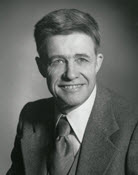
\includegraphics[scale = 1]{images/iverson.jpg}
\end{center}

\subsubsection{}

Un altro personaggio importante fu Raimondo Lullo, un filosofo, teologo e missionario catalano. Egli fu il primo a proporre un sistema di combinazione di segni per ottenere nuove conoscenze. Il suo sistema era basato su un insieme di simboli che rappresentavano le nozioni e le relazioni tra di esse. Questo sistema era chiamato \newfancyglitter{Ars Magna}.
Oltre a ciò si occupò di \newfancyglitter{logica combinatoria} nella sua opera \newfancyglitter{Ars Combinatoria}.

\section{Leibniz}

Nasce a Lipsia il 21 Giugno 1646, si laurea in Giurisprudenza nel 1666.
I suoi primi scritti sono finalizzati al conseguimento di titoli accademici. Importante in
questo periodo è la Dissertatio de Arte Combinatoria del 1666.
Negli anni immediatamente successivi alla laurea diventa consigliere dell’Elettore di
Magonza e assume diversi incarichi politici.

\begin{center}
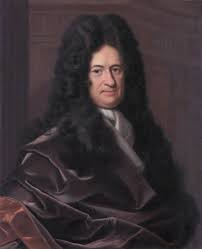
\includegraphics[scale = 0.7]{images/Leibniz.jpg}
\end{center}

Nel 1672 viene inviato a Parigi in missione diplomatica, per distogliere Luigi XIV dalla
progettata invasione dell’Olanda e invogliarlo invece alla conquista dell’Egitto.
Fallita la missione, ottiene il permesso di fermarsi a Parigi (e Londra), dove rimane per 4
anni (marzo 1672 - ottobre 1676) avendo la possibilità di conoscere la matematica e la
fisica più avanzate. Nel 1676 scopre il calcolo infinitesimale (che verrà pubblicato solo ne 1684), già
introdotto da Newton indipendentemente 10 anni prima. Nel 1705 inizierà tra i due una
polemica che finirà solo con la morte di Leibniz.
Nello stesso anno torna a Hannover come bibliotecario presso il Duca.

Tra il 1685 e il 1694: migliora la scatola di Pascal (\newfancyglitter{pascalina}) per l’addizione e la sottrazione per realizzare
anche la moltiplicazione e la divisione (e l’estrazione di radice). La macchina, che opera
mediante pulegge e ruote dentate, è conservata nella biblioteca di Hannover.

\subsection{L'origine del bit}

Leibniz fece un parallelismo tra i simboli dello yin e dello yang e i numeri binari.
Le linee piene potevano essere associate al 1, mentre le linee vuote al 0.
Così facendo si ottiene un sistema di numerazione binario.

\begin{center}
    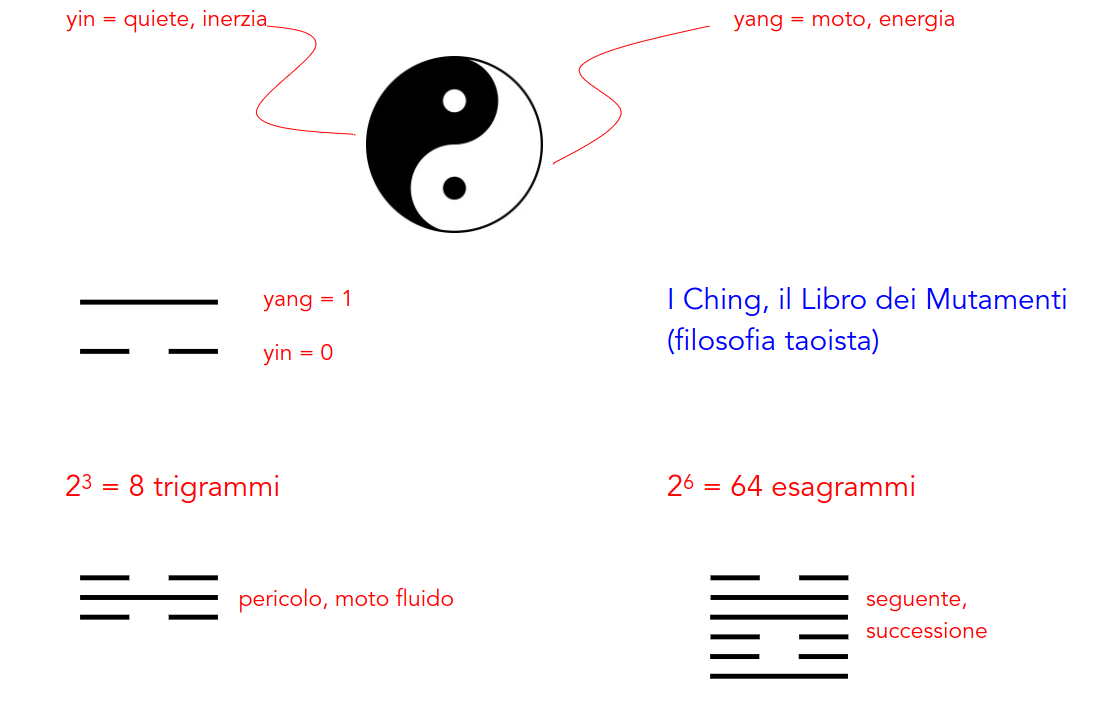
\includegraphics[scale = 0.3]{images/Origine bit.png}
\end{center}

\pagebreak

\ex{L'interpretazione di Leibniz}{
    \begin{center}
        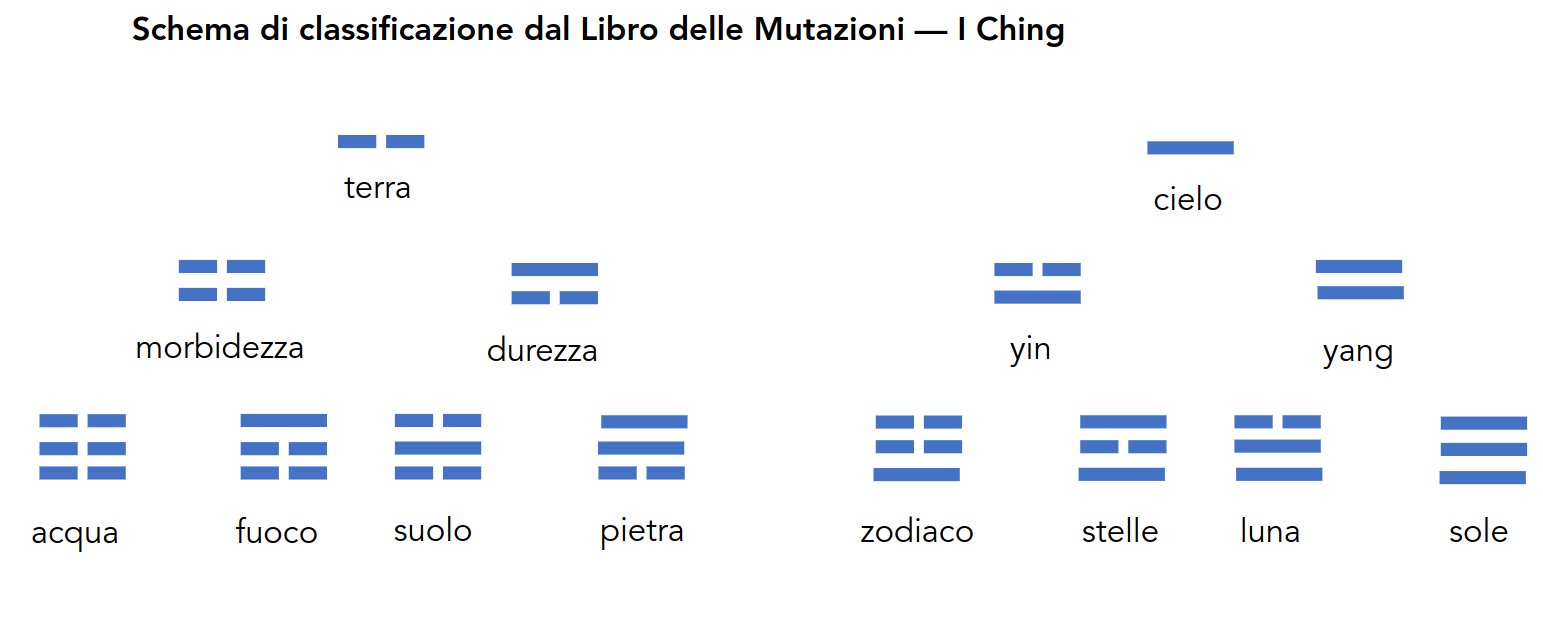
\includegraphics[scale = 0.27]{images/Bit.png}
        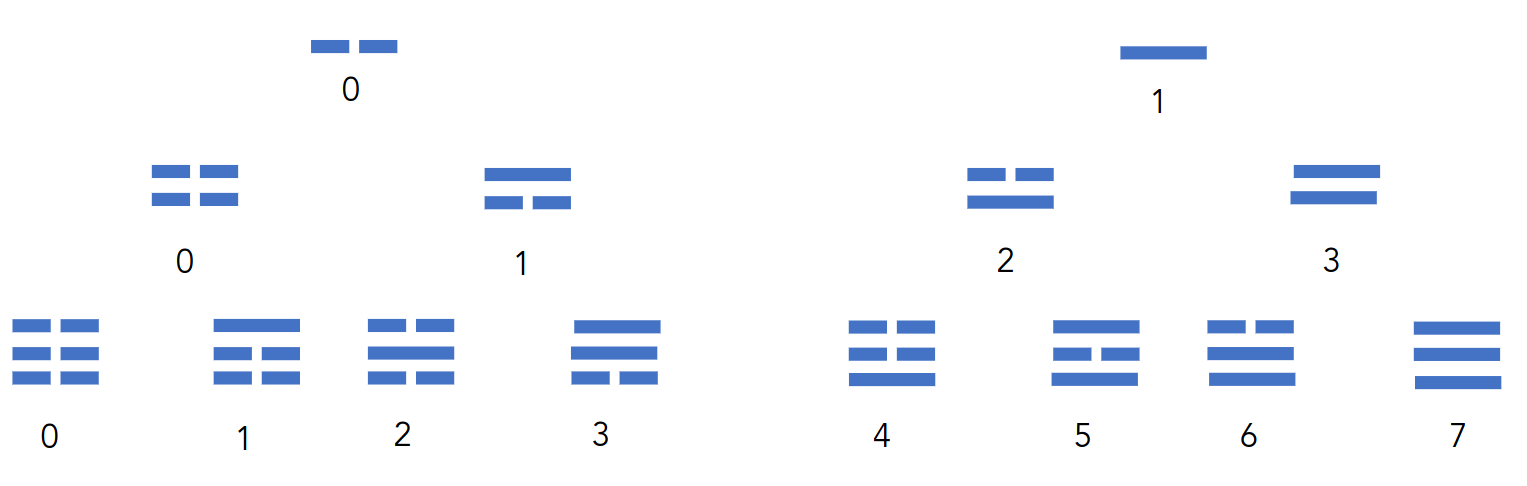
\includegraphics[scale = 0.27]{images/Associazione di Leibniz.png}
    \end{center}
}

\subsection{La caratteristica universale}

La \newfancyglitter{caratteristica universale}, concepita come lingua o scrittura universale, si fonda sui seguenti principi:

\begin{itemize}
    \item [$\Rightarrow$] Le idee sono analizzabili fino a idee semplici (atomiche);
    \item [$\Rightarrow$] Le idee possono essere rappresentate da simboli;
    \item [$\Rightarrow$] Le relazioni tra idee possono essere rappresentate da simboli;
    \item [$\Rightarrow$] Le idee si combinano mediante regole.
\end{itemize}

\dfn{Caratteristica universale}{
La \newfancyglitter{caratteristica universale}\footnote{Ispirata da Lullo e dal "Lullismo", da Atanasio Kircher e da uno scrittore anonimo del 1663.} è un sistema di segni che rappresentano
nozioni e cose, ma non parole. Le connessioni tra i segni rappresentano le relazioni tra le nozioni e le cose.
Il nome di una nozione serve a:
\begin{itemize}
    \item [$\Rightarrow$] Relazionarla con altre nozioni;
    \item [$\Rightarrow$] Relazionarla con lo schema dell'universo;
    \item [$\Rightarrow$] Indicare le esperienze necessarie per la conoscenza.
\end{itemize}
}

\nt{L'apprendimento della lingua universale coincide con l'\fancyglitter{enciclopedia}. }

\subsubsection{Il calculus ratiocinator}

\dfn{Calculus ratiocinator}{Il \newfancyglitter{calculus ratiocinator} è un insieme di tecniche per manipolare i segni della caratteristica universale. Può essere considerato come un \newfancyglitter{sistema formale}. Il frammento XX offre un'idea di questo calcolo: in esso vengono trattati molti assiomi e teoremi come il principio degli indiscernibili, la simmetria, la transitività, etc.}

\subsection{La mereologia del Frammento XX}

\dfn{Mereologia}{
    La \newfancyglitter{mereologia} è la "dottrina delle parti".
}

\dfn{Principio di identità degli indiscernibili}{
    Sono identici i termini che possono essere sostituiti a vicenda
    senza alterare la verità degli enunciati in cui compaiono. Si scrive A = B 
    quando A e B sono identici.
    \begin{itemize}
        \item [$\Rightarrow$] $B + N = L$ significa che B e N compongono L,
        cioè che B è parte di L;
        \item [$\Rightarrow$] $A\leq B$ significa che A è parte di B.
    \end{itemize}
}

\thm{Simmetria}{
    Se $A = B$ allora $B = A$.
}

\thm{Transitività}{
    Se $A = B$ e $B = C$ allora $A = C$.
}

\thm{}{
    Se $A + B = B$ allora $A \leq B$.
}

\thm{}{
    Se $A = B$ allora $A + L = B + L$.
}

\section{Ulteriori sviluppi}

\subsection{Peano e i numeri naturali}

Peano nacque a Cuneo il 27 agosto 1858. Si laureò in matematica nel 1880 e divenne professore di analisi matematica a Torino nel 1890. Nel 1889 pubblicò i suoi famosi \newfancyglitter{Principi di aritmetica}, in cui formulò un sistema assiomatico per i numeri naturali.

\begin{center}
    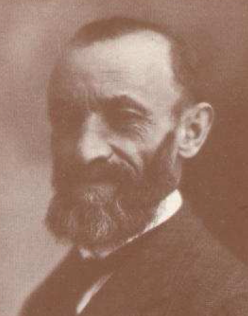
\includegraphics[scale = 0.35]{images/Peano.png}
\end{center}

\dfn{Principi di aritmetica}{
    I \newfancyglitter{Principi di aritmetica} sono un insieme
    di assiomi che definiscono i numeri naturali.
}

\subsection{Hilbert e lo Entscheidungsproblem}

Hilbert fu un matematico tedesco nato a Königsberg il 23 gennaio 1862. Egli fu uno dei più grandi matematici del XX secolo e fu uno dei fondatori della logica matematica.
Nel 1928, insieme ad Ackermann, pubblicò il libro \newfancyglitter{Grundzüge der theoretischen Logik} in cui si venne enunciato il \newfancyglitter{problema della decisione} (
    o \newfancyglitter{Entscheidungsproblem}).

\dfn{Entscheidungsproblem}{
    L'\newfancyglitter{Entscheidungsproblem} è un problema che consiste nel trovare una procedura che consente di decidere la validità di una data espressione logica con un 
    numero finito di operazioni.
}

\section{La logica matematica}

\nt{Sono trattati più in dettaglio nel corso "Metodi formali dell'Informatica" e, in
misura minore, nel corso di "Linguaggi e paradigmi di programmazione".}

\subsection{Sistemi formali}

\dfn{Sistema formale}{
    In un \newfancyglitter{sistema formale} si definiscono:
    \begin{itemize}
        \item [$\Rightarrow$] \fancyglitter{Oggetti}, che sono tutti i termini costruibili a partire 
        da atomi mediante operazioni;
        \item [$\Rightarrow$] \fancyglitter{Proposizioni}, della forma $P(a_1, ..., a_n)$ dove
        $P$ è un \fancyglitter{predicato} e $a_k$ sono termini;
        \item [$\Rightarrow$] \fancyglitter{Regole di inferenza}, che permettono di dedurre nuove proposizioni.
        La conclusione di una regola di inferenza senza premesse è un'\fancyglitter{assioma}.
    \end{itemize}

    $$\frac{A_1 \:\:\:\:\:\:\:\:\:...\:\:\:\:\:\:\:\:\: A_v}{A}$$
}

\qs{}{Come si usano le regole di inferenza?}

\paragraph{Risposta:} Per costruire derivazioni: 

\begin{figure}[h]
    \centering
    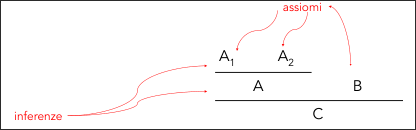
\includegraphics[scale = 0.55]{images/Inferenza.png}
    \caption{Derivazione.}
\end{figure}

\ex{Numeri naturali}{
    \begin{itemize}
        \item [$\Rightarrow$] \fancyglitter{Oggetti}: un atomo 0, un'operazione S, con un solo argomento;
        \item [$\Rightarrow$] \fancyglitter{Proposizioni}: un predicato Num con un solo argomento;
        \item [$\Rightarrow$] \fancyglitter{Regole di inferenza}: $\frac{}{\text{Num\{0\}}}$ e 
        $\frac{\text{Num\{n\}}}{\text{Num\{S(n)\}}}$.
    \end{itemize}
}

\ex{Grammatiche formali}{
    \begin{center}
        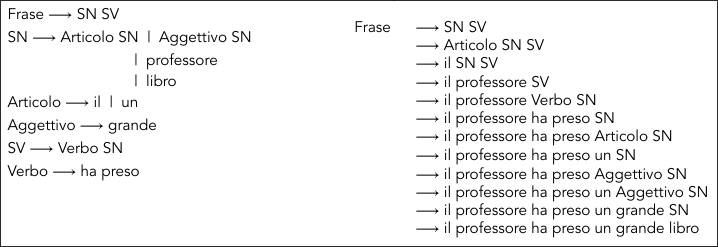
\includegraphics[scale = 0.35]{images/Gram.png}
    \end{center}
}

\subsection{Confronto tra logica e informatica}

\paragraph{Logica:}

\begin{itemize}
    \item [$\Rightarrow$] Si studiano modelli di processi deduttivi;
    \item [$\Rightarrow$] Si studiano modelli di ragionamento;
    \item [$\Rightarrow$] Operatori modali.
\end{itemize}

\paragraph{Informatica:}

\begin{itemize}
    \item [$\Rightarrow$] Si studiano modelli di processi trasformazionali;
    \item [$\Rightarrow$] Si studiano modelli di calcolo (sequenziali, paralleli, distribuiti).
\end{itemize}


\subsection{Kleene e le funzioni ricorsive}

Nel 1981 Stephen Cole Kleene, matematico e logico statunitense,
pubblicò l'articolo "\fancyglitter{Origins of recursive function theory}" in cui
descrisse l'attività di ricerca svolta da alcuni matematici
e logici negli anni '30. In particolare, Kleene descrisse
una serie di lezioni di G\"odel tenute nel 1934 a Princeton
sullo sviluppo di definizioni ricorsive primitive di funzioni 
numeriche. Lo \fancyglitter{schema di ricorsione primitiva} permette di
definire una funzione di numeri naturali f(\textbf{x}, n) a partire da funzioni 
predefinite b(\textbf{x}) e h(\textbf{x}, n, m) mediante lo schema:

$$f(x, 0) = b(x)$$

$$f(x, n + 1) = h(x, n , f(x, n))$$
\subsubsection*{}
Inoltre si ha la composizione:

$$f(x) = h(g_1(x), \cdot\cdot\cdot, g_k(x))$$

\subsubsection*{}

G\"odel usava la nozione di \newfancyglitter{sistema matematico formale} basata
sulla nozione informale di \newfancyglitter{regola costruttiva} la cui
applicazione si basava su una \newfancyglitter{procedura finita} del tipo
necessario per calcolare funzioni definite mediante ricorsioni generali.
\subsubsection{}
Nasce il problema della caratterizzazione delle ricorsioni ammissibili.
Kleene aggiunse un \fancyglitter{operatore di ricerca} non limitato
che dato un predicato P(x, y) restituisce il valore minimo che soddisfa
il predicato. 
Nel 1938, Kleene ammise la possibilità di definire funzioni
parziali.

\section{Curry e la logica combinatoria}

Nel 1927, Haskell Brooks Curry, matematico e logico statunitense,
riscopri la nozione di \fancyglitter{combinatore} (introdotta da
Moses Sch\"onfinkel nel 1920).

\dfn{Combinatore}{
    Un \newfancyglitter{combinatore} è una funzione senza variabili libere.
}

\nt{I sistemi di combinatori attuali usano K e S come combinatori,
perché sono sufficienti a generare tutti gli altri combinatori.}

\ex{Combinatori}{
    \begin{itemize}
        \item [$\Rightarrow$] K(x, y) = x;
        \item [$\Rightarrow$] S(x, y, z) = x(z)(y(z)).;
        \item [$\Rightarrow$] B(x, y, z) = x(y(z));
        \item [$\Rightarrow$] C(x, y, z) = x(z)(y);
        \item [$\Rightarrow$] W(x, y) = x(y)(y).
        \item [$\Rightarrow$] I(x) = x.
    \end{itemize}
}

\subsubsection*{}

Inoltre riprende anche la possibilità di trattare funzioni a più argomenti
come funzioni a un solo argomento che verrà chiamata \newfancyglitter{curryficazione}.

$$f(x, y) = f'(x)(y)$$

\subsubsection*{}

Nello stesso tempo, Alonzo Church, sviluppa il \newfancyglitter{lambda calcolo}\footnote{Visto approfonditamente nei corsi 
"Metodi formali dell'informatica" e "Linguaggi e paradigmi di programmazione, per cui in questi appunti non andrò
in dettaglio dato che esula gli obiettivi del corso.}.

\dfn{Lambda calcolo}{
    Il \newfancyglitter{lambda calcolo} è un sistema formale per la definizione di funzioni
    intese come regole di corrispondenza. $\lambda x.M$ descrive la regola che assegna
    a un argomento $x$ il valore $M$.
}

\subsection{Paradosso di Russell e combinatori}

$$WS(BWB) = Y = \lambda x.(\lambda z.x(zz)) (\lambda z.x(zz))$$

\nt{Si tratta del combinatore di punto fisso.
Permette di definire funzioni ricorsive.}

\dfn{Paradosso di Russell}{

    $$(\lambda x.(\lambda z.x(zz)) (\lambda z.x(zz))) \neg = 
     (\lambda z.\neg(zz)) (\lambda z.\neg(zz))$$

    In cui $\{z | \neg (z \in z)\} \in \{z | \neg (z \in z)\}$.
    Ciò vuol dire che qualcosa appartiene a se stesso, ma
    non può appartenere a se stesso.

}

\section{L'analisi dei processi di calcolo di Turing}

Nel paragrafo 9 del suo articolo del 1936, Turing introduce
il comportamento di un \fancyglitter{computor}. Lo esemplifica con un
foglio di carta che viene astratto come un "nastro infinito" suddiviso in
caselle (quadratini):
\begin{itemize}
    \item [$\Rightarrow$] Il numero di simboli che si possono stampare è finito,
    perché se ci fossero infiniti simboli ci si potrebbe confondere\footnote{Un po'
    come il fatto che molti caratteri Unicode non possono essere usati nei
    nomi dei siti web in quanto troppo "simili".};
    \item [$\Rightarrow$] Il comportamento è determinato dallo stato mentale
    e dal simbolo osservato, c'è un limite alla percezione delle caselle per lo stesso
    motivo di prima;
    \item [$\Rightarrow$] Le operazioni sono elementari, cioè non possono essere
    ulteriormente scomposte. Esse consistono in cambiamenti di stato mentale e  
    del simbolo osservato\footnote{Un solo simbolo viene alterato.}.
\end{itemize}

\begin{figure}[h]
    \centering
    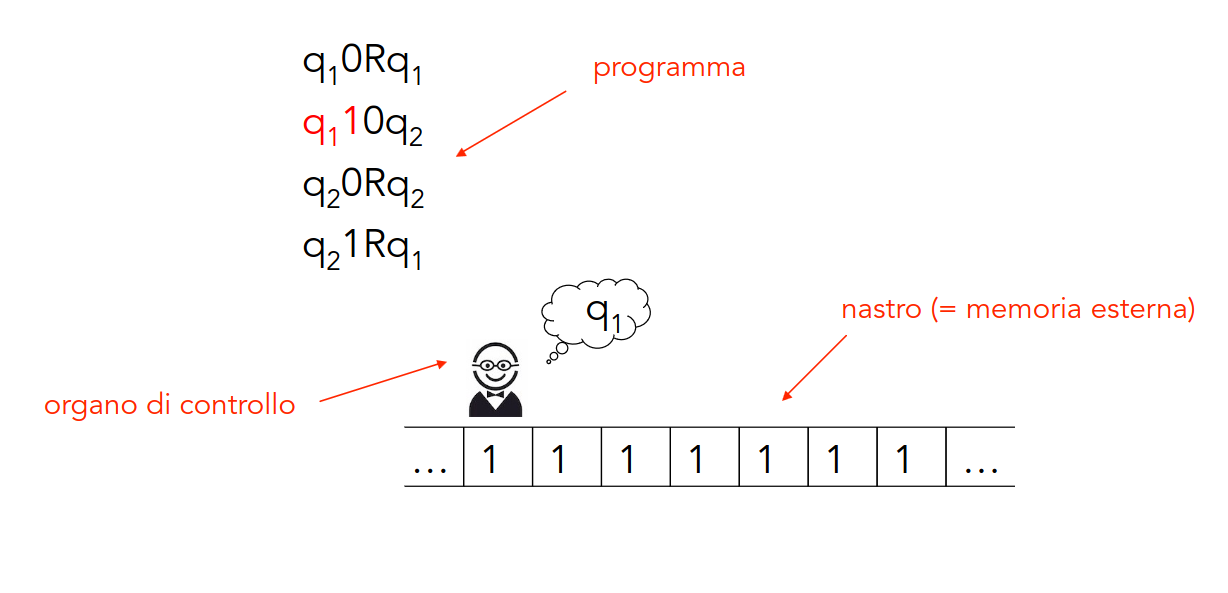
\includegraphics[scale = 0.35]{images/Turing.png}
    \caption{Macchine di Turing come Computer.}
\end{figure}

\dfn{Macchina universale}{
    Una \newfancyglitter{macchina universale} ($U$) è una macchina di Turing
    che può simulare il comportamento di qualsiasi altra macchina di Turing ($M$)
    dato il suo programma ($I_M$) per ogni dato $x$:

    $$U(I_M, x) = M(x)$$

    È possibile che $U$ sia più complessa di $M$. In informatica, il
    programma di $U$ è chiamato \newfancyglitter{interprete}. 

    }

    \nt{Questo risultato suggerirà a von Neumann la possibilità di
    automi che generano automi di pari o maggiore complessità.}


\subsection{Non tutte le funzioni sono calcolabili da una macchina di Turing}

Per dimostare che non tutte le funzioni sono calcolabili da una macchina di Turing  si può
utilizzare la \fancyglitter{diagonalizzazione di Cantor}\footnote{Visto nel corso "Matematica discreta".}:
\begin{itemize}
    \item [$\Rightarrow$] Si immagina di poter numerare le funzioni da $\bbN$ in $\bbN$;
    \item [$\Rightarrow$] Si considera una funzione da $\bbN$ in $\{0,1\}^\bbN$;
    \item [$\Rightarrow$] Questo elenco può essere visto come una tabella;
    \item [$\Rightarrow$] Si vuole dimostrare che esiste una sequenza che non è in questa tabella;
    \item [$\Rightarrow$] Si prende la diagonale, che interseca tutte le righe in un punto;
    \item [$\Rightarrow$] Si cambiano tutti i valori della diagonale (0 diventa 1 e viceversa);
    \item [$\Rightarrow$] La diagonale trasformata può essere una riga dell'originale?
    \item [$\Rightarrow$] No, perché differisce da ogni riga in almeno un punto.
\end{itemize}

\begin{figure}[h]
    \centering
    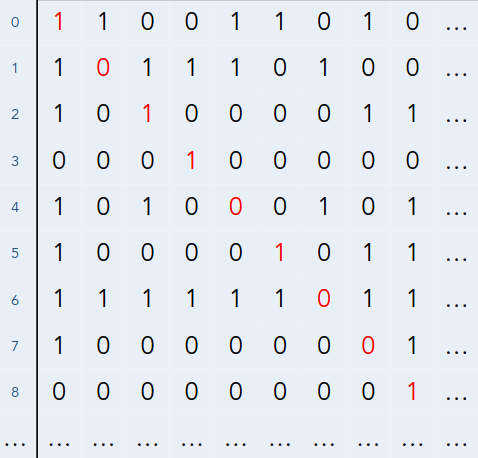
\includegraphics[scale = 0.38]{images/Diagonalizzazione.png}
    \caption{Diagonalizzazione di Cantor.}
\end{figure}

\begin{figure}[h]
    \centering
    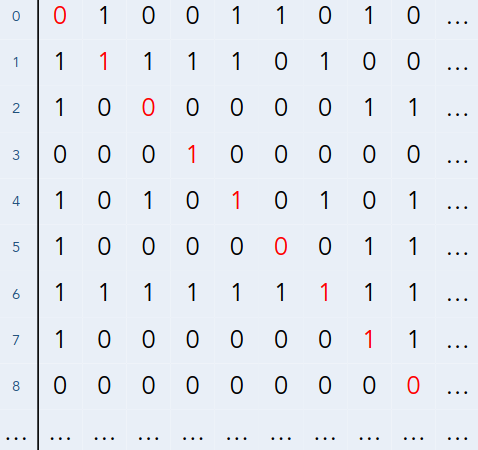
\includegraphics[scale = 0.38]{images/Diagonalizzazione 2.png}
    \caption{Diagonalizzazione di Cantor, inversione della diagonale.}
\end{figure}

\cor{Problemi indecidibili}{
    Non esiste una macchina di Turing $M$ che, operando su un nastro che contiene:
    \begin{itemize}
        \item [$\Rightarrow$] La descrizione di una qualsiasi macchina di Turing $T$;
        \item [$\Rightarrow$] Un input $x$.
    \end{itemize}
    termina sempre i suoi calcoli scrivendo sul nastro il valore $M(T, x)$ dove:
    \begin{itemize}
        \item [$\Rightarrow$] $M(T, x) = 1$ se $T(x)$ termina;
        \item [$\Rightarrow$] $M(T, x) = 0$ se $T(x)$ non termina.
    \end{itemize}
}
\nt{Il problema della fermata è indecidibile.}

\section{Von Neumann: il Computer come Organismo Artificiale}

Von Neumann, matematico e fisico ungherese\footnote{Già visto
nella prima parte del corso.}, fu influenzato dalle idee di
McCulloch e Pitts\footnote{
    \textit{A logical calculus of the ideas immanent in nervous activity}.
}, che avevano definito un modello di neurone
le cui reti potevano essere caratterizzate come \fancyglitter{automi finiti}\footnote{Notato da Kleene nel 1951}.

\begin{figure}[h]
    \centering
    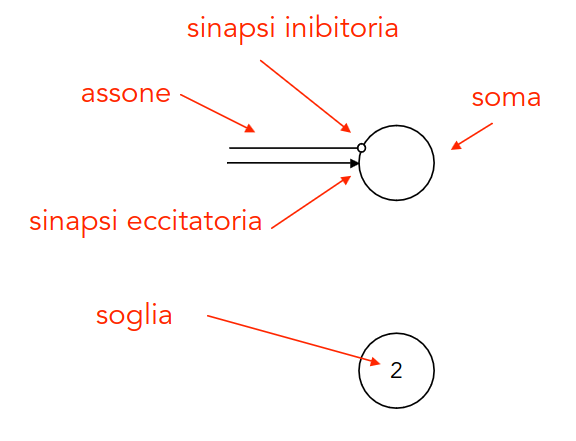
\includegraphics[scale = 0.25]{images/McCulloch-Pitts.png}
    \caption{Il neurone di McCulloch e Pitts.}
\end{figure}

\subsubsection{}

Nel 1945, von Neumann pubblicò il "First Draft of a Report on the EDVAC" in cui
descriveva gli elementi di un calcolatore in termini "biologici" utilizzando
il modello di McCulloch e Pitts:

\begin{itemize}
    \item [$\Rightarrow$] \fancyglitter{CPU}: neuroni di associazione;
    \item [$\Rightarrow$] \fancyglitter{Input}: neuroni sensoriali;
    \item [$\Rightarrow$] \fancyglitter{Output}: neuroni motori.
\end{itemize}

\subsubsection{}

L'obiettivo di von Neumann era quello di \fancyglitter{unificare}, tramite una
teoria generale degli automi, il lavoro di Turing sulle macchine teoriche,
il lavoro di McCulloch e Pitts sui neuroni e il lavoro di Shannon sulla
teoria dell'informazione\footnote{Si vedrà nel prossimo capitolo.}.

\nt{Questo tentativo verrà criticato dai neurofisiologi perché
tentava di descrivere computer e cervello assiomatizzando il comportamento
di \fancyglitter{scatole nere}.}

\subsection{Automi cellulari}

Negli anni '40, a Los Alamos, von Neumann e Ulam ebbero l'idea di
automi che operino su una griglia di celle infinita (bidirezionale).
Ogni cella ha un proprio stato e lo stato di una cella in un'istante $T$
dipende dallo stato delle celle adiacenti in un istante $T - 1$. Il modello
di von Neumann e Ulam aveva 29 stati.

\clm{}{}{
    Da notare che la nozione di \fancyglitter{celle adiacenti} è relativa:
    per von Neumann erano solo 4 (nord, sud, est, ovest), mentre per Moore
    erano 8 (aggiungeva anche le diagonali). Oltre a questo esistono altri modelli con
    celle esagonali e con forme diverse.
}

\begin{figure}[h]
    \centering
    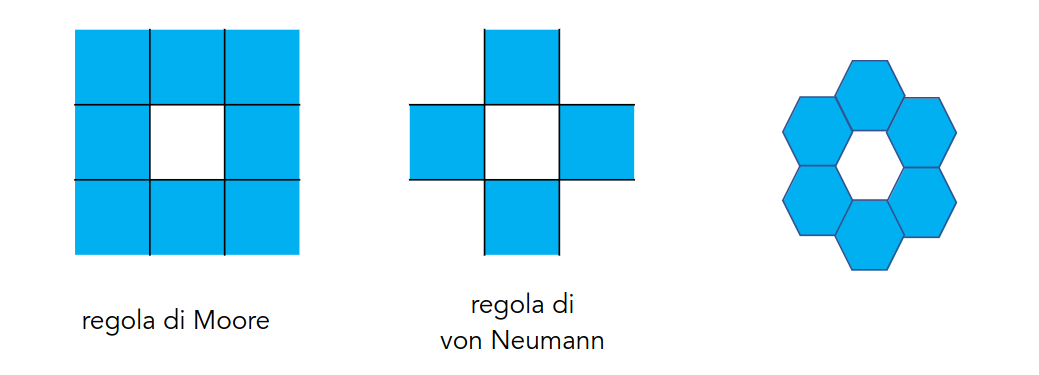
\includegraphics[scale = 0.3]{images/Automi cellulari.png}
    \caption{Ci sono differenti versioni.}
\end{figure}

\paragraph{Per von Neumann c'erano due modi di descrivere gli automi cellulari:}

\begin{itemize}
    \item [$\Rightarrow$] \fancyglitter{McCulloch-Pitts (modo sintetico)}: strutture
    costruite a partire da elementi più semplici. Bisogna solo definire gli elementi e le loro connessioni (può essere complesso);
    \item [$\Rightarrow$] \fancyglitter{Turing (modo integrale)}: si descrive, tramite assiomi, l'intero automa senza descrivere
    gli elementi da cui è composto, ma solo il loro comportamento.
\end{itemize}

\begin{figure}[h]
    \centering
    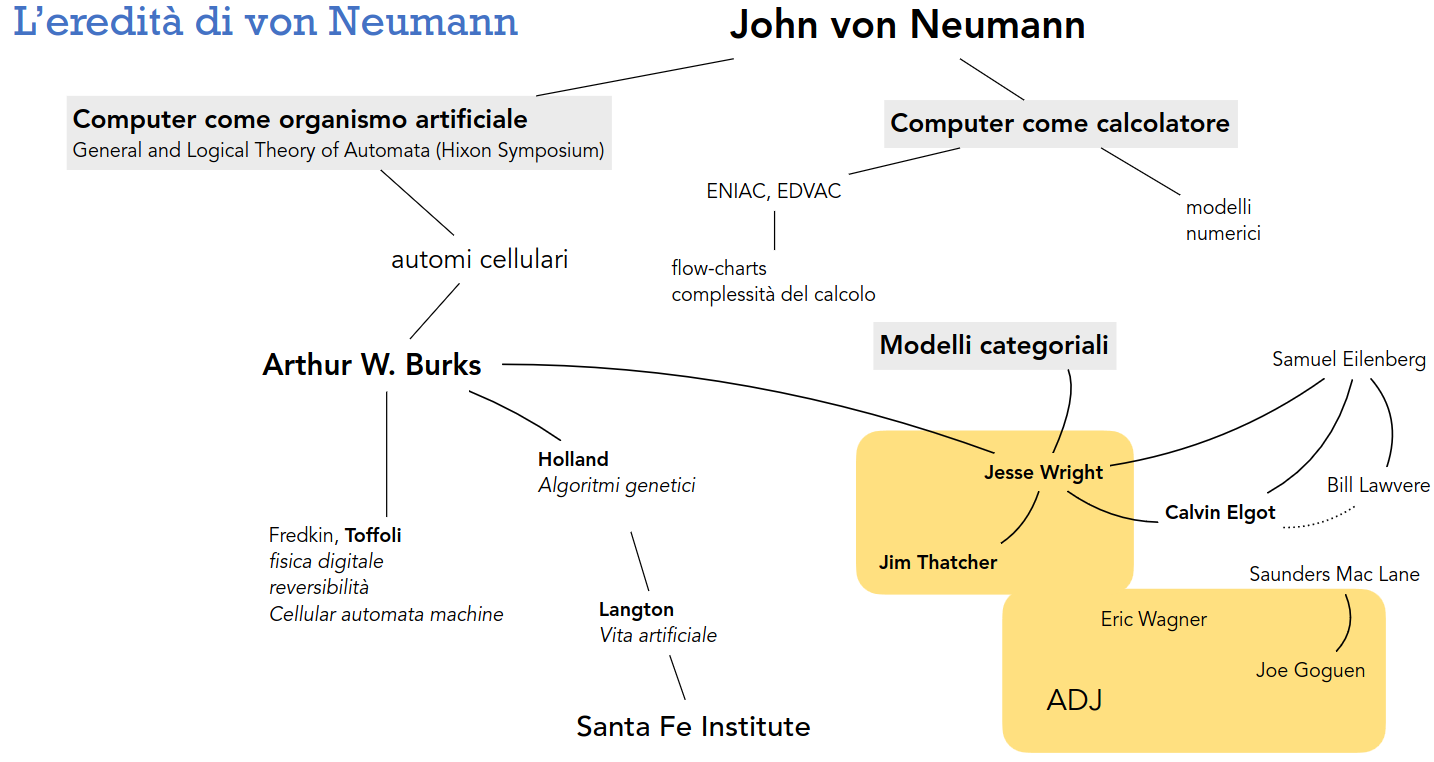
\includegraphics[scale = 0.33]{images/V1.png}
    \caption{Sommario.}
\end{figure}

\subsection{La Vita Artificiale secondo Conway (Game of Life)}

\dfn{Game of Life}{
    Il \newfancyglitter{Game of Life} è un automa cellulare ideato da John Conway nel 1970.
    Si basa su una griglia bidimensionale di celle quadrate, ognuna delle quali può essere
    in uno di due stati: vivo o morto. Le celle comunicano con le otto celle adiacenti.
    È un gioco a zero giocatori, cioè il suo sviluppo è determinato solo dallo stato iniziale.
}

\cor{Regole}{
    Le regole sono le seguenti:
    \begin{itemize}
        \item [$\Rightarrow$] Una cella morta con esattamente tre celle vive adiacenti diventa viva;
        \item [$\Rightarrow$] Una cella viva con due o tre celle vive adiacenti rimane viva;
        \item [$\Rightarrow$] In tutti gli altri casi la cella muore.
    \end{itemize}
}

\begin{figure}[h]
    \centering
    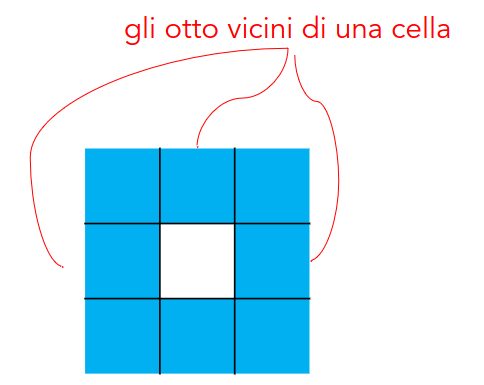
\includegraphics[scale = 0.3]{images/Conway.png}
    \caption{Game of Life.}
\end{figure}

\nt{Una configurazione famosa è il \fancyglitter{glider} (aliante), che si muove
nella griglia.}

\begin{figure}[h]
    \centering
    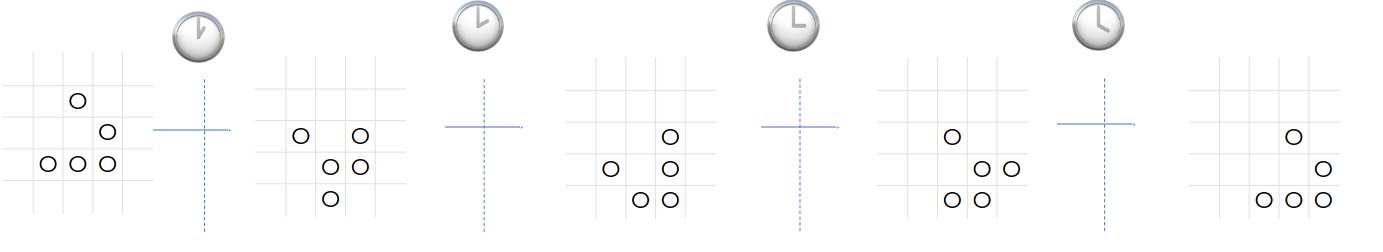
\includegraphics[scale = 0.3]{images/Glider.png}
    \caption{Glider.}
\end{figure}


%%%%%%%%%%%%%%%%%%%%%%%%%%%%%%%%%
% Informazione e cibernetica
%%%%%%%%%%%%%%%%%%%%%%%%%%%%%%%%%

\definecolor{chaptergrey}{rgb}{0,0,0.7}

\ifnum\layout=2 
    \fancyhf{}      
    \renewcommand{\headrulewidth}{0pt}
    \renewcommand{\chaptermark}[1]{\markboth{#1}{}}

    \fancyhead[LE]{\nouppercase{\textbf{\textcolor{chaptergrey}{\chaptername}}~ \thechapter~ |~ \leftmark}}
    \fancyhead[RO]{\nouppercase{ \rightmark}}
    \fancyfoot[LE,RO]{\thepage}
    \fancypagestyle{plain}{         
    \fancyhf{}
    \fancyfoot[LE,RO]{\thepage}}    
 \else          
    \renewcommand{\headrulewidth}{0pt}
    \fancyhf{}                  
    \fancyhead[C]{\nouppercase{ \leftmark}}
    \fancyfoot[C]{\thepage}
\fi

\chapter{Informazione e cibernetica}

\section{Shannon}

Claude Shannon fu un matematico che lavorò per la Bell Labs.  Nel 1948 scrisse un articolo,
\fancyglitter{A Mathematical Theory of Communication}, in cui ha definito la teoria dell'informazione\footnote{Nella laurea magistrale è presente il corso "Teoria dell'Informazione" che approfondice questi argomenti.}: 
"il problema fondamentale della comunicazione è quello di 
riprodurre ad un punto, esattamente o con qualche approssimazione, un messaggio
scelto in un altro punto".

\paragraph{Shannon definisce un contesto tecnico di termini:}
\begin{itemize}
    \item [$\Rightarrow$] \fancyglitter{Emittente - Ricevente}: il mittente è colui che invia il messaggio, il ricevente è colui che lo riceve.
    \item [$\Rightarrow$] \fancyglitter{Messaggio}: è l'informazione che si vuole trasmettere.
    \item [$\Rightarrow$] \fancyglitter{Rumore}: è tutto ciò che può interferire con la trasmissione del messaggio.
    \item [$\Rightarrow$] \fancyglitter{Informazione}: è la quantità di incertezza che si riduce nel ricevente dopo aver ricevuto il messaggio.
\end{itemize}


\nt{L'informazione in  sé è considerata in base al numero di possibili 
messaggi che possono essere inviati.}

\begin{figure}[h]
    \centering
    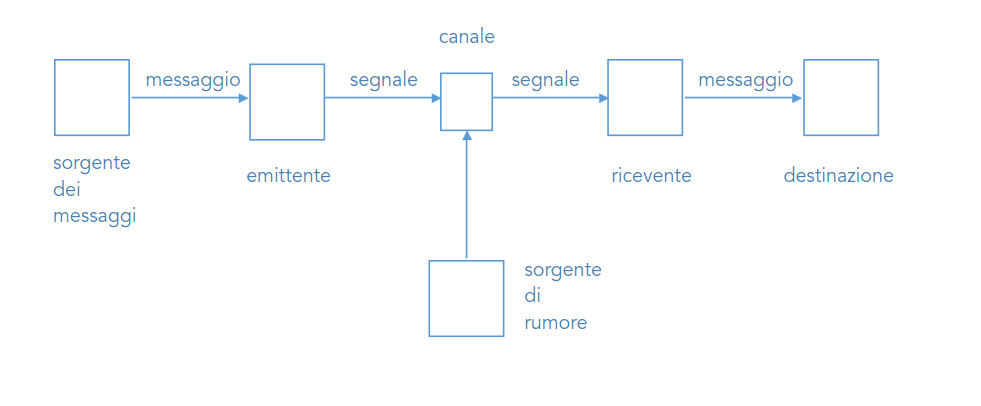
\includegraphics[scale=0.35]{images/Shannon.png}
    \caption{Schema di Shannon}
\end{figure}

\clm{}{}{
    L'informatica non è solamente uno scheletro che può essere riempito con
    qualsiasi cosa. Alla sua base vi sono idee e atteggiamenti fondanti che
    possono essere applicati in molti campi. Un esempio è la cibernetica che ha 
    avuto una breve durata (circa 20 anni), ma ha avuto un impatto molto forte
    in molte aree della scienza e della tecnologia.

    Esiste un'epistemologia dell'informatica, che ne studia
    le basi e le fondamenta. 
    
    Se si vuole approfondire l'argomento, nella prima parte del corso
    "Metodologie e Tecnologie Didattiche dell'Informatica" (MTDI o PREFIT)
    si ha una panoramica "motivazionale" sulle basi dell'informatica e sul suo
    essere una scienza.    
}

\subsection{Il modello di comunicazione}

Il modello di comunicazione di Shannon purtroppo non mette in evidenza
il fattore temporale e il ritardo. Quando si comunica in un contesto asincrono
bisogna utilizzare un sistema di feedback per capire se il messaggio è stato
ricevuto correttamente\footnote{Per esempio il sistema di ACK (Acknowledgement) di TCP
visto nel corso "Reti I"/"Reti di calcolatori".}. Il modello di comunicazione di Shannon
ha avuto varie interpretazioni, una delle quali è quella di Chapman.

\begin{figure}[h]
    \centering
    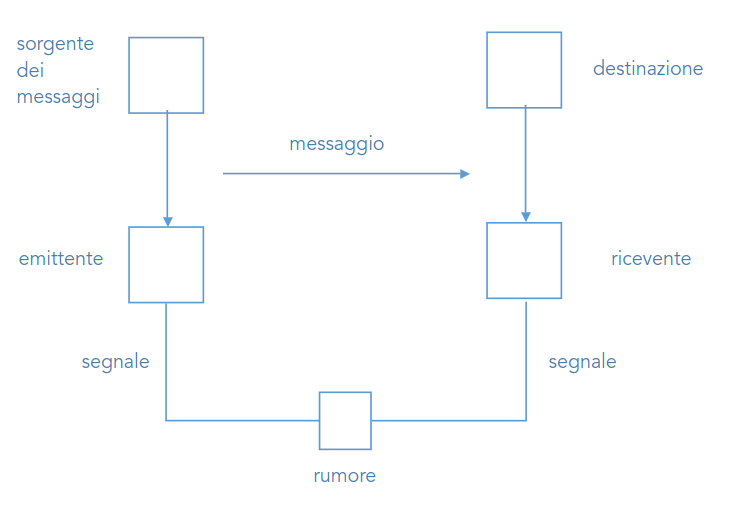
\includegraphics[scale=0.35]{images/Chapman.png}
    \caption{Modello di comunicazione di Shannon, reinterpretato da Chapman.}
\end{figure}

\paragraph{In questa interpretazione vengono identificati i livelli a cui i segnali possono esistere:}
\begin{itemize}
    \item [$\Rightarrow$] Nello strato basso è presente il rumore;
    \item [$\Rightarrow$] Al livello superiore è presente il messaggio.
\end{itemize}

\section{Nascita della cibernetica}

\subsection{Cibernetica e neurofisiologia}

La cibernetica viene codificata da Norbert Wiener nel 1948, e si occupa di studiare i sistemi di controllo e di comunicazione nei sistemi biologici 
e nelle macchine.
Von Neumann aveva come obiettivo l'unificazione del lavoro di McCulloch e Pitts con il lavoro di Shannon e di Turing. Per Wiener,
la nozione unificante era il feedback, mentre per von Neumann era la nozione di automa come
elaboratore di informazione.

\subsubsection{Lavori di von Neumann sugli automi:}

\begin{itemize}
    \item [$\Rightarrow$] \fancyglitter{The general and logical theory of automata}, Hixon Symposium, 1948;
    \item [$\Rightarrow$] \fancyglitter{Theory and organization of complicated automata}, serie di 5 lezioni all'università dello Illinois, 1949;
    \item [$\Rightarrow$] \fancyglitter{Probabilistic logics and the synthesis of reliable organisms from unreliable components}, appunti delle lezioni alla Caltech, 1952;
    \item [$\Rightarrow$] \fancyglitter{The Theory of Automata: Construction, Reproduction, Homogeneity}, 1952-1953;
    \item [$\Rightarrow$] \fancyglitter{The computer and the brain}, Yale University Press, 1956 pubblicato postumo.
\end{itemize}

\subsubsection{}

\paragraph{Per ricapitolare le relazioni tra i vari "attori":}

\begin{itemize}
    \item [$\Rightarrow$] \fancyglitter{Shannon - Turing}: si incontrano nel 1943 ai Bell Labs, e discutono di comunicazione\footnote{Da ricordare Enigma e la crittografia.};
    \item [$\Rightarrow$] \fancyglitter{Wiener - Von Neumann - McCulloch - Pitts}: partecipano alle conferenze di Macy la cui nozione centrale è il messaggio (con le accezioni di Shannon);
    \item [$\Rightarrow$] \fancyglitter{Wiener - McCulloch - Pitts}: membri del RLE;
    \item [$\Rightarrow$] \fancyglitter{Von Neumann - Turing}: si incontrano nel 1937 a Princeton. Nel 1939 von Neumann offre a Turing un posto di lavoro come assistente a Princeton, ma Turing rifiuta;
    \item [$\Rightarrow$] \fancyglitter{Shannon - Wiener}: sviluppano una teoria matematica e della comunicazione basata sulla concezione dell'informazione/entropia di un insieme di messaggi.
\end{itemize}

\clm{}{}{Pare che Shannon adorasse il monociclo e che spesso tenesse dei party
in cui si esibiva in numeri di equilibrismo.
}

\begin{figure}[h]
    \centering
    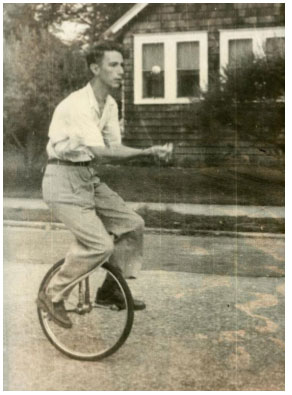
\includegraphics[scale=0.30]{images/Shannon monocycle.jpg}
    \caption{Shannon sul monociclo}
\end{figure}

\subsection{Von Neumann e la termodinamica del calcolo}

Von Neumann cercò di valutare il costo energetico minimo per un
atto elementare di generazione di informazioni. Da ciò deriva, nel 1949,
la formula:

$$kT \log_e N$$

\begin{itemize}
    \item [$\Rightarrow$] $k$: costante di Boltzmann;
    \item [$\Rightarrow$] $T$: temperatura;
    \item [$\Rightarrow$] $N$: numero di alternative o possibili stati.
\end{itemize}
\subsubsection{}
Questo calcolo attirò le attenzioni di \fancyglitter{Landauer}, un fisico teorico, 
che non riuscì a dimostrarlo, ma osservò che le operazioni logicamente
irreversibili (come l'operazione di cancellazione di un bit) generano entropia
pari alla quantità di informazione cancellata. \fancyglitter{Bennet}, un suo studente,
nel 1973, dimostrò che ogni calcolo può essere reso logicamente reversibile.
\fancyglitter{Fredkin}, un altro fisico teorico, 
lavorò a una base fisica per i calcoli reversibili.

\nt{Da questo tipo di interessi nasce la computazione quantistica (
    che cosa succede se si considera la computazione come composta da operazioni
    meccaniche?).}

\begin{figure}[h]
    \centering
    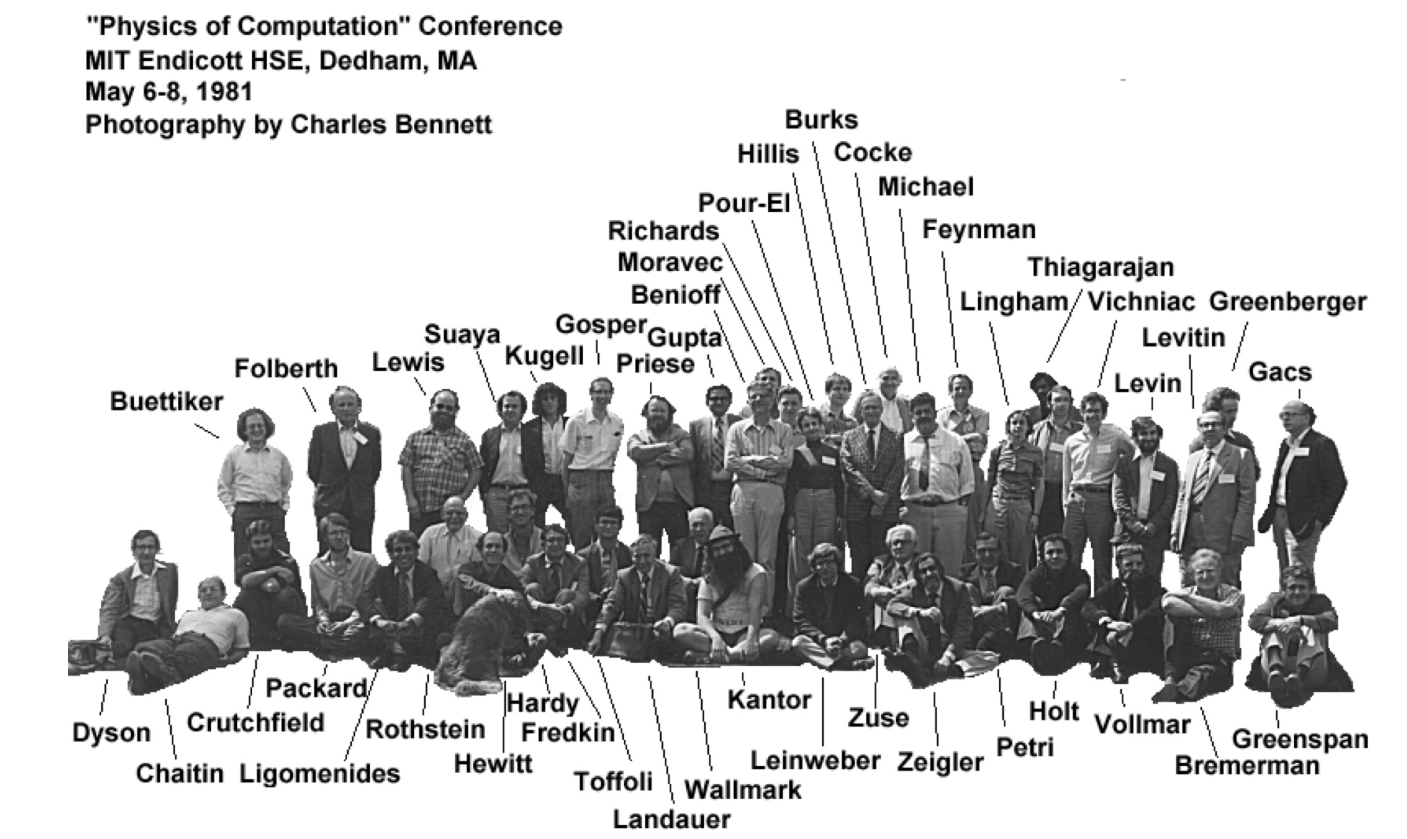
\includegraphics[scale=0.3]{images/Comp.png}
    \caption{Physics of Computation}
\end{figure}

\clm{}{}{
    \begin{itemize}
        \item [$\Rightarrow$] \fancyglitter{Bennet}: è un fisico teorico, non è direttamente
        presente nella foto perché fu lui a scattarla;
        \item [$\Rightarrow$] \fancyglitter{Landauer}: è presente nella foto in primo piano;
        \item [$\Rightarrow$] \fancyglitter{Fredkin}: è presente nella foto, vicino a Landauer e Toffoli;
        \item  [$\Rightarrow$] \fancyglitter{Toffoli}: fu uno studioso di fisica della computazione che interagi con
        Burks;
        \item  [$\Rightarrow$] \fancyglitter{Burks}: in secondo piano;
        \item [$\Rightarrow$] \fancyglitter{Feynman}, \fancyglitter{Dysan} e altri fisici famosi;
        \item [$\Rightarrow$] \fancyglitter{Zuse}: già visto nella prima parte del corso, inventore dello Z1;
        \item [$\Rightarrow$] \fancyglitter{Kantor}: inventore e specialista dell'informazione come principio ontologico;
        \item [$\Rightarrow$] \fancyglitter{Holt}: esperto di cibernetica;
        \item [$\Rightarrow$] \fancyglitter{Gosper}: inventore della configurazione ad aliante, uno dei primi "hacker".
    \end{itemize}
}

\section{La cibernetica}

Quando si \fancyglitter{comunica} con un'altra persona le si trasmette un
messaggio, e quando l'altra persona risponde, si riceve un messaggio che contiene
informazioni accessibili a sé stessi e all'altro. Ma anche quando si \fancyglitter{controllano}
le azioni di un'altra persona le si comunica un messaggio (in forma imperativa). 
Tutto ciò si riduce a uno \fancyglitter{scambio di messaggi}.

\dfn{Cibernetica}{
    La \newfancyglitter{cibernetica} può essere vista come una teoria della
    trasmissione dei messaggi e delle sue condizioni che presentano un successo.
}

\nt{Il computer diventa un oggetto cibernetico, in quanto è inserito in un
contesto di comunicazione con esseri umani o con altri computer.}

\subsection{Il feedback e il flusso di messaggi}
\label{feedback}
Wiener confrontava l'attività umana con quella di figure che danzano sopra
un carillon secondo un modello. Tuttavia il modello in esame è un modello
predisposto in cui il loro passato non ha influenza sul loro futuro. Non 
c'è feedback.

\begin{figure}[h]
    \centering
    
\includegraphics[scale=0.35]{images/IO.png}
    \caption{Modello IO}
\end{figure}

\subsubsection{}

Holt propose l'idea che quando una persona scrive su una macchina premendo il tasto
esso fornisce un feedback tornando indietro. La temporizzazione dei tasti è
ciò che consente la scrittura.
Questo si può estendere all'utente e all'interfaccia: la scelta di un'interfaccia comporta
la progettazione dell'utente indicando cosa si può o non si può fare.

\ex{Scatola nera}{
    Si immagini una scatola con dei pulsanti che si possono premere. Quando si preme un pulsante
    si accende una luce. Prima di poter schiacciare un altro pulsante bisogna controllare che la luce
    si sia accesa. In questo caso la luce è il feedback.
    \begin{center}
        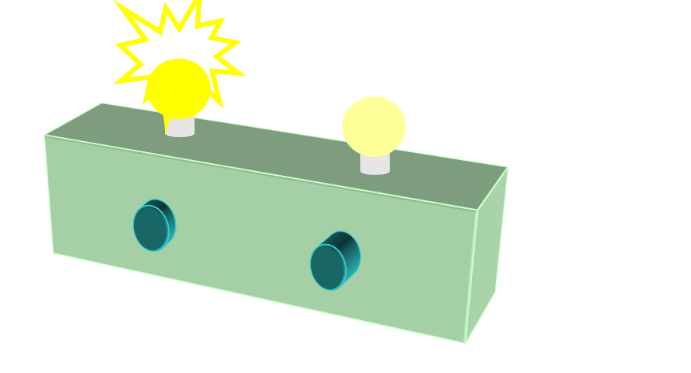
\includegraphics[scale=0.35]{images/Scatola nera.png}
    \end{center}

    Se i pulsanti sono premuti da un operatore che non può vedere le luci e 
    le luci sono visibili a un altro operatore che non può premere i pulsanti,
    non si potrebbe stabilire una corrispondenza tra luci e pulsanti e dunque la connessione non ha 
    succeso.

    \begin{center}
        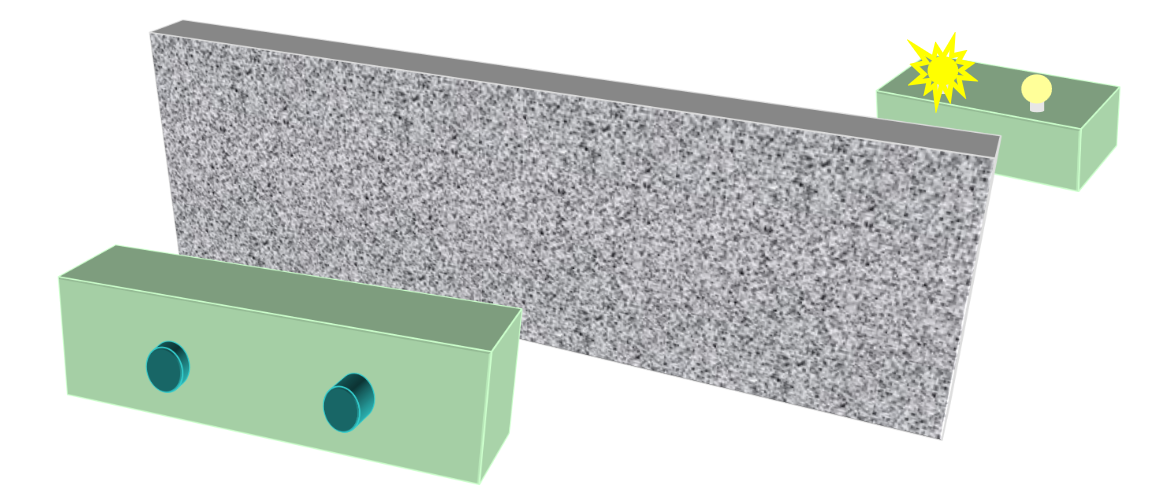
\includegraphics[scale=0.35]{images/Scatola nera 2.png}
    \end{center}

}

\subsection{Osservatori}

In alcuni sistemi, per esempio un termostato, è l'osservatore a concettualizzare il ciclo.
Nei sistemi di secondo ordine, l'osservatore è esso stesso parte del sistema osservato.

\begin{figure}[h]
    \centering
    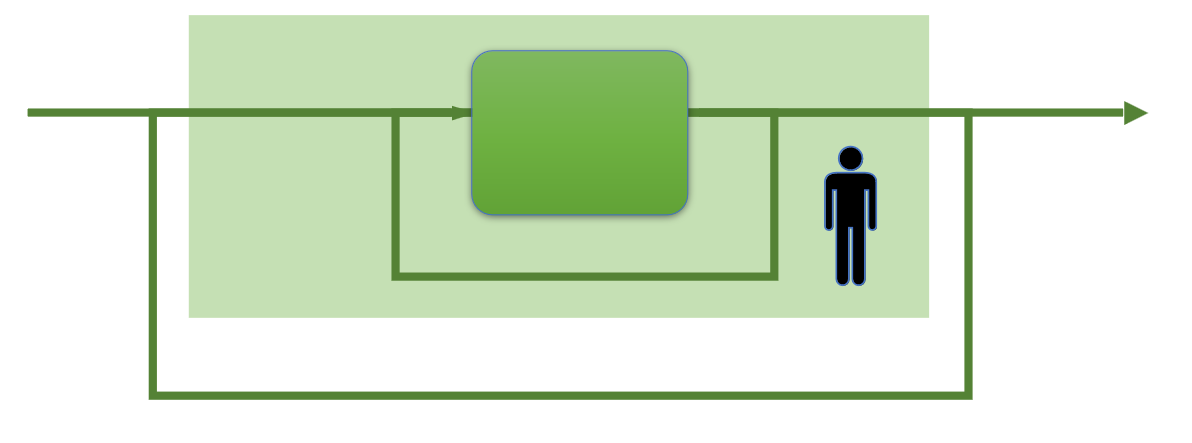
\includegraphics[scale=0.25]{images/Osservatore.png}
    \caption{Osservatore}
\end{figure}

\subsection{Comunicazione sincrona e asincrona}

\dfn{Comunicazione sincrona}{
    La \newfancyglitter{comunicazione sincrona} è una comunicazione in cui il mittente e il ricevente
    sono sincronizzati. 
    
    In una comunicazione sincrona è presente un unico sistema di riferimento
    temporale condiviso da tutti i partecipanti. 

}

\ex{Comunicazione sincrona}{
    \begin{itemize}
        \item [$\Rightarrow$] Chiamata telefonica;
        \item [$\Rightarrow$] Conversazione faccia a faccia;
        \item [$\Rightarrow$] Sistema di posta elettronica in cui i messaggi impiegano $n$ secondi per 
        essere consegnati;
        \item [$\Rightarrow$] Segnali di fumo.
    \end{itemize}
}

\dfn{Comunicazione asincrona}{
    La \newfancyglitter{comunicazione asincrona} è una comunicazione in cui il mittente e il ricevente
    non sono sincronizzati. 
    
    In una comunicazione asincrona non è presente un unico sistema di riferimento
    temporale condiviso da tutti i partecipanti. 

}

\ex{Comunicazione asincrona}{
    \begin{itemize}
        \item [$\Rightarrow$] Sistema di posta elettronica con garanzia di consegna entro $n$ secondi;
        \item [$\Rightarrow$] Sistema postale ordinario;
        \item [$\Rightarrow$] Messaggi in bottiglia.
    \end{itemize}
}

\nt{Nella comunicazione asincrona è necessario un sistema di feedback per capire se il messaggio è stato ricevuto.}

\dfn{Circuiti asincroni}{
    I \newfancyglitter{circuiti asincroni} sono circuiti in cui i segnali di controllo
    non sono sincronizzati con un segnale di clock (orologio globale).
}

\cor{C-Muller}{
    Un elemento asincrono è il C-Muller per cui l'uscita è 1 se e solo se
    entrambi gli ingressi sono 1 e diventa 0 se entrambi gli ingressi sono 0.
}

\begin{figure}[h]
    \centering
    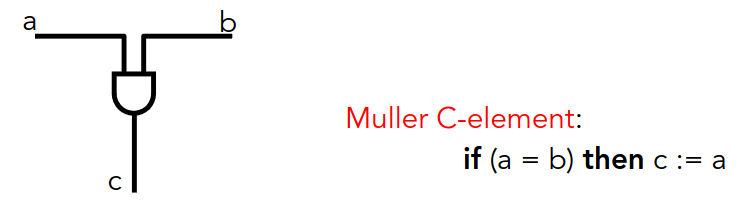
\includegraphics[scale=0.33]{images/C-Muller.png}
    \caption{C-Muller}  
\end{figure}

\nt{Combinando più C-Muller si può costruire un circuito asincrono che implementa
le micropipeline.}

\begin{figure}[h]
    \centering
    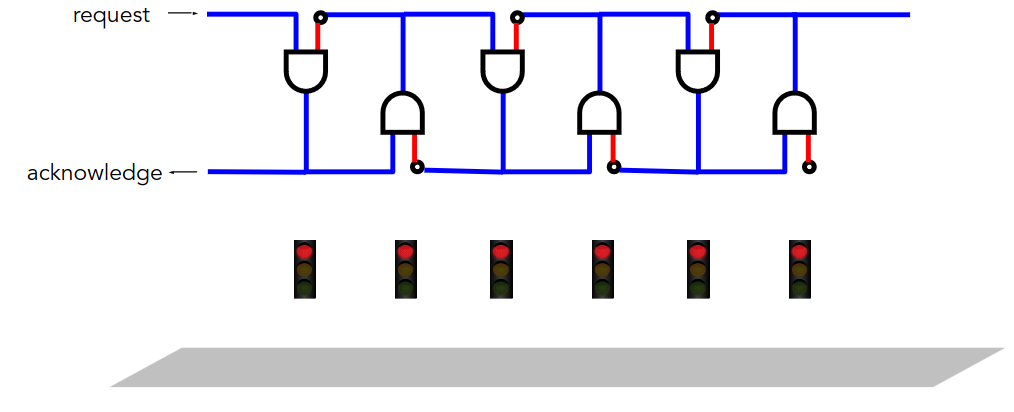
\includegraphics[scale=0.25]{images/Micropipeline.png}
    \caption{Micropipeline}
\end{figure}

\cor{Reti di Petri}{
    Grafi che generalizzano gli automi a stati finiti (DFA e NFA).
    Si hanno posti (condizioni) e transizioni (eventi).
}

\begin{figure}[h]
    \centering
    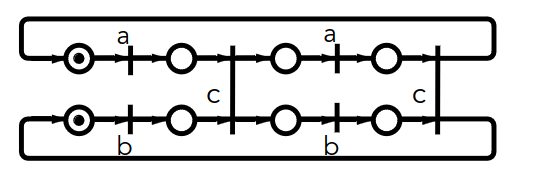
\includegraphics[scale=0.35]{images/Petri.png}
    \caption{Rete di Petri}
\end{figure}












%%%%%%%%%%%%%%%%%%%%%%%%%%%%%%%%%
% Bush ed Engelbart
%%%%%%%%%%%%%%%%%%%%%%%%%%%%%%%%%

\definecolor{chaptergrey}{rgb}{1,0.75,0}

\ifnum\layout=2 
    \fancyhf{}      
    \renewcommand{\headrulewidth}{0pt}
    \renewcommand{\chaptermark}[1]{\markboth{#1}{}}

    \fancyhead[LE]{\nouppercase{\textbf{\textcolor{chaptergrey}{\chaptername}}~ \thechapter~ |~ \leftmark}}
    \fancyhead[RO]{\nouppercase{ \rightmark}}
    \fancyfoot[LE,RO]{\thepage}
    \fancypagestyle{plain}{         
    \fancyhf{}
    \fancyfoot[LE,RO]{\thepage}}    
 \else          
    \renewcommand{\headrulewidth}{0pt}
    \fancyhf{}                  
    \fancyhead[C]{\nouppercase{ \leftmark}}
    \fancyfoot[C]{\thepage}
\fi

\chapter{Bush ed Engelbart, Memex e Demo}

\section{Introduzione}

\dfn{Knowledge Navigator}{
    Un'idea di Apple (John Sculley), presentata nel 1987, di un assistente virtuale
    che aiuta l'utente a navigare tra le informazioni.
}

\subsubsection{Il filmato di presentazione del Knowledge Navigator (1987):}

\begin{itemize}
    \item [$\Rightarrow$] \fancyglitter{La comprensione del parlato}:
    il computer capisce il linguaggio naturale;
    \item [$\Rightarrow$] \fancyglitter{La grafica e le finestre}:
    dietro questo video c'è Alan Kay, che ha lavorato a Xerox PARC e fu 
    l'inventore delle finestre;
    \item [$\Rightarrow$] \fancyglitter{Il touch screen};
    \item [$\Rightarrow$] \fancyglitter{La videochiamata};
    \item [$\Rightarrow$] \fancyglitter{La simulazione}: della desertificazione.
\end{itemize}

\qs{}{Chi era Vannevar Bush?}

\paragraph{Risposta:} Vannevar Bush (1890 - 1974) fu un ingegnere e scienziato americano.
Bush teorizzò il Memex
(non fu mai realizzato).

\nt{Durante una conferenza in occasione del 50° anniversario di "As 
we may think" (1945) venne presentata un'animazione del Memex.}
\pagebreak
\section{Il Memex}

\dfn{Memex}{
    Un sistema di archiviazione e ricerca delle informazioni, teorizzato da Vannevar Bush.
}

\nt{Il Memex offre anche un'anticipazione di ciò che sarà l'\fancyglitter{
    ipertesto} (Ted Nelson), che nascerà vent'anni dopo.
}

\subsection{Problemi di organizzazione dell'informazione}

Il problema che preoccupava Bush era \fancyglitter{la perdita di informazioni} che si accumulano
continuamente nel tempo\footnote{Questo problema non era nuovo. 
Era già stato affrontato da Paul Otlet.}. Inoltre la specializzazione tende ad aumentare progressivamente: 
le informazioni sono sempre più frammentate e sempre più
specializzate (più difficili da comunicare). Bush riteneva che il problema 
non fosse l'eccesso di pubblicazioni, ma il fatto che si fossero estese oltre
la capacità di gestione dei documenti. 

\nt{La \fancyglitter{selezione}\footnote{Processo di scelta delle informazioni.}
è un problema per via delle enormi quantità di informazioni.}

\ex{Addetto dell'ufficio informazioni}{
    L’addetto all’ufficio del personale di una fabbrica immette una pila di alcune migliaia di schede
degli impiegati in una macchina selezionatrice, imposta un codice secondo una convenzione
stabilita e produce in poco tempo una lista di tutti gli impiegati che vivono a Trenton e
conoscono lo spagnolo.
}

\ex{Centralini telefonici automatici}{
    Si compone un
numero e la macchina seleziona e connette solamente una tra un milione di possibili stazioni.
Non le ispeziona tutte. Presta attenzione solo a una classe data dalla prima cifra, poi solo a una
sottoclasse data dalla seconda cifra e così via; così procede rapidamente e quasi infallibilmente
verso la stazione selezionata.
}

\paragraph{Prroblemi dell'indicizzazione:}

\begin{itemize}
    \item [$\Rightarrow$] Si cerca da sottoclasse a sottoclasse;
    \item [$\Rightarrow$] L'informazione si trova in un unico punto (a meno che non sia duplicata);
    \item [$\Rightarrow$] Bisogna avere regole per specificare il percorso, ma le regole sono complicate;
    \item [$\Rightarrow$] Quando si trova l'elemento bisogna riemergere dal sistema e rientrare attraverso un nuovo percorso.
\end{itemize}

\nt{La situazione peggiore, ma più facilmente verificabile, è la ricerca in un albero.}

\dfn{Classificazione}{
    La \newfancyglitter{classificazione} è una segmentazione spaziale, temporale o spazio-temporale del mondo.
    
    Un sistema di classificazione è un insieme di scatole in cui si mettono cose per fare un 
    qualche tipo di lavoro.
}

\paragraph{Proprietà di un sistema di classificazione:}

\begin{itemize}
    \item [$\Rightarrow$] Ci sono principi univoci e consistenti;
    \item [$\Rightarrow$] Le categorie sono reciprocamente esclusive;
    \item [$\Rightarrow$] Il sistema è completo.
\end{itemize}

\begin{figure}[h]
    \centering
    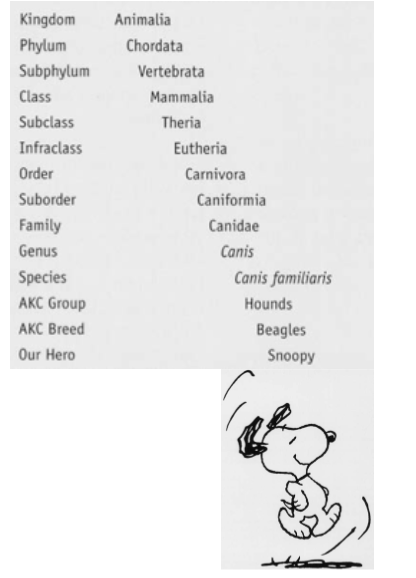
\includegraphics[scale=0.5]{images/Snoopy.png}
    \caption{Snoopy secondo due sistemi di classificazione.}
\end{figure}

\subsection{Indicizzazione}

\dfn{Indicizzazione}{
    L'operazione di \newfancyglitter{indicizzazione} è l'azione di descrivere o identificare
    un documento (o un oggetto) nei termini del suo contenuto concettuale\footnote{ISO 5963.}.
}

\nt{Lo scopo generale dell'indicizzazione è quello di rappresentare oggetti
in modo che possano essere efficacemente trovati e utilizzati.}

\cor{Linguaggio di indicizzazione}{
    Un linguaggio di indicizzazione è un sistema di rappresentazioni simboliche (un codice)
    che consentono la classificazione e la ricerca di documenti attraverso
    i codici assegnati ai concetti che essi contengono (indicizzazione per concetti).
}

\nt{Ted Nelson, in "As we will think", criticherà il fraintendimento
per cui si vede nel lavoro di Bush un contributo alla information retrieval\footnote{Reperimento di oggetti informativi.}.
}


\subsection{Browser vs Search}

Le seguenti definizioni sono state date da Clay Shirky in "Ontology is Overrated. 
Categories, Links, and Tags" (2005).

\dfn{Browse}{
    \newfancyglitter{Browse} significa che le persone fanno ontologia
    e categorizzazione, avendo la responsabilità di organizzare il mondo in anticipo.
}

\nt{Il browse è uno schema passivo.}

\dfn{Ricerca}{
    Il paradigma della \newfancyglitter{ricerca} sostiene che nessuno può
    prevedere cosa sarà necessario in futuro. Quando se ne ha bisogno si tenterà
    di trovarlo basandosi sulla struttura di link disponibile.
}

\nt{Per esempio, Google è un sistema di ricerca.}

\begin{figure}[h]
    \centering
    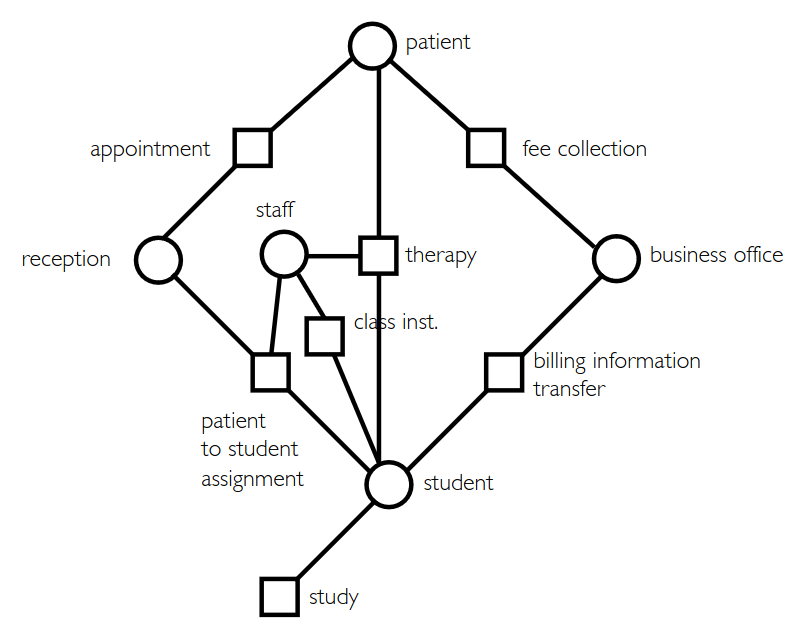
\includegraphics[scale=0.5]{images/UniBoston.png}
    \caption{Il sistema di classificazione della scuola dentistica dell'Università di Boston - Ruoli e attività.}
\end{figure}

\begin{figure}
    \centering
    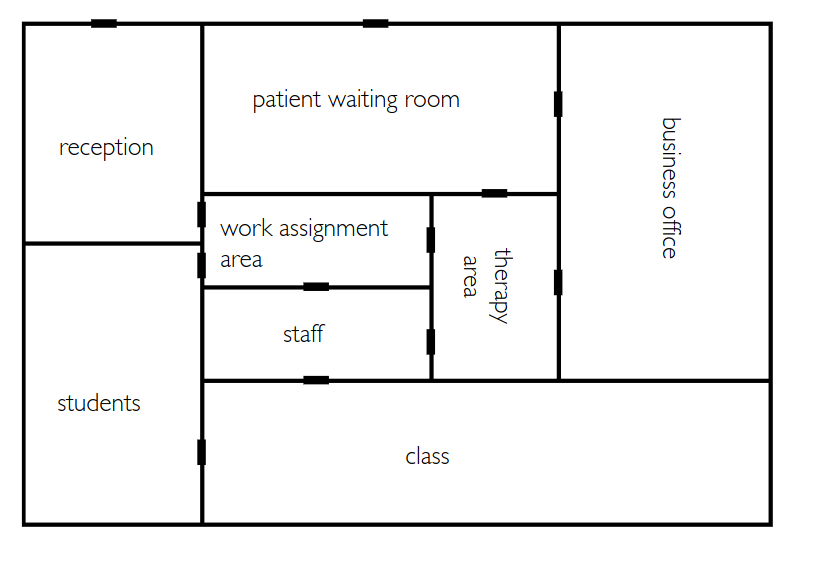
\includegraphics[scale=0.4]{images/UniBoston2.png}
    \caption{Il sistema di classificazione della scuola dentistica dell'Università di Boston - Mappa degli spazi.}
\end{figure}

\nt{Un esempio di gerarchia ad albero si ha nel filesystem del Multics.}

\begin{figure}[h]
    \centering
    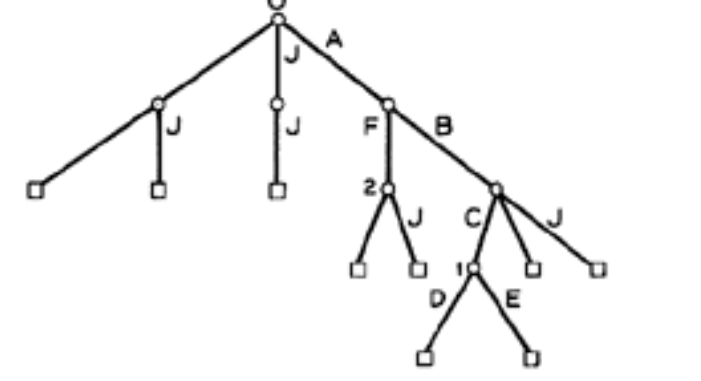
\includegraphics[scale=0.25]{images/Unix.png}
    \caption{Filesystem Multics.}
\end{figure}


\subsection{Associazione}

La mente umana, secondo Bush, lavora per associazione: quando 
"afferra" un elemento scatta istantanemente a quello successivo in base 
a un'associazione di pensieri in accordo con una rete di percorsi determinata dai neuroni.
La selezione per associazione può essere meccanizzata dal \fancyglitter{Memex}.
Nel Memex vengono archiviati tutti i libri, le registrazioni e le comunicazioni.
Esso è meccanizzato in modo da essere consultato con estrema velocità e flessibilità.
Si tratta di un supplemento \fancyglitter{personalizzato} e allargato alla memoria dell'individuo.

\paragraph{Il Memex è uno strumento \textit{personale}:}

\begin{itemize}
    \item [$\Rightarrow$] È utilizzato da una sola persona;
    \item [$\Rightarrow$] L'utilizzatore lo adatta ai propri interessi;
    \item [$\Rightarrow$] Il Memex non è collegato ad altri dispositivi (non esiste una rete di Memex).
\end{itemize}

\nt{Il Memex è stato disegnato da Alfred D. Crimi, in Life.}

\clm{}{}{
    La versione del Memex su Life (As we may think) è stata letta da Engelbart in una 
    baracca della croce rossa nelle Filippine. Engelbart rievocherà
    questa descrizione tra la fine degli anni '50 e l'inizio degli anni '60
    quando deciderà di dedicarsi ad alcune problematiche di cui aveva avuto
    un'anticipazione nell'articolo di Bush (questo porterà a nLS e alla Demo).
}

\subsection{Le funzionalità del Memex}

La maggior parte dei contenuti del Memex è archiviata su microfilm (con rapid selector).
Il microfilm è un grande limite del Memex, in quanto analogico.

\paragraph{Le potenzialità del collegare elementi:}

\begin{itemize}
    \item [$\Rightarrow$] Fornisce un passo verso un'\fancyglitter{indicizzazione associativa}\footnote{Qualsiasi elemento può immediatamente selezionarne automaticamente un altro.};
    \item [$\Rightarrow$] Quando un utente crea un percorso, il Memex lo \fancyglitter{nomina},
    \fancyglitter{inserisce il nome nel libro dei codici} e lo batte sulla tastiera;
    \item [$\Rightarrow$] In fondo a ogni elemento ci sono degli \fancyglitter{spazi vuoti} per immettere dei codici e viene impostato un puntatore per indicarne uno per ciascun elemento;
    \item [$\Rightarrow$] L'utente preme un singolo tasto e gli elementi vengono uniti in modo permanente\footnote{Nei relativi spazi appare il codice.}.
\end{itemize}

\subsubsection{}
Questo processo fa si che, in qualsiasi momento, quando uno di questi elementi
viene richiamato, venga richiamato anche l'altro\footnote{Proprio come un ipertesto.}.
Si può dire che gli oggetti fisici siano stati raccolti da fonti remote e rilegati
insieme per \fancyglitter{formare un nuovo libro}\footnote{
    Quest'idea (un libro costruito attivamente da chi lo sta consultando), anticipata da Otlet,
    verrà ripresa da Licklider a proposito delle \fancyglitter{biblioteche del futuro}.
}.


\ex{Un Caso d'Uso del Memex}{
    \subsubsection{Questo esempio è ripreso parola per parola dalle slides del prof. Cardone.}

    Poniamo il caso che il proprietario del memex sia interessato all’origine e alle proprietà dell’arco
e delle frecce. Più precisamente egli sta studiando la ragione per cui l’arco corto turco fu
apparentemente migliore dell’arco lungo inglese nei combattimenti delle Crociate.

Egli ha dozzine di libri e articoli potenzialmente pertinenti nel suo memex.

Prima sfoglia un’enciclopedia, trova un articolo interessante ma non abbastanza dettagliato, e lo
lascia proiettato. Poi, in un libro di storia, trova un altro articolo pertinente e collega i due
insieme. Procede in questo modo, creando un percorso composto da molti elementi.

Occasionalmente inserisce un proprio commento, collegandolo al percorso principale o,
attraverso un percorso laterale, a uno specifico elemento.

Quando diventa evidente che le proprietà di elasticità dei materiali a disposizione avevano
molto a che fare con l’arco, egli crea una ramificazione su un percorso laterale che lo porta a testi
sull’elasticità e a tabelle di costanti fisiche.

Egli inserisce una pagina di analisi scritta a mano da lui stesso.

Quindi crea un percorso di suo interesse attraverso il labirinto dei materiali a sua disposizione.
Diversi anni più tardi [c]on un tocco accede al libro dei codici. Premendo alcuni tasti egli proietta
l’inizio del percorso. Con una leva lo scorre a piacere fermandosi sugli elementi interessanti,
facendo delle digressioni.

Appariranno tipi totalmente nuovi di enciclopedie, già munite di una rete di tracce associative
che le attraversano, pronte per essere immesse nel memex dove vengono ampliate. [Esempi
sull’uso di una grande massa di informazioni da parte di avvocati, medici e scienziati.]

Lo storico con un vasto resoconto cronologico di un popolo lo accosta ad un percorso saltuario
che si sofferma solamente sui temi salienti, e può seguire in ogni momento percorsi paralleli che
lo portano a spaccati di civiltà in particolari epoche.

}

\clm{}{}{
    Wikipedia è nata in un'ottica di collegamenti e di ipertesti. 
    Il concetto di \fancyglitter{wiki}, inventato da Ward Cunningham, fu implementato per la prima volta in \fancyglitter{HyperCard}.
    Inoltre Cunningham è anche noto in ambito di programmazione OO per l'Extreme Programming (XP), visto nel corso 
    "Sviluppo Applicazioni Software".
}

\dfn{Apripista}{
    Un'\newfancyglitter{apripista} è una nuova professione che si occupa di
    stabilire \newfancyglitter{percorsi utili} attraverso l'enorme massa delle informazioni
    archiviate.
}

\section{Il progetto di Doug Engelbart: Demo}

\begin{itemize}
    \item [$\Rightarrow$] 1945: Legge "As we may think" di Vannevar Bush;
    \item [$\Rightarrow$] 1957: Entra alla Stanford Research Institute (SRI);
    \item [$\Rightarrow$] 1962: Pubblica il rapporto "Augmenting Human Intellect: A Conceptual Framework";
    \item [$\Rightarrow$] 1963: partono i finanziamenti per il progetto allo "Augmentation Research Center" (ARC)
    \footnote{Anche grazie a Licklider.};
    \item [$\Rightarrow$] 1968: La "madre di tutte le dimostrazioni" (Demo), San Francisco;
    \item [$\Rightarrow$] 1969: Primo collegamento ARPANET\footnote{Uno dei primi nodi a essere associati ad ARPANET fu proprio quello del SRI.} (tra UCLA e ARP).
\end{itemize}

\dfn{Augmenting Human Intellect}{
    \newfancyglitter{Augmenting Human Intellect} (il rapporto del 1962) contiene la proposta
    del progetto e \newfancyglitter{anticipa} tutte le realizzazioni tecnologiche fino al 1968.
    Esso punta a migliorare l'efficacia intellettuale dell'uomo, scivolando nell'interazione/simbiosi tra uomo e macchina.
}

\clm{}{}{
    A un certo punto del progetto si fece uso di uno strumento hardware a 5 dita e gli operatori
    comunicavano tra loro, da una postazione all'altra, mostrando le dita della mano.
}

\subsection{L'idea di "Augmentation"}

Engelbart puntava ad affrontare i problemi "\fancyglitter{complessi}": di diplomatici,
di scienziati, di fisici, avvocati, etc.. Questi problemi vanno affrontati 
non tramite trucchetti, ma comprendendo il problema. I problemi possono 
essere ben posti/tame problems o mal posti/wicked problems (sul lato della progettazione\footnote{
    Un esempio è la pianificazione di una linea di metropolitana. I problemi
    urbanistici sono generalmente wicked problems.
}).

\begin{figure}[h]
    \centering
    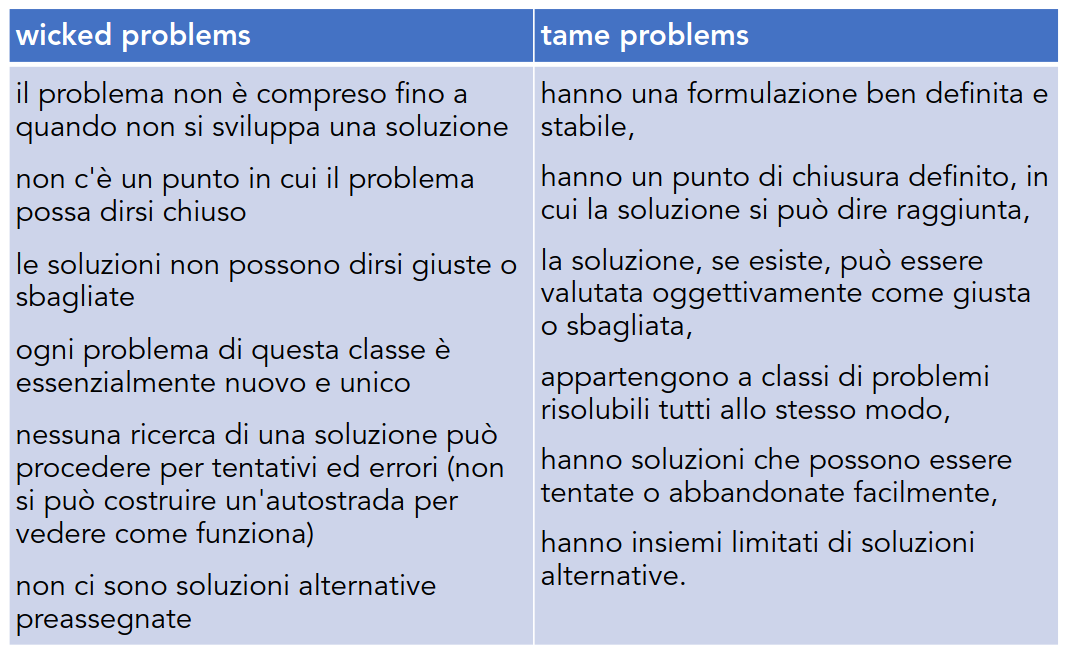
\includegraphics[scale=0.32]{images/Problems.png}
    \caption{Problemi mal posti vs. Problemi ben posti.}
\end{figure}

\nt{La questione dei problemi mal posti e ben posti è affrontata 
approfonditamente nel corso "Metodologie e Tecnologie Didattiche per l'Informatica".}
\pagebreak
\ex{Quali wicked e quali tame?}{
    Con \textcolor{red}{\XSolidBrush} si indicano i wicked problems e con \textcolor{green}{\Checkmark} i tame problems.

    \begin{itemize}
        \item [\textcolor{green}{\Checkmark}] Trovare la radice quadrata di 7358.
        \item [\textcolor{green}{\Checkmark}] Trovare il cammino più breve tra un punto A e un punto B.
        \item [\textcolor{red}{\XSolidBrush}] Progettare un'automobile sicura.
        \item [\textcolor{green}{\Checkmark}] Riparare una lavatrice.
        \item [\textcolor{red}{\XSolidBrush}] Costruire una linea di metropolitana.
        \item [\textcolor{green}{\Checkmark}] Racimolare 10.000 euro.
        \item [\textcolor{red}{\XSolidBrush}] Organizzare una mostra.
        \item [\textcolor{red}{\XSolidBrush}] Preparare un disegno di legge.
    \end{itemize}


}

\ex{Un architetto "aumentato"}{
    Engelbart racconta l'esempio di un architetto che sta progettando un edificio.

    \paragraph{Attività di questo architetto aumentato da un computer (il "\fancyglitter{clerk}"):}
    \begin{itemize}
        \item [$\Rightarrow$] Ha già fantasticato su diverse strutture e le \fancyglitter{mette alla prova sullo schermo};
        \item [$\Rightarrow$] Sullo schermo ha una \fancyglitter{vista prospettica} del sito di costruzione sul 
        pendio della collina sormontata dalla sede stradale, una rappresentazione dei vari alberi che devono rimanere
        sul terrebìno e i vari punti di allacciamento per i servizi;
        \item [$\Rightarrow$] Con il \fancyglitter{puntatore} indica due punti di interesse;
        \item [$\Rightarrow$] Dopo un po' l'architetto \fancyglitter{cambia la scena} sullo schermo in una visione dall'alto che mostra lo scavo;
        \item [$\Rightarrow$] \fancyglitter{Immette con la tastiera un elenco di elementi} controllandoli uno a uno mentre appaiono sullo schermo, rimandandone lo studio in seguito.
    \end{itemize}


}

\subsection{Classi di Strumenti di Aumentazione}
\label{augmentation}
\begin{itemize}
    \item [$\Rightarrow$] \fancyglitter{Artefatti}: oggetti fisici progettati per la comodità dell'uomo,
    per la manipolazione di cose, materiali e simboli.
    \item [$\Rightarrow$] \fancyglitter{Linguaggio}: i modi in cui l'individuo segmenta l'immagine del 
    mondo in concetti che la sua mente usa per modellare, i simboli che associa a 
    quei concetti e utilizza nella manipolazione conscia dei concetti (il "pensiero").
    \item [$\Rightarrow$] \fancyglitter{Metodologia}: i metodi, le procedure e le strategie con cui un individuo
    organizza la sua attività finalizzata alla soluzione di problemi.
    \item [$\Rightarrow$] \fancyglitter{Addestramento (training)}: il condizionamento necessario all'essere umano per portarlo a utilizzare 
    i precedenti elementi in modo efficace.
\end{itemize}

\dfn{H-LAM/T}{Questo sistema è: Trained Human being
together with his Language, Artefacts and Methodology (H-LAM/T\footnote{"Purtroppo Engelbart usava degli acronimi assurdi",
citazione necessaria del prof. Cardone}).
Un esempio di un sistema H-LAM/T sono delle possibili "biblioteche del futuro" (Licklider) in cui sono presenti vari artefatti (scaffali, schedari, etc.), componente umana 
(bibliotecari, catalogatori, etc.), l'addestramento (dei bibliotecari). Il tutto ciò poteva essere sostituito da loro versioni digitali
che "ri-media" dei media analogici in digitali.}

\clm{}{}{
    Benjamin Lee Whorf, ingegnere chimico e poi linguista, affermava che il linguaggio influenza il pensiero.

    Whorf studiava le lingue dei nativi americani, insieme a Edward Sapir. Questi due linguisti
    formularono l'ipotesi per cui la concettualizzazione del mondo dipendesse dal linguaggio.

    In "Science and Linguistics" Whorf mostrò il modo di segmentare le esperienze di varie popolazioni
    a confronto con quello degli inglesi. Per esempio il fatto che gli eskimesi avessero diverse parole per "neve".

    Per ricollegarci al tema di questo corso, Whorf influenzo gli informatici come Nelson (che si vedrà più avanti) ed 
    Engelbart (che lo cita direttamente nel suo lavoro).
}

\subsection{Il Memex come strumento per la strutturazione simbolica}

I percorsi associativi del Memex forniscono una capacità di strutturazione di simboli che
deriva da una nuova capacità in termini di artefatti e processi\footnote{Il Memex è un artefatto
che supporta queste nuove strutture di concetti.}. Inoltre il Memex può aumentare le 
capacità umane di strutturazione ed esecuzione dei processi.
Engelbart poneva un altro esempio: un sistema di \fancyglitter{schede a bordi perforati (edge-notched)}, a funzionamento
manuale. Le "registrazioni unitarie", a differenza di quelle del Memex, 
sono pezzi di testo o manoscritti su \fancyglitter{schede di formato IBM a bordi perforati}.
Esse sono dati, pensieri, fatti, considerazioni, concetti, idee, preocupazioni, etc. pertinenti
a un \fancyglitter{determinato problema}. 

\begin{figure}[h]
    \centering
    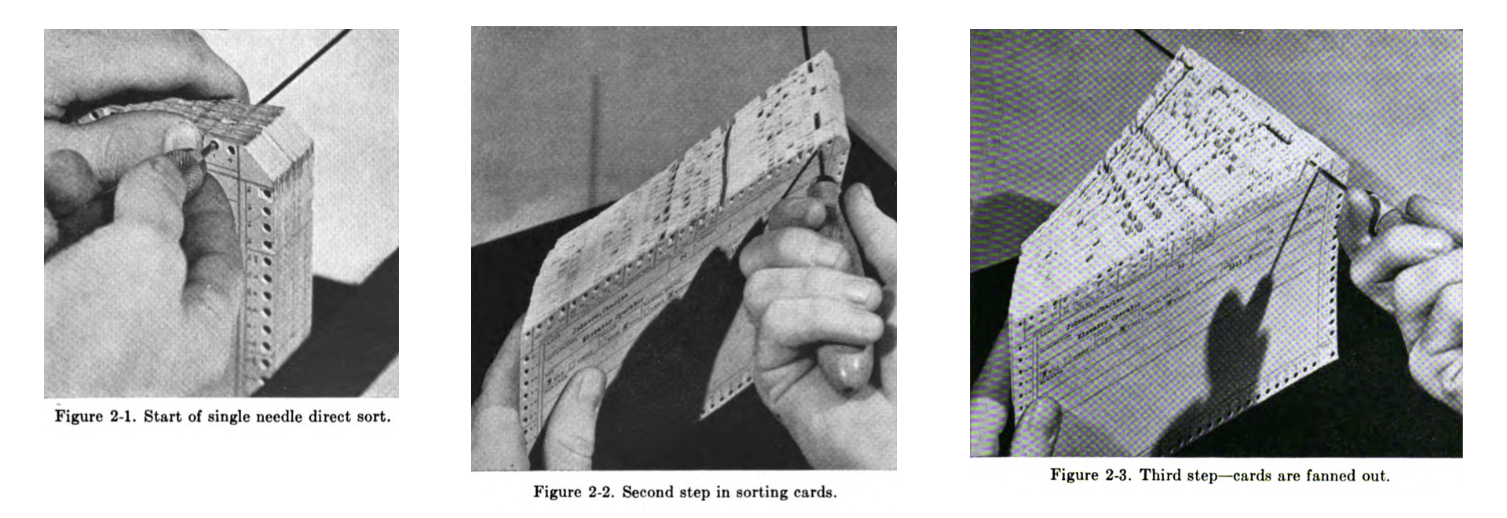
\includegraphics[scale =0.3]{images/Schede.png}
    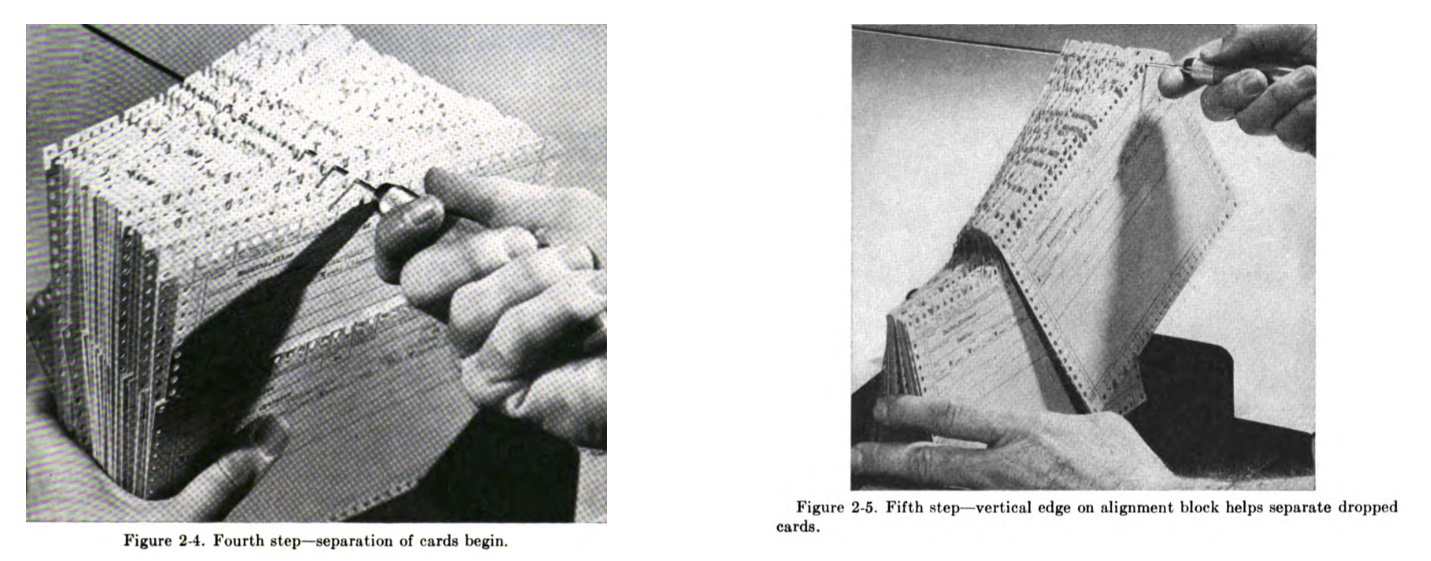
\includegraphics[scale =0.3]{images/Schede2.png}
    \caption{Gestione delle schede perforate.}
\end{figure}

\nt{Queste schede sono alla base di HyperCard, il primo sistema di ipertesto.}

\clm{}{}{
    La novità dell'utilizzo di queste "card" è l'utilizzo di unità minime di
    informazione, di insiemi di argomento ristretto che forniscono grande flessibilità  
    e capacità di manipolazione. Esse mettono a disposizione uno \fancyglitter{spazio di lavoro}
    che si può sfogliare\footnote{"Browse".}, a cui si possono fare aggiunte o correzioni e che
    permettono la costruzione di nuovi insiemi di nuclei di pensieri.
}

\paragraph{Utilità del computer:}

\begin{itemize}
    \item [$\Rightarrow$] Un computer è direttamente in grado di eseguire processi primitivi di manipolazione simbolica;
    \item [$\Rightarrow$] Con quei processi primitivi si possono costruire ogni altro processo che possa essere descritto da un linguaggio;
    \item [$\Rightarrow$] Un programma è una struttura di processi primitivi memorizzato sotto forma di simboli;
    \item [$\Rightarrow$] I computer hanno vari modi per memorizzzare simboli in modo che possano essere manipolati;
    \item [$\Rightarrow$] È possibile descrivere al computer nuovi simboli;
    \item [$\Rightarrow$] L'interfaccia è il punto di contatto tra l'uomo e la macchina (nascita dell'interazione uomo-macchina\footnote{Importante il time-sharing.});
    \item [$\Rightarrow$] 1962: \textit{un programma sperimentale di ricerca che è ancora lontano alcuni anni dalla fase presente della sua realizzazione} (DEMO del 1968).
\end{itemize}

\subsection{Panoramica della DEMO}

\paragraph{Sezioni:}

\begin{enumerate}
    \item La più celebre introduzione dell'informatica, descrive, in tono epico,
    la situazione che il sistema nLS intende aumentare con l'uso del computer;
    \item Manipolazione di testi, ri-organizzazione e visualizzazione sullo schermo del 
    computer. Livelli e outline. Hyperlinks;
    \item La metodologia di ricerca: l'approccio bootstrap (gruppo di ricerca) sul sistema nLS
    e sui principi di progettazione per lo sviluppo di sistemi di aumentazione;
    \item Periferiche: il mouse e il "keyset" (tastiera);
    \item Descrizione dell'hardware del sistema;
    \item Software di sistema (con Jeff Rulifson);
    \item Applicazioni del sistema: studio e modifica di articoli;
    \item Collaborazione online tra due persone attraverso condivisione di file e dello schermo (con Bill Paxton);
    \item Collegamento di computer in rete con condivisione di programmi ed esecuzione remota (viene annunciato ARPANET);
    \item Presentazione del gruppo di ricerca.
\end{enumerate}

\clm{}{}{
    Engelbart, inoltre, fu un sostenitore del lavoro di gruppo, infatti e nel suo gruppo di ricerca 
    che nasce la figura del \fancyglitter{facilitatore visuale}: una persona che durante le riunioni
    si occupa di disegnare su un foglio ciò che viene detto.

    Tuttavia, il laboratorio di Engelbart fallì perché propose un'immagine dell'utente che non ebbe successo (l'idea di un utente di personal computer che rimane circoscritto dal sistema).
    Molti dei collaboratori di Engelbart andarono a lavorare alla Xerox PARC che proponeva un'idea di utente diversa, più realistica.
}


%%%%%%%%%%%%%%%%%%%%%%%%%%%%%%%%%
% Licklider e Otlet
%%%%%%%%%%%%%%%%%%%%%%%%%%%%%%%%%

\definecolor{chaptergrey}{rgb}{1,0.75,0.8}

\ifnum\layout=2 
    \fancyhf{}      
    \renewcommand{\headrulewidth}{0pt}
    \renewcommand{\chaptermark}[1]{\markboth{#1}{}}

    \fancyhead[LE]{\nouppercase{\textbf{\textcolor{chaptergrey}{\chaptername}}~ \thechapter~ |~ \leftmark}}
    \fancyhead[RO]{\nouppercase{ \rightmark}}
    \fancyfoot[LE,RO]{\thepage}
    \fancypagestyle{plain}{         
    \fancyhf{}
    \fancyfoot[LE,RO]{\thepage}}    
 \else          
    \renewcommand{\headrulewidth}{0pt}
    \fancyhf{}                  
    \fancyhead[C]{\nouppercase{ \leftmark}}
    \fancyfoot[C]{\thepage}
\fi

\chapter{Licklider e Otlet}

\section{Licklider e le biblioteche del futuro}

Licklider (1915-1990) è stato uno psicoacustico che, nel 1950, iniziò ad appassionarsi
ai computer (al MIT). Partecipò sia alle "cene del Martedì" di Wiener\footnote{In cui si radunavano appassionati di cibernetica.} che 
alle Macy Conferences. Nel 1960 pubblicò un articolo intitolato \fancyglitter{Man-Computer Symbiosis} in cui
parla di una simbiosi uomo-computer in cui il computer è un collaboratore a cui si possono delegare
compiti di calcolo e di memorizzazione. 

\begin{figure}[h]
    \centering
    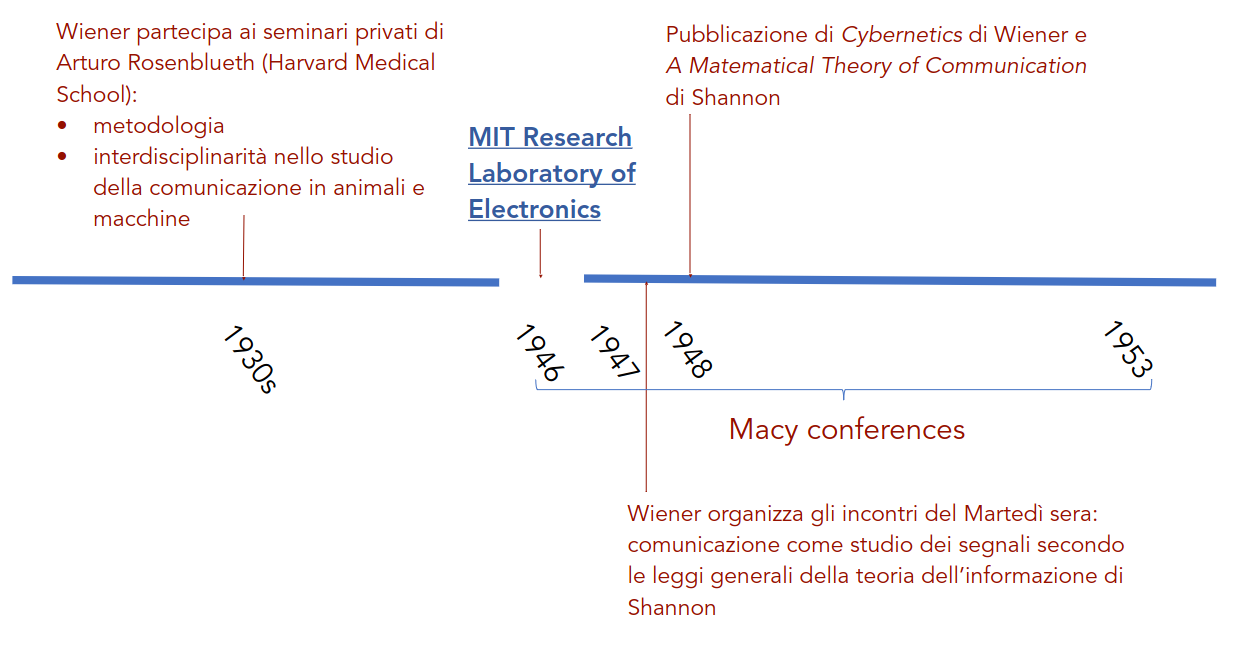
\includegraphics[scale=0.25]{images/MIT.png}
    \caption{Il MIT}
\end{figure}

\begin{itemize}
    \item [$\Rightarrow$] Licklider compie ricerche psico-acustiche (1943-1950);
    \item [$\Rightarrow$] Nel 1950 si appassiona ai computer;
    \item [$\Rightarrow$] Partecipa alle "cene del Martedì" di Wiener e alle Macy Conferences;
    \item [$\Rightarrow$] Lavora sul sistema SAGE (Semi-Automatic Ground Environment);
    \item [$\Rightarrow$] Vicepresidente della BBN (Bolt, Beranek and Newman), nel 1957 (inizia a lavorare sulle biblioteche del futuro);
    \item [$\Rightarrow$] Nel 1962 diventa direttore dell'ARPA (Advanced Research Projects Agency);
    \item [$\Rightarrow$] Convince Robert Fano a dirigere il progetto MAC (Multiple Access Computer)\footnote{Come visto nella prima parte del corso, nasce il \fancyglitter{time-sharing}.}.
\end{itemize}

\clm{}{}{C'è una leggenda secondo cui Licklider avrebbe persuaso Fano durante un viaggio in treno. Fano era un po'
scettico, ma conosceva Minsky, il ché era una garanzia di essere portati per l'informatica.
Inoltre aveva scritto un po' di programmi che funzionavano.}

\subsection{Man-Computer Symbiosis}

\paragraph{Prerequisiti per la simbiosi:}

\begin{itemize}
    \item [$\Rightarrow$] \fancyglitter{Time-sharing};
    \item [$\Rightarrow$] \fancyglitter{Estensione} della capacità e della velocità di accesso alla memoria;
    \item [$\Rightarrow$] \fancyglitter{Organizzazione} della memoria: accesso per nome o per schema con procedure di
    ricerca più veloci di quelle sequenziali (memorie associative, \fancyglitter{trie memory} di Fredkin);
    \item [$\Rightarrow$] \fancyglitter{Linguaggio}: gli ordini al computer specificano \fancyglitter{procedure}, all'uomo specificano \fancyglitter{obiettivi}.
\end{itemize}

\paragraph{Input e Output:}

\begin{itemize}
    \item [$\Rightarrow$] \fancyglitter{Riconoscimento} dei caratteri, \fancyglitter{immissione} dei dati in forma grafica;
    \item [$\Rightarrow$] \fancyglitter{Schermo gigante da parete} per la collaborazione e il coordinamento di gruppi\footnote{
        Vedrà la sua realizzazione negli anni '80 con il Computer-Supported Cooperative Work (CSCW), ma anche allo Xerox.
    };
    \item [$\Rightarrow$] \fancyglitter{Riconoscimento} del parlato.
\end{itemize}

\dfn{La rete intergalattica (1963)}{
    Nel 1963 Licklider scrive un articolo come Memorandum per i "Member and Affiliates of the Intergalactic Computer Network" 
    in cui invita le università a collegare i loro computer in una rete 
    per condividere risorse software.
}

\clm{}{}{Sulla West Coast, il movimento hippie\footnote{Nato nella zona di San Francisco.},
    concepisce l'idea di dare all'individuo la completa libertà che può essere messa
    in parallelo con l'idea di personal computer (nn c'è condivisione di risorse, il computer è individuale).

}

\subsection{Le critiche al libro}

Nel libro \fancyglitter{Libraries of the Future} (1965) Licklider esplora
lo studio di classi di informazioni e domini di conoscenza, ci si concentra sui
concetti, sui principi e sulle idee dei libri più che sul loro aspetto tangibile.
Licklider vuole modificare gli \fancyglitter{schemi} impiegati per pensare alle biblioteche.

\begin{center}
    \fancyglitter{Componenti} $\rightarrow$ \fancyglitter{Pagine}

    \fancyglitter{Sottosistemi} $\rightarrow$ \fancyglitter{Volumi}

    \fancyglitter{Sistemi} $\rightarrow$ \fancyglitter{Biblioteche}
\end{center}

\begin{figure}[h]
    \centering
    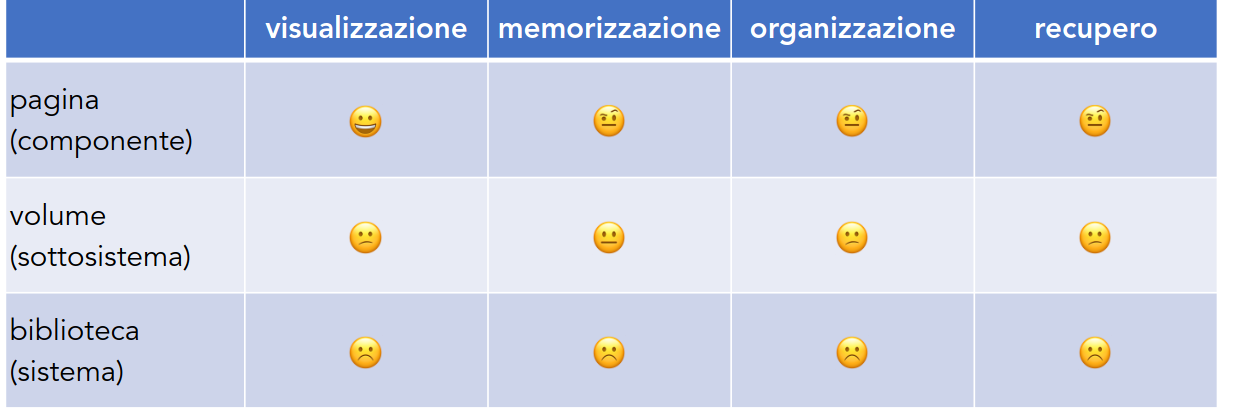
\includegraphics[scale=0.35]{images/Schemi.png}
    \caption{Schemi tradizionali.}
\end{figure}

\paragraph{Nelle prime pagine di Libraries of the Future vengono mosse delle critiche alla struttura e al concetto di libro:}

\begin{itemize}
    \item [$\Rightarrow$] La pagina può essere facilmente visualizzata e modificata, ma più pagine (libri) sono pesanti;
    \item [$\Rightarrow$] I libri contengono troppe informazioni e ciò nasconde le parti utili;
    \item [$\Rightarrow$] I libri sono scarsi anche dal punto della visualizzazione e del recupero delle informazioni\footnote{I problemi di indicizzazione già messi in evidenza da Bush.};
    \item [$\Rightarrow$] I testi sono passivi;
    \item [$\Rightarrow$] Dato che i libri (collezioni di pagine) diminuiscono i vantaggi della pagina, le biblioteche (collezioni di libri) diminuiscono i vantaggi dei libri.
\end{itemize}

\paragraph{Problema (passività della pagina stampata):}
\begin{itemize}
    \item [$\Rightarrow$] Il trasferimento di informazioni contenuta dai libri richiede lo spostamento del lettore, del libro o di entrambi;
    \item [$\Rightarrow$] Le operazioni di elaborazione del contenuto devono essere eseguite dal lettore.
    
\end{itemize}

\paragraph{Proposta di soluzione:} unire biblioteche e computer in un \fancyglitter{sistema procognitivo} (o biblioteca del futuro) per facilitare
l'interazione umana con informazione manipolabile e trasformabile.

\begin{figure}[h]
    \centering
    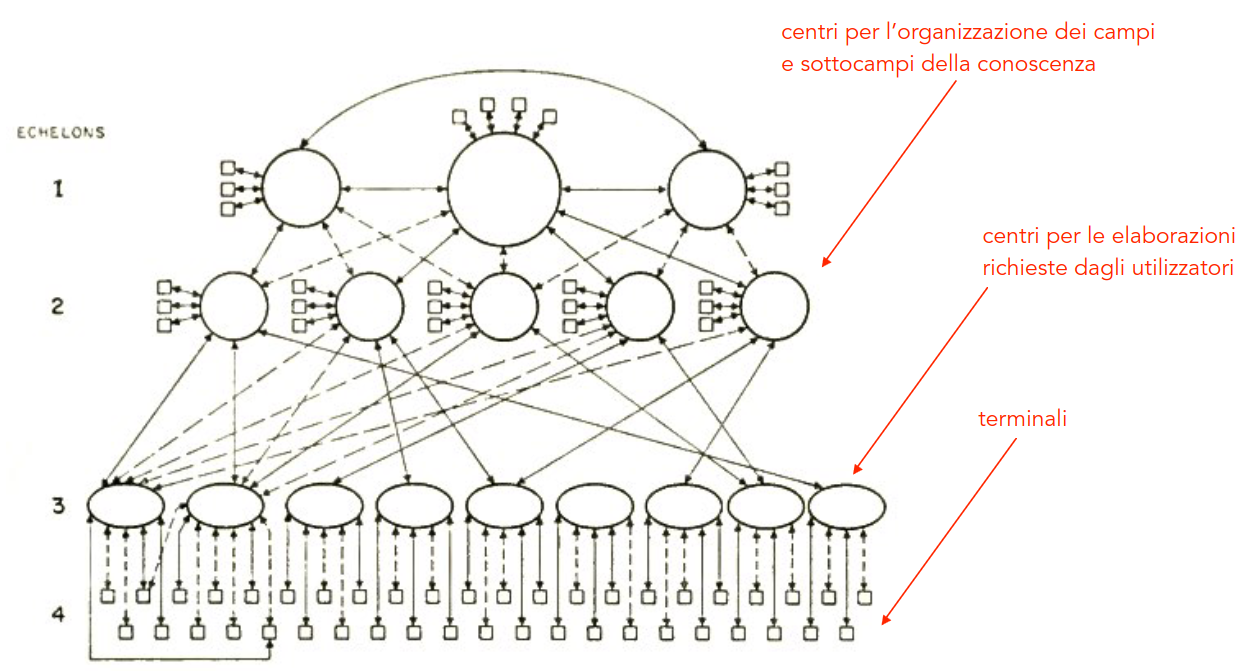
\includegraphics[scale=0.28]{images/SistemiP.png}
    \caption{Una biblioteca del futuro.}
\end{figure}

\paragraph{Riassunto dei difetti (\textcolor{red}{\XSolidBrush}) e dei pregi (\textcolor{green}{\Checkmark}) degli schemi tradizionali:}

\begin{itemize}
    \item [\textcolor{red}{\XSolidBrush}] Schema della biblioteca fisica con scaffali, schede, banchi di consegna, sale di lettura;
    \item [\textcolor{red}{\XSolidBrush}] Schema del libro fisico come archivio passivo di informazione stampata;
    \item [\textcolor{red}{\XSolidBrush}] Schema della pagina stampata come strumento per la memorizzazione a lungo termine;
    \item [\textcolor{green}{\Checkmark}] Gerarchie di segmenti di testo (carattere, parola, frase, paragrafo, capitolo, libro);
    \item [\textcolor{green}{\Checkmark}] La suddivisione in informazione testuale, grafica e figurativa;
    \item [\textcolor{green}{\Checkmark}] Le parti dei documenti (indice, prefazione, appendice, bibliografia, ecc.);
    \item [\textcolor{green}{\Checkmark}] Tipologie di pubblicazioni (libri, riviste, giornali, ecc.);
    \item [\textcolor{green}{\Checkmark}] Infrastrutture come catalogo, indice, etc..
\end{itemize}

\nt{Inoltre i "centri di calcolo" sono inefficaci nel tempo. Ed è proprio da
questo che si reinventa il calcolo in chiave contemporanea (time-sharing).}

\section{Otlet e la documentazione universale}

Paul Otlet (1868-1944) è stato un avvocato belga. Nel 1895 fonda l'Institut International de Bibliographie (IIB) a cui
si poteva scrivere per avere risposte in merito a domande bibliografiche. Nel 1904 Otlet e Henri La Fontaine, 
un avvocato e politico belga, crearono la \fancyglitter{Classificazione Decimale Universale} (una variante della Dewey). Nel 1919 Otlet creò il \fancyglitter{Palais Mondial}
e nel 1924 il \fancyglitter{Mundaneum}.

\subsection{Il futuro del libro}

Otlet affrontò il problema della \fancyglitter{crescita disordinata della letteratura}
nelle scienze sociali (1892 - Sulla bibliografia).
Per Otlet bisognava ridurre tutti i \fancyglitter{fatti osservati}, rimuovendo
tutte le \fancyglitter{interpretazioni possibili} trasformandoli in leggi, \fancyglitter{statistiche} e \fancyglitter{fonti}\footnote{Idea figlia del Positivismo.}.
Subito dopo gli elementi ottenuti verrebbero trasferiti su schede classificate con la 
Classificazione Decimale Universale. Così si arriverebbe alla creazione di un \fancyglitter{cervello artificiale}.
Nel 1918 Otlet pubblica "Trasformazioni nell'apparato bibliografico delle scienze" in cui viene messo in risalto il problema
della crescente produzione di libri\footnote{Ripreso da Bush.} e si parla di un miglioramento delle biblioteche\footnote{Ripreso da Licklider.}. In
questo testo vengono introdotte alcune idee:

\begin{itemize}
    \item [$\Rightarrow$] \fancyglitter{Repertorio};
    \item [$\Rightarrow$] \fancyglitter{Classificazione};
    \item [$\Rightarrow$] \fancyglitter{Ufficio della documentazione}.
\end{itemize}

\paragraph{Otlet criticò il libro:}

\begin{itemize}
    \item [$\Rightarrow$] Non è pratico per la consultazione di specifici passaggi;
    \item [$\Rightarrow$] È un'entità completa a cui non si può aggiungere nulla;
    \item [$\Rightarrow$] Rende difficile il collegamento di elementi correlati (richiede indicizzazione).
\end{itemize}

\nt{Probabilmente Licklider non conosceva Otlet, ma le conclusioni a cui sono giunti sono molto simili.}

\dfn{Repertorio}{
Il repertorio separa ciò che nel libro è unito e lo riduce a elementi
a cui viene dedicata una scheda. Non esiste la \newfancyglitter{rilegatura}, ma
le schede vengono tenute insieme in modo da poter essere riordinate, eliminate
o intercalate da nuove schede\footnote{Ricorda un quaderno ad anelli. Inoltre ci si può vedere un rimando all'idea di schede di Engelbart.}.
Il repertorio permette di \newfancyglitter{suddividere} un libro secondo il suo
contenuto: un libro è solo un'unica riga continua suddivisa per conformarsi alle pagine\footnote{Un po' come se fosse scritto sul nastro di una macchina di Turing.}.
}

\clm{}{}{
    Il prof. Cardone esprime disappunto riguardo il significato di "pagina" di Otlet.
    La pagina ha una sua portata e persino i margini possono essere usati per esprimere qualcosa.
}

\dfn{Classificazione UDC}{
    La Classificazione Decimale Universale (UDC) è un sistema di classificazione bibliografica
    che si basa su un sistema di numeri decimali. È simile al linguggio ideale per 
    l'organizzazione della conoscenza. È decimale perché divisa in 10 classi, suddivise in almeno 10
    gruppi e ogni gruppo in almeno 10 divisioni.
}

\nt{La notazione UDC permette di creare senza limitazioni codici di classi.}

\dfn{Ufficio della documentazione}{
Le biblioteche sono \newfancyglitter{musei di libri}. Le loro collezioni sono 
relative alle esigenze di documentazione. Per rimediare a ciò, Otlet propose
l'idea di un \newfancyglitter{ufficio della documentazione} che avrebbe come punto
di partenza queste collezioni e dovrebbe stabilire dei collegamenti tra loro in modo da 
formare il \newfancyglitter{Libro Universale}\footnote{Questo ricorda ciò che saranno gli ipertesti di Nelson.}.
}

\subsection{Il Traité de documentation}

Nel 1934 Otlet pubblicò il \fancyglitter{Traité de documentation} in cui vengono sistematizzate
le proprie idee, parzialmente realizzate dal Mundaneum. Otlet studiò la possibilità di
\fancyglitter{macchine a supporto dei processi intellettuali}:

\begin{itemize}
    \item [$\Rightarrow$] Una \fancyglitter{scrivania} con superfici separate per la gestione di 
    progetti paralleli;
    \item [$\Rightarrow$] Macchine per la consultazione remota di documenti;
    \item [$\Rightarrow$] Una scrivania \fancyglitter{senza libri} ma con solo \fancyglitter{schermo e telefono}.
\end{itemize}

\nt{La standardizzazione della creazione, organizzazione, pubblicazione ed elaborazione
dei documenti favoriranno la creazione di una \fancyglitter{Rete Universale di Documentazione}.}

\clm{}{}{
    Nel 1968, Licklider collabora con Taylor (direttore di una sezione dello Xerox PARC) per un articolo,
    "The Computer as a Communication Device"\footnote{Scritto per via della sua esperienza nel laboratorio 
    di Engelbart.}, in cui si parla di una rete di computer che permetta la condivisione di risorse.
    Ossia il fatto che, nel giro di pochi anni, gli utenti comunicheranno più efficacemente
    attraverso una macchina che faccia a faccia. 

}


%%%%%%%%%%%%%%%%%%%%%%%%%%%%%%%%%
% Nelson e Kay
%%%%%%%%%%%%%%%%%%%%%%%%%%%%%%%%%

\definecolor{chaptergrey}{rgb}{0,0.13, 0.38}

\ifnum\layout=2 
    \fancyhf{}      
    \renewcommand{\headrulewidth}{0pt}
    \renewcommand{\chaptermark}[1]{\markboth{#1}{}}

    \fancyhead[LE]{\nouppercase{\textbf{\textcolor{chaptergrey}{\chaptername}}~ \thechapter~ |~ \leftmark}}
    \fancyhead[RO]{\nouppercase{ \rightmark}}
    \fancyfoot[LE,RO]{\thepage}
    \fancypagestyle{plain}{         
    \fancyhf{}
    \fancyfoot[LE,RO]{\thepage}}    
 \else          
    \renewcommand{\headrulewidth}{0pt}
    \fancyhf{}                  
    \fancyhead[C]{\nouppercase{ \leftmark}}
    \fancyfoot[C]{\thepage}
\fi

\chapter{Nelson e Kay}

\section{Verso gli ipertesti: Ted Nelson}

Ted Nelson nacque nel 1937, i suoi genitori (un'attrice e un regista) divorziarono nel 1939 e lui venne cresciuto dai nonni
materni. Nelson studiò filosofia e si laureò in sociologia (1963) prendendo un dottorato nel 
2002 (in realtà la sua tesi è una riproposizione di idee avute nel 1959).
Le sue pubblicazioni più importanti sono:

\begin{itemize}
    \item [$\Rightarrow$] \fancyglitter{Complex Information Processing: A File Structure for the Complex, the Changing and the Indeterminate} (1965): 
    articolo tecnico in cui si introduce il concetto di \fancyglitter{ipertesto} con le strutture dati collegate;
    \item [$\Rightarrow$] \fancyglitter{Computer Lib/Dream Machines} (1974): libro autopubblicato.
    Il titolo è doppio perché il libro è doppio, ossia si legge in due direzioni.
    Inoltre la grafica richiama una pubblicazione della controcultura hippie (curata da Stewart Brand),
    ossia il \fancyglitter{Whole Earth Catalog}\footnote{Catalogo di oggetti (in particolar modo libri)
    messi in vendita. Molti testi appartenevano alla libreria dello Xerox PARC.};
    \item [$\Rightarrow$] \fancyglitter{Literary Machines} (1981): descrizione del sistema Xanadu.
\end{itemize}

\clm{}{}{
    Nelson fa il compleanno lo stesso giorno del prof. Cardone.
}

\clm{}{}{

\paragraph{Nelson ha anche girato un video "estremo":}

\begin{itemize}
    \item [$\Rightarrow$] \fancyglitter{Silicon Valley Story} (1992): non si capisce niente, surreale. Ma compaiono personaggi come 
    Timoty Leary (profeta delle droghe psichedeliche\footnote{AKA psicologo di Harvard.}), Douglas Engelbart e Stuart Brand.
\end{itemize}
}

\subsection{Xanadu e Parallel Textface}

Anche Nelson fa parte del gruppo di persone che ha letto \fancyglitter{As We May Think} di Vannevar Bush.
Nelson scrive un articolo, \fancyglitter{As We Will Think}, dove analizza il testo di Bush. 

\paragraph{Per Nelson il memex può essere considerato come:}

\begin{itemize}
    \item [$\Rightarrow$] Una console personale per la \fancyglitter{presentazione}, la 
    \fancyglitter{manipolazione} (editing) e l'\fancyglitter{archiviazione} (file);
    \item [$\Rightarrow$] Una \fancyglitter{rete di alimentazione per la distribuzione di documenti} in formato digitale\footnote{Bush pensava alla condivisione su microfilm.};
    \item [$\Rightarrow$] Un \fancyglitter{nuovo tipo di documento} (ipertesto), pensato per essere ricevuto e spedito.
\end{itemize}

\subsubsection{}

In As We Will Think Nelson parla delle interpretazioni sbagliate che sono 
state date all'articolo di Bush. Per esempio un interesse di Bush nel rendere 
più efficiente l'indicizzazione (Information retrieval) che in realtà non c'era.
Come abbiamo visto il memex è in contrasto con tutto ciò.
Nel \fancyglitter{sistema Xanadu} Nelson spiega la sua interpretazione del 
memex e delle idee di Bush.

\dfn{Xanadu}{
    Xanadu è un sistema stand-alone, costruito su un minicomputer con vari 
    metodi di recupero delle informazioni automatici e manipolazione del database del 
    sistema soggiacente tramite \newfancyglitter{theaters} (front-end).
}

\cor{Parallel Textface}{
    Il più importante dei theaters è il \fancyglitter{Parallel Textface}: un 
    sistema testuale di una certa potenza e raffinatezza.

    L'utente siede davanti allo schermo con una tastiera o una lightpen 
    e può scrivere, cancellare, spostare, copiare e incollare testo. La 
    memorizzazione è digitale.
}

\nt{Il Parallel Textface è un'implementazione delle "note e commenti marginali" di Bush.}

\subsection{Ipertesti}

Nel 1967, Nelson scrisse delle note\footnote{Mai pubblicate.} significative sugli ipertesti.

\clm{}{}{Le sue note si possono trovare nell'archivio di Nelson. Purtroppo
Nelson è molto disordinato quindi molte delle sue note sono incomprensibili fuori dal contesto,
scarabocchi su carta, etc.}

\begin{figure}[h]
    \centering
    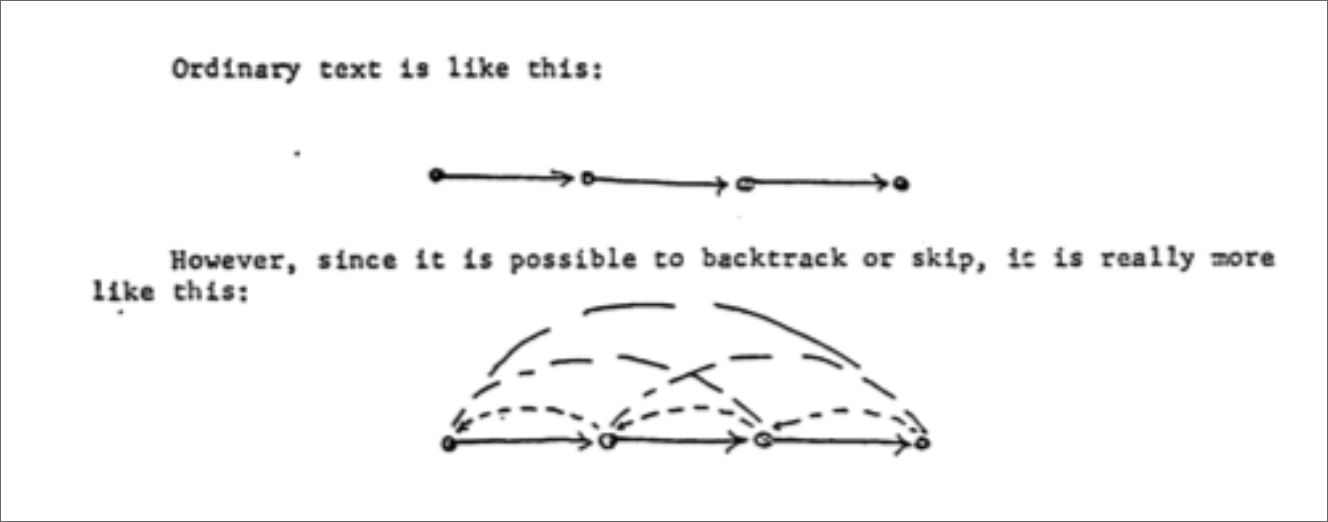
\includegraphics[scale=0.35]{images/H1.png}
\end{figure}

\begin{figure}[h]
    \centering
    
\includegraphics[scale=0.25]{images/H2.png}
    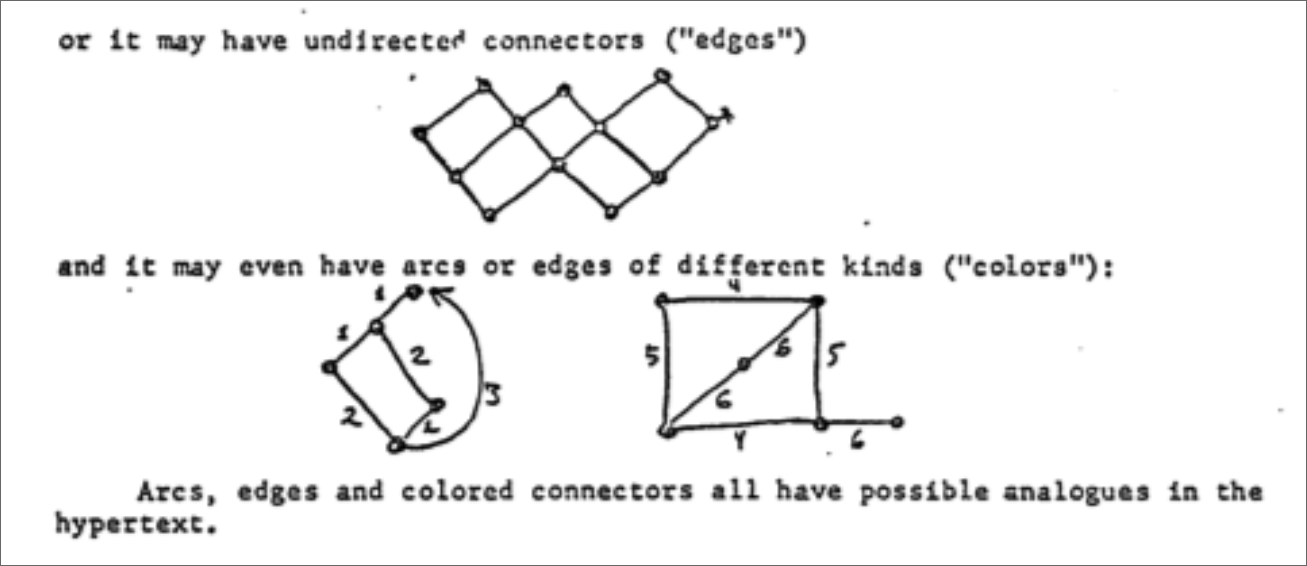
\includegraphics[scale=0.25]{images/H3.png}
\end{figure}

\nt{Un esempio di ipertesto come inteso da Nelson sono 
le mappe mentali o le mappe concettuali.
}

\clm{}{}{
    Engelbart, al contrario di Nelson, era più un fan dei testi strutturati
    ad albero diviso in capitoli, sezioni, sottosezioni,
    etc. dove sono le etichette a stabilire dei link tra parti 
    diverse di un testo (Un po' come i miei appunti).
}

\dfn{Connettori}{
    Si hanno due tipi di \newfancyglitter{annotazioni} (connettori):
    \begin{itemize}
        \item [$\Rightarrow$] \fancyglitter{Tag}: marcatore nel testo a cui
        è allegata una breve nota o spiegazione;
        \item [$\Rightarrow$] \fancyglitter{Link}: collegamento tra due elementi testuali. 
        È un salto da un punto a un altro. 
    \end{itemize}
}

\dfn{Piste}{
    La \fancyglitter{pista} (trail) è una sequenza di documenti, estratti
    di documenti e commenti su essi. Si stabilisce realizzando degli accoppiamenti.
}

\cor{Tipi di piste}{
    \begin{itemize}
        \item [$\Rightarrow$] \fancyglitter{Side trail}: pista laterale,
        si dirama da una pista principale;
        \item [$\Rightarrow$] \fancyglitter{Skip trail}: sottoinsieme 
        di una pista principale, contiene solo i punti salienti.
    \end{itemize}
}

\clm{}{}{
    Tutto ciò che si fa in questo corso è opinabile e soggetto a eventuali critiche.
    È necessario riflettere su queste cose, per esempio: in un ipertesto, che 
    nasce per contrastare la struttura sequenziale, bisogna comunque tracciare delle 
    piste, ricadendo nell'inevitibilità della sequenzialità.

    La critica di Nelson al testo sequenzializzato è a sua volta criticabile.
}

\qs{}{Ma quindi che cos'è, per Nelson, un ipertesto?}

\dfn{Ipertesto}{
    Un ipertesto è una struttura del testo che non può essere comodamente
    stampata.
}

\cor{Stretchtext}{
    Un esempio di ipertesto è lo \fancyglitter{stretchtext}, un testo che 
    può essere allungato a piacimento.
}

\nt{Interi ipertesti possono essere collegati tra loro formando dei libri.
Idee già viste nella classificazione di Otlet, nelle biblioteche del futuro di Licklider e 
nel memex di Bush.}

\dfn{Transclusion}{
    La \newfancyglitter{transclusion} è un'operazione che permette di condividere fisicamente
    un testo in altri testi.
}

\cor{Collateration}{
    La \fancyglitter{collateration} è un'operazione che permette di creare collegamenti
    con \fancyglitter{zippered lists} (liste con cerniere) per mezzo di link visualizzabili.
}

\begin{figure}[h]
    \centering
    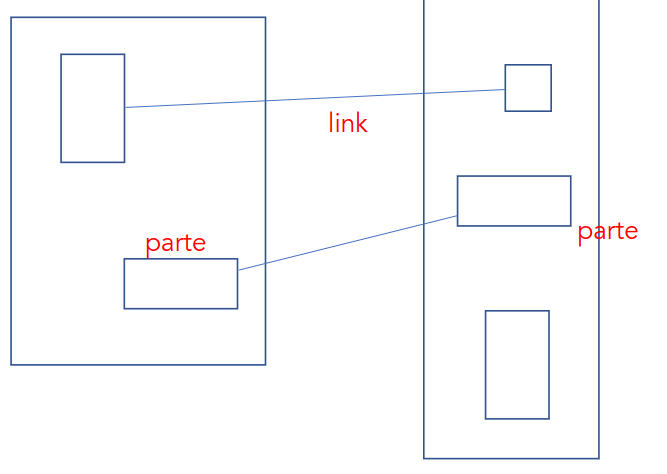
\includegraphics[scale=0.45]{images/Col.png}
\end{figure}

\nt{Esempi di collateration sono le note a margine, le note a piè di pagina, sommari, indici, intestazioni, etc.

Ossia il paratesto.}

\dfn{Docuverso}{
    Il \newfancyglitter{docuverso} è un nuovo sistema di iperpubblicazione che
    contiene un insieme di documenti collegati tra loro, grazie alla transclusion.

    Questo è alla base di Xanadu.
}

\subsection{Implemetazione degli ipertesti}


\begin{itemize}
    \item [$\Rightarrow$] \fancyglitter{Pianificazione di strutture non lineari}: per esempio delle mostre;
    \item [$\Rightarrow$] \fancyglitter{Strutture informative in forma grafica}: per esempio diagrammi PERT e programmi;
    \item [$\Rightarrow$] \fancyglitter{Hypermedia}: per esempio alcuni film, fumetti, etc.
\end{itemize}

\dfn{NoteCards}{
    Le \newfancyglitter{NoteCards} sono un sistema di Hypermedia per 
    rappresentare e manipolare informazioni. Sono state sviluppate a 
    Xerox PARC.
}

\ex{NoteCards}{
    \begin{center}
        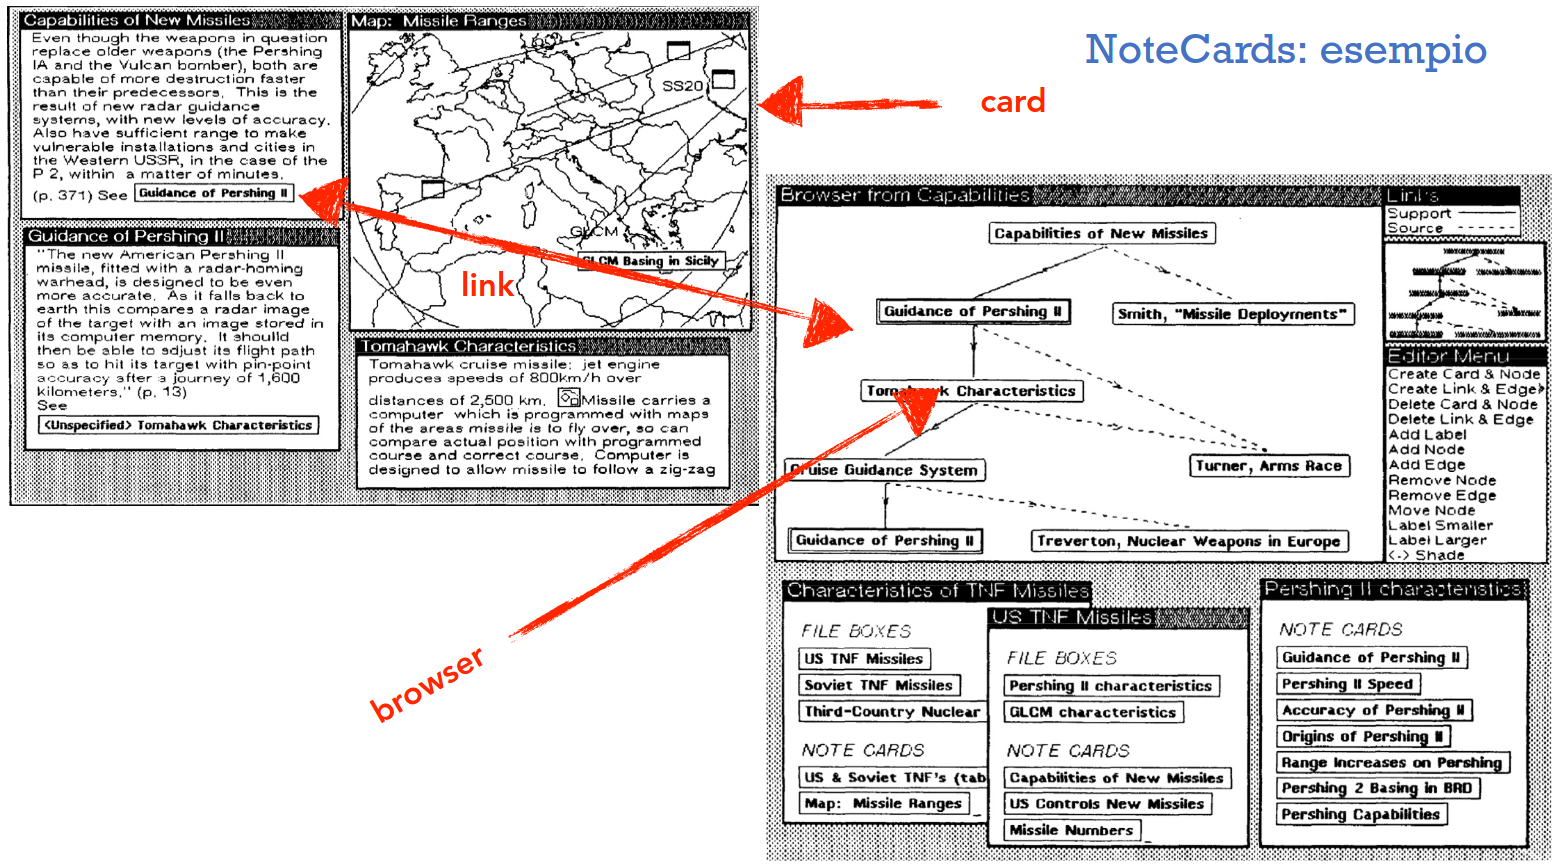
\includegraphics[scale=0.25]{images/NC.png}
    \end{center}
}

\nt{Successivamente si può parlare di HyperCard, che veniva regalato con i Macintosh.
HyperCard è un sistema di pile di schede e aveva una funzione didattica.}

\dfn{Thinkertoys}{
    I \newfancyglitter{Thinkertoys} sono un sistema di visualizzazione
    per computer che aiuta a considerare alternativa complesse.
}
\paragraph{Alternative complesse:}
\begin{itemize}
    \item [$\Rightarrow$] Progetti alternativi;
    \item [$\Rightarrow$] Discrepanze tra le testimonianze;
    \item [$\Rightarrow$] Bozze successive di un documento.
\end{itemize}

\dfn{Fantics}{
    La \newfancyglitter{fantics} (o fantica) è:
    \begin{itemize}
        \item [$\Rightarrow$] L'arte e la scienza della presentazione;
        \item [$\Rightarrow$] Tecniche di presentazione: scrittura, regia, realizzazione di filmati, etc.
        \item [$\Rightarrow$] I media, la loro analisi, la loro progettazione, etc.;
        \item [$\Rightarrow$] La progettazione di sistemi per le presentazioni.
    \end{itemize}
    
}

\nt{Nelson parla di spazio fantico: uno spazio creato ad arte per la 
presentazione di informazioni. Da ricordare la figura del 
"Facilitatore visuale" nata nel laboratorio di Engelbart.}

\section{Il Computer come Medium: Alan Kay}

Alan Kay è nato nel 1940. Dal punto di vista della storia dell'informatica è importante perché creò lo Smalltalk\footnote{Visto nella prima parte del corso.}
Nel 1962 si arruola nell'esercito e analizza il sistema per condividere i dati tra basi militari:

\begin{itemize}
    \item [$\Rightarrow$] La prima parte era una \fancyglitter{sequenza di puntatori} alla seconda parte;
    \item [$\Rightarrow$] La seconda parte conteneva le \fancyglitter{procedure} utilizzate per accedere e modificare i dati della terza parte;
    \item [$\Rightarrow$] La terza parte conteneva i \fancyglitter{record} con i dati.
\end{itemize}

\begin{figure}[h]
    \centering
    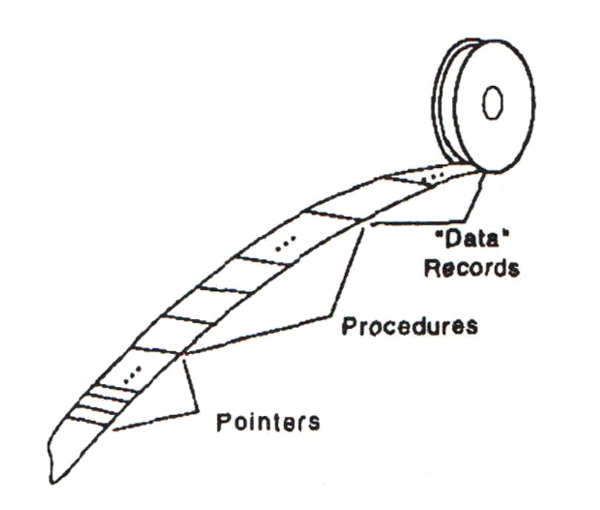
\includegraphics[scale=0.5]{images/Data.png}
\end{figure}
\pagebreak
\subsection{Gli inizi}

Dopo la laurea Kay entra nel programma di dottorato\footnote{Era stato creato da poco grazie a Licklider.} all'università di Utah.
Qua scopre \fancyglitter{Sketchpad} (programma di grafica interattiva) di Ivan Sutherland.

\dfn{Simula 67}{
    Il \newfancyglitter{Simula 67} è un linguaggio di programmazione orientato agli oggetti
    inventato da Ole-Johan Dahl e Kristen Nygaard.
}

\paragraph{Kay osservò le relazioni tra Sketchpad e Simula 67 (con una metafora biologica):}

\begin{itemize}
    \item [$\Rightarrow$] Le cellule ("instances") si conformano ai comportamenti "master";
    \item [$\Rightarrow$] Le cellule sono autonome e comunicano tra loro scambiandosi messaggi;
    \item [$\Rightarrow$] Le cellule diventano parti diverse di un organismo a seconda del contesto.
\end{itemize}

\nt{Questa metafora sarà alla base del Smalltalk.}

\paragraph{Altre influenze che hanno dato forma al lavoro di Kay:}

\begin{itemize}
    \item [$\Rightarrow$] \fancyglitter{McLuhan}: il medium è il messaggio;
    \item [$\Rightarrow$] \fancyglitter{Papert e il linguaggio LOGO}\footnote{Visti nel corso "Metodologie
    e Tecnologie Didattiche per l'Informatica".}: il computer come strumento per l'apprendimento.
\end{itemize}

\begin{figure}[h]
    \centering
    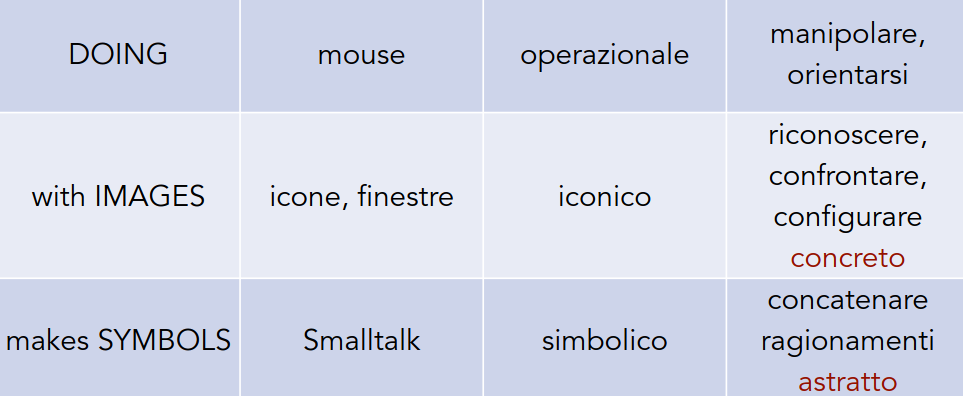
\includegraphics[scale=0.45]{images/App.png}
    \caption{Apprendimento secondo Kay.}
\end{figure}


\subsection{Il Dynabook}

\nt{Il computer è un medium di comunicazione:
\begin{itemize}
    \item [$\Rightarrow$] Conversazionale;
    \item [$\Rightarrow$] Attivo;
    \item [$\Rightarrow$] Universale: può essere usato per simulare qualsiasi altro media;
    \item [$\Rightarrow$] Dinamico.
\end{itemize}
}

\dfn{Dynabook}{
    Il \newfancyglitter{Dynabook} è un computer portatile per bambini, con un'interfaccia grafica e un linguaggio di programmazione semplice.
}

\nt{Non molto diverso da un tablet.}

\begin{figure}[h]
    \centering
    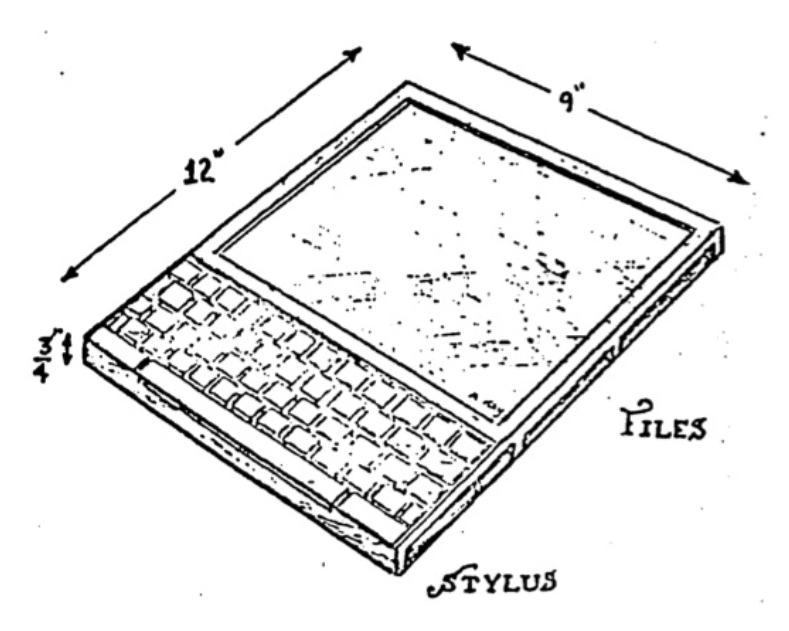
\includegraphics[scale=0.45]{images/Dyn.png}
    \caption{Il Dynabook.}
\end{figure}

\paragraph{Caratteristiche del Dynabook:}

\begin{itemize}
    \item [$\Rightarrow$] Possibilità di memorizzazione interattiva;
    \item [$\Rightarrow$] Lettura di testi ordinari e ipertesti;
    \item [$\Rightarrow$] Fonts personalizzabili;
    \item [$\Rightarrow$] WYSIWYG\footnote{
        What You See Is What You Get: il testo visualizzato sullo schermo è uguale a quello stampato.
    } nell'editing di testi;
    \item [$\Rightarrow$] Finestre multiple e sovrapponibili;
    \item [$\Rightarrow$] Sensorializzazione di processi dinamici;
    \item [$\Rightarrow$] Animazione e musica;
    \item [$\Rightarrow$] Programmazione;
    \item [$\Rightarrow$] Simulazione.
\end{itemize}

\dfn{Xerox ALTO}{
    L'Xerox ALTO\footnote{Visto nella prima parte del corso.} è un tentativo di realizzare il Dynabook.
}

\dfn{Xerox NoteTaker}{
    Il \newfancyglitter{Xerox NoteTaker} fu il primo computer portatile utilizzato in aereo da 
    Douglas Fairbairn (informatico che si occupò di linguaggi funzionali).
}

\subsection{Smalltalk}

\dfn{Smalltalk}{
    Lo \newfancyglitter{Smalltalk} è un linguaggio di programmazione orientato agli oggetti
    che avrebbe dovuto essere usato per programmare il Dynabook.
}

\paragraph{Principi dello Smalltalk:}

\begin{itemize}
    \item [$\Rightarrow$] \fancyglitter{Oggetti}: tutto è un oggetto;
    \item [$\Rightarrow$] \fancyglitter{Messaggi}: gli oggetti comunicano scambiandosi messaggi (oggetti);
    \item [$\Rightarrow$] Gli oggetti hanno \fancyglitter{memoria privata};
    \item [$\Rightarrow$] Ogni oggetto è istanza di una \fancyglitter{classe};
    \item [$\Rightarrow$] Le classi contengono i \fancyglitter{comportamenti} comuni alle loro istanze;
    \item [$\Rightarrow$] Per valutare un programma il controllo è passato al primo oggetto e il resto è 
    interpretato come un suo messaggio.
\end{itemize}

\begin{figure}[h]
    \centering
    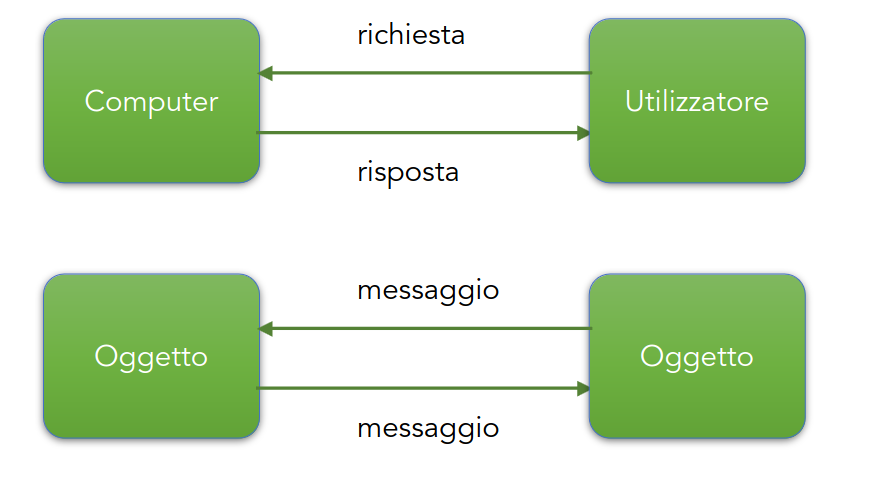
\includegraphics[scale=0.5]{images/Small.png}
    \caption{Smalltalk.}
\end{figure}


\section{Per concludere: una storia alternativa}

\subsection{Whole Earth Catalog e Computer Lib/Dream Machines}

Il \fancyglitter{Whole Earth Catalog} fu una pubblicazione curata da Stewart Brand.
Si trattava di un catalogo di oggetti (in particolar modo libri) messi in vendita, con 
al centro il motto "Access to tools", garantendo l'accesso a strumenti e conoscenze.
Si trattava di un'opera di controcultura hippie e di un Google ante litteram (come detto da Steve Jobs).

\paragraph{Un articolo è elencato nel WEC se:}

\begin{itemize}
    \item [$\Rightarrow$] È utile come strumento;
    \item [$\Rightarrow$] Serve per l'istruzione;
    \item [$\Rightarrow$] È di buona qualità o di basso costo;
    \item [$\Rightarrow$] È facilmente disponibile per corrispondenza.
\end{itemize}


\paragraph{Sezioni del WEC:}

\begin{itemize}
    \item [$\Rightarrow$] Understanding Whole Systems;
    \item [$\Rightarrow$] Shelter and Land Use;
    \item [$\Rightarrow$] Industry and Craft;
    \item [$\Rightarrow$] Communications;
    \item [$\Rightarrow$] Community;
    \item [$\Rightarrow$] Nomadics;
    \item [$\Rightarrow$] Learning.
\end{itemize}

\nt{Si può considerare il WEC come un'ipertesto in formato cartaceo.}

\dfn{Computer Lib/Dream Machines}{
    Il \newfancyglitter{Computer Lib/Dream Machines} è il già citato libro pubblicato da Ted Nelson.
    È ispirato al WEC e ha una grafica simile.   
}

\nt{Successivamente si sviluppo il \fancyglitter{Whole Universe Catalog} di Kirk Kelley (ex sviluppatore nel laboratorio di Engelbart),
che era un'opera di controcultura hippie, ma non fu mai finanaziato.}





%%%%%%%%%%%%%%%%%%%%%%%%%%%%%%%%%
% Letture
%%%%%%%%%%%%%%%%%%%%%%%%%%%%%%%%%

\definecolor{chaptergrey}{rgb}{0.21,0.37,0.23}

\ifnum\layout=2 
    \fancyhf{}      
    \renewcommand{\headrulewidth}{0pt}
    \renewcommand{\chaptermark}[1]{\markboth{#1}{}}

    \fancyhead[LE]{\nouppercase{\textbf{\textcolor{chaptergrey}{\chaptername}}~ \thechapter~ |~ \leftmark}}
    \fancyhead[RO]{\nouppercase{ \rightmark}}
    \fancyfoot[LE,RO]{\thepage}
    \fancypagestyle{plain}{         
    \fancyhf{}
    \fancyfoot[LE,RO]{\thepage}}    
 \else          
    \renewcommand{\headrulewidth}{0pt}
    \fancyhf{}                  
    \fancyhead[C]{\nouppercase{ \leftmark}}
    \fancyfoot[C]{\thepage}
\fi
\afterpage{\blankpage}

\chapter{Letture}

Questo capitolo contiene dei mini-riassunti delle Letture
obbligatorie per l'esame. Poiché è possibile e consigliato consultare
i documenti durante l'esame, questi riassunti hanno la funzione di 
aiutare a ricordare i concetti principali per facilitare la navigazione 
e la consultazione.

\begin{itemize}
    \item [$\Rightarrow$] Vannevar Bush, \href{https://informatica.i-learn.unito.it/pluginfile.php/368484/mod_resource/content/7/Bush%20%281945%29.pdf}{Come potremmo pensare}, 1945;
    \item [$\Rightarrow$] Susan Barnes, \href{https://informatica.i-learn.unito.it/pluginfile.php/368474/mod_resource/content/2/Barnes%2C%20S.B.%20--%20Douglas%20Carl%20Engelbart-%20developing%20the%20underlying%20concepts%20for%20contemporary%20computing.pdf}{Douglas Carl Engelbart: Developing the Underlying Concepts for Contemporary Computing}, 1997;
    \item [$\Rightarrow$] J. C. R. Licklider, \href{https://informatica.i-learn.unito.it/pluginfile.php/368452/mod_resource/content/2/Licklider%20-%20Man-Computer%20Symbiosis.pdf}{Man-computer symbiosis}, 1960;
    \item [$\Rightarrow$] Lev Manovich, \href{https://informatica.i-learn.unito.it/pluginfile.php/368438/mod_resource/content/1/Lev%20Manovich-Software_Takes_Command-Ch1.pdf}{Alan Kay's Universal Media Machine}, 2013.
\end{itemize}

\nt{Inoltre per "Man-computers symbiosis" è presente questa traduzione in italiano: \href{https://informatica.i-learn.unito.it/mod/resource/view.php?id=238398}{Simbiosi uomo-computer}.
}
\section{Come potremmo pensare}

\paragraph{Introduzione, sezione 1 e sezione 2:} l'articolo si apre con una riflessione sulla seconda guerra mondiale (infatti l'articolo è del '45)
in cui vari scienziati (in particolare fisici) hanno contribuito allo sforzo bellico invece che alla ricerca.
Subito dopo si passa a parlare del fenomeno dell'accumulo di conoscenza (\fancyglitter{Information Overload}) e
di come il problema non fosse l'eccesso di informazione, ma la mancanza di strumenti per gestirla\footnote{
    Come esempio vengono viste le leggi della genetica di Mendel, passate inosservate per una generazione.
}.
Successivamente si parla della question costi-benefici relativa all'utilizzo di determinate tecnologie\footnote{
    Nè la macchina per i calcoli di Leibniz, nè la macchina analitica di Babbage sono state realizzate.
}.

\paragraph{Sezione 3:} è presente una descrizione di un sistema per convertire la voce in testo, che permetterebbe
di velocizzare la scrittura di documenti e lascerebbe più tempo per la riflessione. Si parla di \fancyglitter{meccanizzazione
di processi ripetitivi}\footnote{Collegamento a Licklider, "Man-computer symbiosis"} e di come, in futuro,
si potrebbero avere macchine in grado di fare ragionamenti complessi a velocità molto elevate\footnote{
    Tali macchine saranno controllate mediante schede o pellicole (i microfilm adorati da Bush).
}.

\paragraph{Sezione 4} si parla di come il matematico non sia una persona che fa calcoli, ma una persona che risolve problemi
logici complessi (ad alto livello) e che per questo dovrebbe delegare i calcoli, anche di complessità elevata, a macchine. 
In futuro potranno esistere macchine sufficientemente meticolose da poter soddisfare
anche i matematici più esigenti.

\paragraph{Sezione 5:} si parla di macchine in grado di fare ragionamenti logici prendendo in input delle premesse e restituendo
delle conclusioni. Per fare ciò nascerà un nuovo simbolismo, probabilmente posizionale. Inoltre non ci si limiterà a manipolare la logica,
ma anche le \fancyglitter{idee}. Dopo di ché, Bush, ritorna al problema della \fancyglitter{selezione} con l'esempio di 
un impiegato che deve trovare tutti gli impiegati che vivono a Trenton e conoscono lo spagnolo (lo fa tramite una macchina selezionatrice\footnote{
    Ricorda una SELECT in SQL.
}).
Però questa è una selezione semplice. Un altro esempio è quello di una centralina telefonica che deve connettersi a un'altra 
centralina, quindi senza ispezionare tutte le linee, ma solo quella che interessa. Termina
la sezione con ulteriori esempi e cita le \fancyglitter{biblioteche}.

\paragraph{Sezione 6 e sezione 7:} finalmente si parla del problema dell'\fancyglitter{indicizzazione}. Il problema è che la mente umana 
non funziona per indicizzazione, ma per \fancyglitter{associazione}, facendo continui collegamenti tra idee\footnote{Ipertesti.}.
Difficilmente ciò può essere meccanizzato perfettamente al 100\%, ma si può, in parte, emulare. Questa 
è l'idea alla base del \fancyglitter{Memex}\footnote{Anche qua Bush si lascia trascinare dall'amore per i microfilm.}.
Bush parla di come sia importante il processo di collegare due elementi insieme. Nella 
settima sezione si fa un esempio del Memex che si vedrà nel famoso filmato.

\paragraph{Sezione 8:} Bush parla di nuovi tipi di enciclopedie fruibili da tutti e personalizzate sulla base 
delle esigenze dell'utente. Inoltre viene introdotta la professione di \fancyglitter{apripista} (o trail blazers\footnote{Honkai Star Rail refernce.}):
persone che si occupano di creare nuovi collegamenti tra idee. Le ultime pagine sono dedicate a delle riflessioni
di natura più filosofica che consiglio di leggere.

\section{Douglas Carl Engelbart: Developing the Underlying Concepts for Contemporary Computing}

\paragraph{Introduzione:} si parla dei progressi della tecnologia dovuti alle idee di Engelbart\footnote{
    Mouse, GUI, etc.
}. Queste idee diventarono le fondamenta della moderna informatica.

\paragraph{Influenze della formazione:} viene descritta la formazione di Engelbart e come questa abbia influenzato il suo lavoro.
In particolare si parla di come "\fancyglitter{As We May Think}" di Bush, letto dopo la seconda guerra mondiale, lo abbia 
spinto a perseguire una carriera nello sviluppo di \fancyglitter{strumenti per la conoscenza}. Engelbart cercava
uno scopo nella vita che non fosse solo il guadagno personale, ma che potesse aiutare l'umanità.

\paragraph{Il concetto iniziale di Augmentation:} si inizia con il tempo trascorso da Engelbart alla Stanford Research Institute (SRI), dal 1957.
Nel 1962 viene pubblicato "Augmenting Human Intellect: A Conceptual Framework" in cui si parla di come la tecnologia
possa essere usata per aumentare l'intelletto umano. L'anno succesivo espone l'idea di aumentare l'intelletto umano
partendo dai processi di informazione che possono essere:

\begin{itemize}
    \item [$\Rightarrow$] \fancyglitter{Consci:} processi che l'individuo è consapevole di fare. Per 
    esempio, riconoscere pattern, visualizzare, astrarre, dedurre, etc.;
    \item [$\Rightarrow$] \fancyglitter{Inconsci:} processi che l'individuo non è consapevole di fare. Per esempio,
    l'informazione autogenerata.
\end{itemize}

\paragraph{L'aumento dell'intelletto umano si divide in 4 classi:}

\begin{itemize}
    \item [$\Rightarrow$] \fancyglitter{Artefatti};
    \item [$\Rightarrow$] \fancyglitter{Linguaggio};
    \item [$\Rightarrow$] \fancyglitter{Metodologia};
    \item [$\Rightarrow$] \fancyglitter{Addestramento}.
\end{itemize}

\nt{Queste cose sono viste in dettaglio nel capitolo \ref{augmentation}.}

\begin{figure}[h]
    \centering
    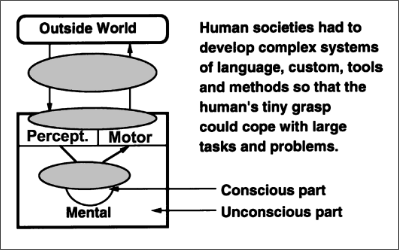
\includegraphics[scale=0.5]{images/Mondo.png}
    \caption{Visione del mondo.}
    \label{fig:Engelbart}
\end{figure}

\subsubsection{}

Per Engelbart l'addestramento è necessario per poter utilizzare i nuovi strumenti. Es. 
un aborigeno non addestrato non riuscirebbe a utilizzare una macchina, ma con il giusto addestramento composto da \fancyglitter{piccoli step}
potrebbe farlo. Infatti si impara meglio con piccoli step che con un'unica grande lezione.

\paragraph{Manipolazione simbolica:} parla dell'attività chiamata "pensiero" e di come gli esseri
umani riescano a effettuare astrazioni e \fancyglitter{manipolazione concettuale} (primo stadio di sviluppo).
Successivamente passano alla \fancyglitter{manipolazione simbolica} (secondo stadio di sviluppo) in cui si manipolano
simboli che rappresentano concetti. Il terzo stadio di sviluppo consiste nella manipolazione simbolica mediante \fancyglitter{grafici}\footnote{Questo 
è derivato dal linguaggio che si utilizza.
}. Il quarto stadio è l'unione del terzo con la componente linguistica.

\paragraph{Computazione interattiva:} Si parla della maggiore simbiosi tra uomo e macchina. Viene anche portato in evidenza il
"\fancyglitter{Bootstrap}", ossia un metodo per analizzare e migliorare il proprio lavoro in team.

\begin{figure}[h]
    \centering
    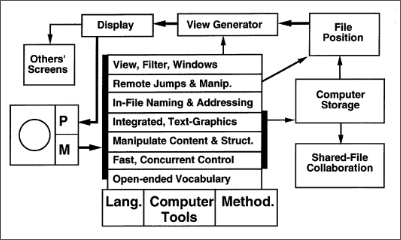
\includegraphics[scale=0.5]{images/Au.png}
    \caption{Aumentazione.}
\end{figure}

\paragraph{Supporto da ARPA:} Viene descritto il supporto che Engelbart ha ricevuto da Licklider (grazie ad ARPA) e, successivamente,
da Taylor (NASA).

\paragraph{THe Augmentation Research Center:} In questo capitolo si parla della creazione del \fancyglitter{The Augmentation Research Center} (ARC) e 
della tecnologia che è stata sviluppata al suo interno, ossia il \fancyglitter{NLS} (o \fancyglitter{oN-Line System}).
NLS è un sistema che permette di fare molte cose, tra cui la condivisione di documenti, la creazione di documenti, mail, etc.
Inoltre si parla di altri dispositivi come un oggetto che si utilizzava con una mano e aveva 5 tasti (per esempio I - insert, D - delete, etc.), ma ebbe poco successo per via dei
possibili crampi ai muscoli. Oltre a ciò veniva utilizzato un mouse analogico.

\paragraph{The Mother of All Demos (Demonstration):} Engelbart spese la maggior parte dei suoi fondi per la DEMO 
del '68, doveva essere un successo e così fu. Il capitolo si concentra su una descrizione della presentazione della DEMO.

\paragraph{Su ARPANET:} Viene descritto ARPANET (il cui secondo nodo fu ARC) e come sia stato il precursore di Internet, anche grazie a NLS.

\paragraph{Conclusione:} Si parla del declino del team di Engelbart al SRI e di come i suoi membri 
si trasferirono allo Xerox PARC. Si chiude con una considerazione riguardo al fatto che Engelbart non sia
famoso o ricco sebbene il suo lavoro abbia avuto un impatto enorme sul Web e sul concetto di personal computer.

\section{Man-computer symbiosis}

\paragraph{Introduzione:} Licklider inizia descrivendo la collaborazione tra uomo e macchina e la sua speranza che 
in futuro si possa avere una simbiosi tra i due. 

\paragraph{Scopo della simbiosi uomo-macchina:} Ci sono due scopi principali:

\begin{itemize}
    \item [$\Rightarrow$] Portare le macchine nella parte formulativa del pensiero;
    \item [$\Rightarrow$] Pensare in tempo reale.
\end{itemize}

\paragraph{Necessità della partecipazione del computer alla formulazione e 
pensare in tempo reale:} Viene descritto come l'85\% del tempo di un uomo sia speso nel 
mettersi in condizione di poter pensare, ma solo il 15\% nel pensare effettivamente.
Inoltre si parla di come il linguaggio umano sia ridondante rispetto a quello delle macchine.

\paragraph{Funzioni separabili di uomini e computer in anticipazione dell'associazione
simbiotica:} 

\begin{itemize}
    \item [$\Rightarrow$] Gli uomini si dovrebbero occupare degli obiettivi e delle ipotesi.
    Sono loro a porre i problemi e pensare a procedure e modelli. Oltre a gestire situazioni impreviste;
    \item [$\Rightarrow$] I computer si dovrebbero occupare di convertire le ipotesi in modelli 
    testabili e di testarli. Inoltre dovrebbero gestire i dettagli e le procedure. Oltre a ciò 
    i computers serviranno a fare inferenza statistica, teoria delle decisioni, teoria dei giochi, etc.
\end{itemize}

\paragraph{Prerequisiti per la realizzazione della simbiosi uomo-computer:}

\begin{itemize}
    \item [$\Rightarrow$] Differenza di velocità tra uomo e macchina: la velocità del computer 
    deve essere bilanciata con quella dell'uomo;
    \item [$\Rightarrow$] Requisiti di memoria hardware: una parte deve essere indelebile, mentre
    un'altra deve essere modificabile;
    \item [$\Rightarrow$] Requisiti di organizzazione della memoria: devono esserci specifici meccanismi
    che garantiscono l'efficienza nel recuperare informazioni;
    \item [$\Rightarrow$] Il problema del linguaggio: il computer deve essere in grado di comprendere
    un linguaggio. Per esempio il FORTRAN o l'ALGOL;
    \item [$\Rightarrow$] Equipaggiamento per l'input e l'output:
    \begin{itemize}
        \item Display e controlli;
        \item Wall display;
        \item Produzione e riconoscimento vocale.
    \end{itemize}
\end{itemize}

\section{Alan Kay's Universal Media Machine}

Si tratta del primo capitolo di un libro che parla dei principali
contributi di alcuni personaggi chiave per lo sviluppo dell'informatica.
Questo capitolo si concentra su Alan Kay.



%%%%%%%%%%%%%%%%%%%%%%%%%%%%%%%%%
% Domande
%%%%%%%%%%%%%%%%%%%%%%%%%%%%%%%%%

\definecolor{chaptergrey}{rgb}{0.5,0.5,0.5}

\ifnum\layout=2 
    \fancyhf{}      
    \renewcommand{\headrulewidth}{0pt}
    \renewcommand{\chaptermark}[1]{\markboth{#1}{}}

    \fancyhead[LE]{\nouppercase{\textbf{\textcolor{chaptergrey}{\chaptername}}~ \thechapter~ |~ \leftmark}}
    \fancyhead[RO]{\nouppercase{ \rightmark}}
    \fancyfoot[LE,RO]{\thepage}
    \fancypagestyle{plain}{         
    \fancyhf{}
    \fancyfoot[LE,RO]{\thepage}}    
 \else          
    \renewcommand{\headrulewidth}{0pt}
    \fancyhf{}                  
    \fancyhead[C]{\nouppercase{ \leftmark}}
    \fancyfoot[C]{\thepage}
\fi

\afterpage{\blankpage}
\chapter{Domande}

\section{Lullo, Leibniz e la storia del calcolo}

\qs{}{Che cos'è l'Ars Magna di Lullo?}

\paragraph{Risposta:} L'Ars Magna di Lullo è un'opera scritta da Raimondo Lullo, un filosofo, teologo e mistico catalano,
che trattava di un metodo per risolvere i problemi logici attraverso l'uso di diagrammi e figure.
In questo modo si potevano raggiungere verità in ogni campo del sapere.

\subsubsection{}

\qs{}{Quali sono le funzioni della combinatoria di Lullo?}

\paragraph{Risposta:} L'Ars Combinatoria di Lullo è un metodo inventivo
che permette di elaborare dimostrazioni allo scopo di convertire gli "infedeli" al cristianesimo\footnote{Sì, lo scopo era proprio quello.}.   

\subsubsection{}

\qs{}{Elencare almeno tre dei principi alla base della caratteristica universale di Leibniz.}

\paragraph{Risposta:}

\begin{itemize}
    \item [$\Rightarrow$] Le idee sono analizzabili;
    \item [$\Rightarrow$] L'analisi termina con le idee primitive;
    \item [$\Rightarrow$] Le idee possono essere rappresentate da simboli;
    \item [$\Rightarrow$] Le relazioni tra le idee possono essere rappresentate da simboli;
    \item [$\Rightarrow$] Le idee possono essere combinate, tramite opportune regole, per ottenere nuove idee.
\end{itemize}

\subsubsection{}

\qs{}{Elencare le principali caratteristiche della lingua universale.}

\paragraph{Risposta:}

\begin{itemize}
    \item [$\Rightarrow$] Segni che rappresentano direttamente le nozioni e le cose, non le parole;
    \item [$\Rightarrow$] Segni composti da figure geometiche e da pitture;
    \item [$\Rightarrow$] Direttamente collegata con l'enciclopedia;
    \item [$\Rightarrow$] Connessioni tra i caratteri corrispondono alle connessioni tra le cose;
    \item [$\Rightarrow$] I caratteri della lingua universale esprimono relazioni tra pensieri.
\end{itemize}

\subsubsection{}

\qs{}{Fare un esempio di proposizione dal frammento XX di Leibniz.}

\paragraph{Risposta:} Se $A \geq B$ e $B \geq C$, allora $A \geq C$.

\subsubsection{}

\qs{}{Qual è l'idea alla base di un approccio "pointless" alle nozioni geometriche e topologiche?}

\paragraph{Risposta:} L'idea alla base di un approccio "pointless" è quella che la classe
degli spazi aperti di uno spazio topologico costituisce un reticolo rispetto all'inclusione
per cui vale la proprietà di distributività.

\subsubsection{}

\qs{}{Che cosa è lo Entscheidungsproblem formulato da Hilbert e Ackermann nel 1928?}

\paragraph{Risposta:} L'Entscheidungs problem è un problema matematico che consiste nel determinare
un modo combinatorio finito per il quale combinazioni di simboli primitivi conducono a dimostrazioni.
In altre parole, trovare una procedura che consente di decidere la validità di una data
espressione logica con un numero finito di operazioni.

\section{Turing e la fisica del calcolo}

\qs{}{Perché Turing richiede che i simboli che possono essere scritti sul nastro 
di una macchina di Turing siano elementi di un insieme finito?}

\paragraph{Risposta:} Perché se l'insieme dei simboli fosse infinito, ci sarebbero un numero infinito di 
simboli molto simili tra loro, rendendo impossibile distinguerli.

\subsubsection{}

\qs{}{Perché Turing richiede che gli stati che possono essere assunti dall'unità
 di controllo di una macchina di Turing siano elementi di un insieme finito?}

\paragraph{Risposta:} Perché c'è un limite alla percezione delle caselle del nastro determinato dallo stato mentale.

\subsubsection{}

\qs{}{Che cosa stabilisce il procedimento diagonale di Cantor?}

\paragraph{Risposta:} Il procedimento diagonale di Cantor stabilisce che non esiste una corrispondenza biunivoca tra
l'insieme dei numeri naturali e l'insieme dei numeri reali. Serve a dimostrare il fatto che non tutte le funzioni 
siano calcolabili\footnote{E, per estensione, calcolabili da una macchina di Turing.}.

\subsubsection{}

\qs{}{Qual è la relazione tra una macchina di Turing generale e un automa finito?}

\paragraph{Risposta:} Un automa finito è una macchina di Turing generale con un nastro finito.

\subsubsection{}

\qs{}{Quali sono state le tappe fondamentali della formalizzazione degli automi finiti?}

\paragraph{Risposta:}

\begin{itemize}
    \item [$\Rightarrow$] Reti di neuroni di McCulloch e Pitts;
    \item [$\Rightarrow$] Eventi regolari di Kleene;
    \item [$\Rightarrow$] Lavoro di Rabin e Scott.
\end{itemize}

\subsubsection{}

\qs{}{Che cos'è il gioco della vita di Conway?}

\paragraph{Risposta:} Il gioco della vita di Conway è un automa cellulare bidimensionale (gioco a zero giocatori).
Il risultato di ogni generazione è determinato dallo stato della precedente secondo semplici regole.

\subsubsection{}

\qs{}{Qual è la relazione tra termodinamica e teoria dell'informazione?}

\paragraph{Risposta:} Von Neumann cercò di valutare il costo energetico minimo 
per un atto elementare di generazione di informazione ($kT \ln N$), ma Landauer
non riuscì a provarlo.

\subsubsection{}

\qs{}{Che cos'è il Principio di Landauer?}

\paragraph{Risposta:} Le operazioni logicamente irreversibili (cancellazione di bit) 
generano entropia pari alla quantità di informazione cancellata.

\subsubsection{}

\qs{}{Quali sono le difficoltà nell'applicazione della logica matematica classica alla formalizzazione di automi 
che descrivano sia i computer che il cervello umano?}

\paragraph{Risposta:} L'assiomatizzazione a scatole nere non è sufficiente per descrivere
il comportamento di un computer in relazione al comportamento del cervello umano.

\subsubsection{}

\qs{}{Quali sono, secondo Landauer, le operazioni che aumentano l'entropia nel processo di calcolo?}

\paragraph{Risposta:} Le operazioni che aumentano l'entropia sono quelle che comportano la cancellazione di bit.

\section{Funzioni calcolabili e combinatori}

\qs{}{Quali sono gli ingredienti principali di un sistema formale nella formulazione di Curry?}

\paragraph{Risposta:} I combinatori, la trattazione di funzioni a più argomenti
come funzioni a un solo argomento e la sostituzione.

\subsubsection{}

\qs{}{Quando una regola è ammissibile in un sistema formale?}

\paragraph{Risposta:} Una regola è ammissibile in un sistema formale se è possibile
dimostrare che essa è derivabile dalle regole di base del sistema.

\subsubsection{}

\qs{}{Indicare almeno due applicazioni dei sistemi formali alla formalizzazione di processi di riscrittura.}

\paragraph{Risposta:}

\begin{itemize}
    \item [$\Rightarrow$] Deduzione naturale di Gentzen;
    \item [$\Rightarrow$] Combinatori;
    \item [$\Rightarrow$] Lambda calcolo.
\end{itemize}

\subsubsection{}

\qs{}{Come si può caratterizzare la ricorsione strutturale?}

\paragraph{Risposta:} Con una teoria generale della sostituzione.

\subsubsection{}

\qs{}{Come può essere utilizzata la ricorsione strutturale in un linguaggio di programmazione?}

\paragraph{Risposta:} La ricorsione strutturale può essere utilizzata per definire funzioni ricorsive e tipi induttivi\footnote{Visto in "Metodi formali dell'informatica" e nella parte da +3 CFU di "Linguaggi e paradigmi di programmazione".}.

\subsubsection{}

\qs{}{Quando è opportuno usare la coricorsione per la definizione di funzioni?}

\paragraph{Risposta:} Per esempio con iteratori o generatori.

\subsubsection{}

\qs{}{Che cosa è lo schema di ricorsione primitiva?}

\paragraph{Risposta:} Lo schema di ricorsione primitiva è un metodo per definire funzioni di numeri 
naturali $f(x, n)$ a partire da funzioni predefinite $g(x)$ e $h(x, n, f(x, n))$ mediante lo schema:

$$
\begin{cases}
    f(x, 0) = g(x) \\
    f(x, n+1) = h(x, n, f(x, n))
\end{cases}
$$

\subsubsection{}

\qs{}{Che cosa è l'operatore di ricerca non limitato utilizzato da Kleene per definire le funzioni ricorsive generali?}

\paragraph{Risposta:} Dato un predicato $P(x, y)$, viene restituito il più piccolo $y$ tale che $P(x, y)$:

$$
f(x) = \mu y P(x, y)
$$

\subsubsection{}

\qs{}{Dare un esempio di almeno due combinatori con le relative uguaglianze caratteristiche.}

\paragraph{Risposta:}

\begin{itemize}
    \item [$\Rightarrow$] $K x y = x$;
    \item [$\Rightarrow$] $Y f = f (Y f)$.
    \item [$\Rightarrow$] $I x = x$;
    \item [$\Rightarrow$] $B x y z = x (y z)$;
    \item [$\Rightarrow$] $C x y z = x z y$;
    \item [$\Rightarrow$] $S x y z = x z (y z)$.
\end{itemize}

\subsubsection{}

\qs{}{Perché Curry chiamava il combinatore Y il "combinatore paradossale"?}

\paragraph{Risposta:} Perché il combinatore Y è un combinatore che si autoapplica.

\subsubsection{}

\qs{}{Come si può motivare il tipo a $\rightarrow$ (b $\rightarrow$ a) per il combinatore K? }

\paragraph{Risposta:} Prendiamo un qualsiasi x di tipo \fancyglitter{a} e un qualsiasi y di tipo \evidence{b}: 
poiché Kxy = x, il tipo di Kxy deve essere lo stesso del tipo di x, cioè \fancyglitter{a}. 
Poichè Kx prende come argomento y (un \evidence{b}) e restituisce x (un \fancyglitter{a}),
il suo tipo è y $\rightarrow$ a (ossia \evidence{b} $\rightarrow$ \fancyglitter{a}). 
Poiché K prende come argomento x (un \fancyglitter{a}) e restituisce un \evidence{b}
$\rightarrow$ \fancyglitter{a}, ha tipo \fancyglitter{a} $\rightarrow$ (\evidence{b}
$\rightarrow$ \fancyglitter{a}).

\nt{Il motivo per cui si prende sempre un argomento è perché le funzioni sono considerate
currificate.}

\qs{}{Che cosa si intende con "isomorfismo di Curry-Howard"?}

\paragraph{Risposta:} L'isomorfismo di Curry-Howard è una corrispondenza tra dimostrazioni logiche
e programmi informatici.

\section{"As we may think"}

\subsection{Sezione 1}

\qs{}{Formulare sinteticamente il complesso delle problematiche relative all'organizzazione dell'informazione.}

\paragraph{Risposta:} Si ha difficoltà nel trovare le informazioni che si stanno cercando.
Il problema deriva dal fatto che si utilizza l'indicizzazione (per nome, autore, etc.), ma 
la mente umana funziona per associazione, collegando idee tra loro.

\subsection{Sezione 6}

\qs{}{Isolare quattro problemi fondamentali delle classificazioni tradizionali (e dei relativi processi di indicizzazione).}

\paragraph{Risposta:}

\begin{itemize}
    \item [$\Rightarrow$] Artificiosità dei sistemi di indicizzazione;
    \item [$\Rightarrow$] L'informazione deve essere cercata da sottoclasse a sottoclasse;
    \item [$\Rightarrow$] Bisogna avere delle regole per localizzare le informazioni;
    \item [$\Rightarrow$] Dopo aver trovato l'elemento cercato bisogna tornare indietro.
\end{itemize}

\subsubsection{}

\qs{}{Caratterizzare l'operazione di associazione secondo Bush.}

\paragraph{Risposta:} 

\begin{itemize}
    \item [$\Rightarrow$] La mente umana scatta istantaneamente da un'idea all'altra;
    \item [$\Rightarrow$] Gli elementi non sono fissi, ma si modificano;
    \item [$\Rightarrow$] La memoria umana è associativa, ma transitoria.
\end{itemize}

\subsection{Sezione 7}

\qs{}{Elencare in modo analitico le operazioni compiute nel collegare due elementi mediante il memex. Qual è la funzione del codice e del libro dei codici?}

\paragraph{Risposta:} Un utente che crea un percorsolo nomina, lo inserisce nel libro dei codici e 
lo batte sulla sua tastiera. L'utente preme un singolo tasto e il memex collega i due elementi.
Da quel momento in poi, ogni volta che l'utente preme un elemento del percorso, il memex richiama
l'elemento collegato.

\subsubsection{}

\qs{}{Discutere la seguente affermazione: la creazione di percorsi associativi contraddice la struttura lineare del testo scritto.}

\paragraph{Risposta:} Il testo scritto è, per sua natura, immutabile, fissato in un ordine lineare. Mentre l'associazione è 
un processo dinamico, che si evolve nel tempo. Si possono creare percorsi associativi, ma il testo scritto rimane invariato.

\subsubsection{}

\qs{}{Descrivere una struttura di dati che permetta una implementazione (astratta) delle piste (trails).}

\paragraph{Risposta:} Una struttura dati che permetta di implementare le piste è un grafo. In un grafo
ogni nodo rappresenta un'idea e ogni arco rappresenta un collegamento tra due idee\footnote{Per esempio, su Obsidian (tool per MarkDown), esistono dei grafi che mostrano i collegamenti tra i propri appunti.}.

\subsubsection{}

\qs{}{Quali sono le principali operazioni di organizzazione della conoscenza compiute dall'utilizzatore del memex nell'esempio dell'arco?}

\paragraph{Risposta:} L'utente del memex, nell'esempio dell'arco:

\begin{itemize}
    \item [$\Rightarrow$] Apre un'enciclopedia, trova un articolo e lo lascia proiettato;
    \item [$\Rightarrow$] Apre un libro di storia, trova un articolo pertinente;
    \item [$\Rightarrow$] Collega i due articoli;
    \item [$\Rightarrow$] Continua a creare collegamenti;
    \item [$\Rightarrow$] Occasionalmente lascia dei commenti e aggiunge note scritte a mano da lui;
    \item [$\Rightarrow$] Diversi anni dopo e in grado di mostrare a un suo amico i percorsi che ha creato;
    \item [$\Rightarrow$] Trasferisce i percorsi sul Memex del suo amico in modo che egli possa continuare il lavoro.
\end{itemize}

\subsubsection{}

\qs{}{In quale senso le enciclopedie generate con il memex sono di un tipo totalmente nuovo?}

\paragraph{Risposta:} Sono personalizzabili e non sono statiche, ma dinamiche.

\subsubsection{}

\qs{}{In che cosa consiste la nuova professione di "apripista" (trail blazer)\footnote{Honkai Star Rail reference}?}

\paragraph{Risposta:} Gli apripista sono persone che esplorano nuovi collegamenti tra idee.
\pagebreak
\section{Engelbart e Nelson}

\subsection{Engelbart}

\qs{}{Quali sono le caratteristiche dei problemi che hanno motivato il lavoro di Engelbart sul progetto di aumentazione dell'intelligenza umana?} 

\paragraph{Risposta:} I problemi wicked.

\begin{itemize}
    \item [$\Rightarrow$] I problemi sono mal definiti;
    \item [$\Rightarrow$] Non c'è un punto in cui si possa dire che il problema è risolto;
    \item [$\Rightarrow$] Le soluzioni sono soggettive (non giuste o sbagliate);
    \item [$\Rightarrow$] Non si può procedere per tentativi;
    \item [$\Rightarrow$] Ogni problema è un caso a sé;
    \item [$\Rightarrow$] Non c'è una soluzione alterntiva preassegnata.
\end{itemize}

\subsubsection{}

\qs{}{Fare almeno due esempi di problema wicked e due esempi di problema tame.}

\paragraph{Problemi wicked:}

\begin{itemize}
    \item [$\Rightarrow$] Problemi urbanistici;
    \item [$\Rightarrow$] Organizzare una mostra.
\end{itemize}

\paragraph{Problemi tame:}

\begin{itemize}
    \item [$\Rightarrow$] Risolvere un'equazione;
    \item [$\Rightarrow$] Racimolare 10.000 euro.
\end{itemize}

\subsubsection{}

\qs{}{Che cosa intende Engelbart con "problema complesso"?}

\paragraph{Risposta:} Un problema complesso è un problema che non può essere affrontato ricorrendo a trucchetti, ma deve essere compreso.

\subsubsection{}

\qs{}{Che cosa intende Engelbart con "incremento delle capacità" (increased capability)?}

\paragraph{Risposta:} L'incremento delle capacità intellettuali umane che porti alla simbiosi
tra uomo e macchina.

\subsubsection{}

\qs{}{Che cosa intende Engelbart con "sistema H-LAM/T"? Spiegare sinteticamente ciascuno dei termini coinvolti nell'acronimo.}

\paragraph{Risposta:} Il sistema H-LAM/T\footnote{I termini sono spiegati nella sezione \ref{augmentation}.} è un sistema che permette di aumentare le capacità umane.

\begin{itemize}
    \item [$\Rightarrow$] H: Human;
    \item [$\Rightarrow$] L: Language;
    \item [$\Rightarrow$] A: Artefacts;
    \item [$\Rightarrow$] M: Methodology;
    \item [$\Rightarrow$] T: Training.
\end{itemize}

\subsubsection{}

\qs{}{In quale modo la manipolazione di simboli entra nelle considerazioni di Engelbart sulla aumentazione?}

\paragraph{Risposta:} La manipolazione di simboli è importante perché la concettualizzazione del 
mondo dipende dal linguaggio e dai simboli che si usano per rappresentare le idee.

\subsubsection{}

\qs{}{In quali aspetti il computer può contribuire come strumento di aumentazione?}

\paragraph{Risposta:} Come supporto alle operazioni e ai processi di manipolazione dei simboli.

\subsubsection{}

\qs{}{Descrivere sinteticamente di quali sono gli aspetti principali del sistema H-LAM/T che comprende un architetto aumentato.}

\paragraph{Risposta:} Un architetto aumentato:

\begin{itemize}
    \item [$\Rightarrow$] Ha già fantasticato su diverse strutture e le \fancyglitter{mette alla prova sullo schermo};
    \item [$\Rightarrow$] Sullo schermo ha una \fancyglitter{vista prospettica} del sito di costruzione sul 
    pendio della collina sormontata dalla sede stradale, rappresentazione dei vari alberi che devono rimanere
    sul terrebìno e i vari punti di allacciamento per i servizi;
    \item [$\Rightarrow$] Con il \fancyglitter{puntatore} indica due punti di interesse;
    \item [$\Rightarrow$] Dopo un po' l'architetto \fancyglitter{cambia la scena} sullo schermo in una visione dall'alto che mostra lo scavo;
    \item [$\Rightarrow$] \fancyglitter{Immette con la tastiera un elenco di elementi} controllandoli uno a uno mentre appaiono sullo schermo, rimandandone lo studio in seguito.
\end{itemize}

\subsubsection{}

\qs{}{Estendere le considerazioni di Engelbart relative a un architetto aumentato a un avvocato.}

\paragraph{Risposta:} Un avvocato aumentato:

\begin{itemize}
    \item [$\Rightarrow$] Ha già fantasticato su diverse strategie e le \fancyglitter{mette alla prova sullo schermo};
    \item [$\Rightarrow$] Sullo schermo ha una \fancyglitter{vista} del caso giudiziario sul
    quale sta lavorando, rappresentazione dei vari documenti che devono essere presentati e delle varie
    testimonianze che devono essere raccolte;
    \item [$\Rightarrow$] Con il \fancyglitter{puntatore} indica due punti articoli interessanti;
    \item [$\Rightarrow$] Si segna un elenco di casi giudiziari da studiare.
\end{itemize}

\subsubsection{}

\qs{}{Estendere le considerazioni di Engelbart relative ad un architetto aumentato ad un artista (musicista, scrittore, pittore, scultore o altro).}

\paragraph{Risposta:} Un musicista aumentato:

\begin{itemize}
    \item [$\Rightarrow$] Sullo schermo si segna un elenco di brani da studiare;
    \item [$\Rightarrow$] Con il puntatore indica gli spartiti correlati a un certo stato d'animo e li raggruppa;
    \item [$\Rightarrow$] Dopo un po' l'artista decide di confrontare due sinfonie e le fa suonare sullo schermo, mediante un dispositivo audio.
\end{itemize}

\subsubsection{}

\qs{}{Spiegare il funzionamento del sistema di schede perforate che permette una primitiva implementazione di alcune delle funzionalità del memex. Quali di queste funzionalità trovano supporto adeguato?}

\paragraph{Risposta:} Engelbart voleva utilizzare un sistema di schede perforate per ottenere delle registrazioni 
simili a quelle del memex. Le schede perforate contenevano dati, pensieri, considerazioni, concetti, idee, preocupazioni,
etc. pertinenti a un determinato argomento. Potevano facilmente essere selezionate mediante un sistema di buchi.

\subsubsection{}

\qs{}{In che senso il computer può essere considerato, per Engelbart, un medium universale?}

\paragraph{Risposta:} Il computer può essere considerato un medium universale perché può essere utilizzato per
creare, manipolare e condividere informazioni in modo flessibile. Inoltre, a differenza di altri tipi di medium,
come il libro o il cinema, con il computer si può interagire\footnote{Motivo per cui, a mio avviso, i videogiochi sono la forma d'arte più "completa".}.

\subsubsection{}

\qs{}{Illustrare brevemente gli aspetti principali degli strumenti di elaborazione dei testi presenti nel sistema nLS, come sono illustrati nella demo del 1968.}

\paragraph{Risposta:} 

\begin{itemize}
    \item [$\Rightarrow$] Il sistema nLS era concepito come una versione elettronica di una rivista scientifica;
    \item [$\Rightarrow$] Era costituito da una base di dati permanente xomposta da un insieme di documenti;
    \item [$\Rightarrow$] Era presente un sistema di indici e collegamenti incrociati;
    \item [$\Rightarrow$] Era possibile creare nuovi documenti e collegarli a quelli già presenti.
\end{itemize}

\subsubsection{}

\qs{}{Illustrare brevemente gli aspetti principali della collaborazione on-line nel sistema nLS, come sono illustrati nella demo del 1968.}

\paragraph{Risposta:}

\begin{itemize}
    \item [$\Rightarrow$] Era possibile lavorare in gruppo;
    \item [$\Rightarrow$] Gli utenti potevano inviare al journal commenti e articoli;
    \item [$\Rightarrow$] Era un "manuale della comunità";
    \item [$\Rightarrow$] Anticipava il concetto di wiki.
\end{itemize}

\subsubsection{}

\qs{}{Cenni sulla nascita dei primi modelli di personal computer allo Xerox PARC.}

\paragraph{Risposta:} Molti dei collaboratori di Engelbart si trasferirono allo Xerox PARC, dove svilupparono
il primo personal computer. Il motivo di ciò era l'idea di personal computer dello Xerox PARC, più realistica
rispetto a quella di Engelbart (il PC che rimaneva circoscritto al sistema). Fondamentali 
furono le idee di Alan Kay, che sviluppò il concetto di desktop e di finestre.

\subsection{Nelson}

\qs{}{Spiegare mediante esempi che cosa è il "testo parallelo".}

\paragraph{Risposta:} L'idea di visualizzare diversi testi contemporaneamente, in modo che l'utente possa
compararli e confrontarli tra loro. È utile per confronti, traduzioni, commenti, etc.

\subsubsection{}
\pagebreak
\qs{}{Che cosa è un ipertesto per Ted Nelson?}

\begin{figure}[h]
    \centering
    \includegraphics[scale=0.25]{images/H1.png}
    \includegraphics[scale=0.25]{images/H2.png}
    \includegraphics[scale=0.25]{images/H3.png}
\end{figure}

\qs{}{Quali sono i tipi di annotazioni (o connettori) che si possono immaginare in un ipertesto?}

\paragraph{Risposta:}

\begin{itemize}
    \item [$\Rightarrow$] Il \fancyglitter{tag}: un marcatore a cui è allegata una breve nota o spiegazione;
    \item [$\Rightarrow$] Il \fancyglitter{link}: unisce due elementi testuali. È un semplice salto da un punto all'altro.
\end{itemize}

\subsubsection{}

\qs{}{Elencare e descrivere brevemente i tipi di pista (trail) individuati da Nelson nella descrizione del memex di Bush.}

\paragraph{Risposta:}

\begin{itemize}
    \item [$\Rightarrow$] \fancyglitter{Side trails}: piste laterali che si dipartono da una pista principale;
    \item [$\Rightarrow$] \fancyglitter{Skip trails}: sottoinsiemi di una pista principale contenti i punti più importanti.
\end{itemize}

\subsubsection{}

\qs{}{In che senso, come osservato da Nelson, Bush può essere considerato l'origine della nozione di ipertesto?}

\paragraph{Risposta:} Si deve a Bush l'intuizione che la mente umana operi per associazioni.

\qs{}{Fare un esempio di ipertestualità dalla storia delle religioni, indicando esplicitamenti quali aspetti ipertestuali sono coinvolti.}

\begin{itemize}
    \item [$\Rightarrow$] \fancyglitter{Bibbia}: contiene diversi libri che si riferiscono l'uno all'altro;
    \item [$\Rightarrow$] \fancyglitter{Maha\={a}bha\={a}rata}: contiene diversi racconti che si riferiscono l'uno all'altro;
    \item [$\Rightarrow$] \fancyglitter{Talmud}: contiene diversi commenti che si riferiscono l'uno all'altro.
\end{itemize}

\subsubsection{}

\qs{}{Fare un esempio di ipertestualità dalla letteratura scientifica.}

\paragraph{Risposta:} Praticamente ogni articolo scientifico fa riferimento ad altri articoli. Per esempio in ambito matematico 
si fa riferimento a teoremi, dimostrazioni, etc.

\subsubsection{}

\qs{}{Spiegare il concetto di "collaterazione" in Nelson, facendo riferimento alle "zippered lists".}

\paragraph{Risposta:} La collaterazione è un'operazione che permette di creare una lista di elementi che si riferiscono l'uno all'altro, mediante link.
Le zippered lists sono liste che si riferiscono l'una all'altra.

\qs{}{Spiegare brevemente l'idea di "docuverso" in Nelson.}

\paragraph{Risposta:} Un docuverso è un documento che contiene un insieme di documenti che si riferiscono l'uno all'altro.

\subsubsection{}

\qs{}{Spiegare l'idea di "thinkertoy" in Computer Lib/Dream Machines di Nelson, anche commentando i suoi esempi.}

\paragraph{Risposta:} Un thinkertoy è un sistema facile e divertente da usare per aiutare le persone a pensare.
In altre parole è un sistema di visualizzazione
per computer che aiuti a considerare alternative complesse.

\subsubsection{}

\qs{}{Spiegare l'idea di "fantics" (fantica) in Computer Lib/Dream Machines di Nelson, anche commentando i suoi esempi.}

\paragraph{Risposta:} La fantics (fantica)si occupa sia delle arti espressive (scrittura, teatro e così via) sia
delle strutture e dei meccanismi del pensiero.

\begin{itemize}
    \item [$\Rightarrow$] L'arte e la scienza della presentazione;
    \item [$\Rightarrow$] Tecniche di presentazione: scrittura, regia, realizzazione di filmati, etc.
    \item [$\Rightarrow$] I media, la loro analisi, la loro progettazione, etc.;
    \item [$\Rightarrow$] La progettazione di sistemi per le presentazioni.
\end{itemize}

\section{Otlet, Lickider e Kay}

\subsection{Otlet}

\qs{}{Che cosa è il Mundaneum?}

\paragraph{Risposta:} Il Mundaneum è un'organizzazione internazionale fondata da Paul Otlet e Henri La Fontaine.
Dopo la nascita di Internet, il Mundaneum è stato rivalutato come un "Google su carta".

\subsubsection{}

\qs{}{Che cosa è la Mondothèque di Otlet?}

\paragraph{Risposta:} La Mondothèque è un'anticipazione di ciò che diventerà una workstation.

\subsubsection{}

\qs{}{Quali possibilità di trasmissione dei documenti considera Otlet nelle sue visualizzazioni?}

\paragraph{Risposta:} La videoconferenza e la didattica a distanza.

\subsubsection{}

\qs{}{Quali sono i difetti del libro secondo Otlet?}

\paragraph{Risposta:} 

\begin{itemize}
    \item [$\Rightarrow$] Non è pratico per la consultazione di specifici passaggi;
    \item [$\Rightarrow$] È un'entità completa a cui non si può aggiungere nulla;
    \item [$\Rightarrow$] Rende difficile il collegamento di elementi correlati (richiede indicizzazione).
\end{itemize}

\subsubsection{}

\qs{}{Quali sono i vantaggi delle schede realizzate secondo il Principio Monografico?}

\paragraph{Risposta:} L'utilizzo di repertorio, classificazione e ufficio della documentazione.
A ogni scheda del repertorio è associato un solo argomento. Si ha la suddivisione per contenuto informativo.

\subsection{Licklider}

\qs{}{Quali sono gli aspetti comuni tra la concezione del libro di Otlet e quella di Licklider in "Libraries of the Future"?}

\paragraph{Risposta:} Entrambi considerano il libro in veste principalmente negativa,
in quanto non permette di collegare facilmente le informazioni tra loro.

\subsubsection{}

\qs{}{Quale è stato il ruolo di Norbert Wiener nel gruppo cresciuto intorno al Research Laboratory of Electronics del MIT?}

\paragraph{Risposta:} Negli anni '30 Wiener partecipò ai seminari di Arturo Rosenblueth su metodologia e interdisciplinarità
nello studio delle comunicazioni in animali e macchine. Nel 1946 si unisce al gruppo del MIT.
Negli anni successivi partecièò alle Macy Conferences e, organizzava degli incontri il Martedì sera, in cui si 
discuteva di comunicazione come studio dei segnali secondo le leggi generali della teoria dell'informazione di Shannon.

\subsubsection{}

\qs{}{Quali sono i punti deboli nell'utilizzo interattivo del computer, prima del time-sharing?}

\paragraph{Risposta:}

\begin{itemize}
    \item [$\Rightarrow$] Il computer poteva essere utilizzato solo da un utente alla volta;
    \item [$\Rightarrow$] Il sistema precedente era batch processing;
    \item [$\Rightarrow$] Non c'era interazione in tempo reale.
\end{itemize}

\subsubsection{}

\qs{}{Quale può essere una ragionevole divisione dei compiti nella simbiosi uomo-macchina?} 

\paragraph{Risposta:} L'uomo si occupa di problemi complessi, mentre la macchina si occupa di problemi ripetitivi.

\subsubsection{}

\qs{}{Qual è la differenza principale, a livello di linguaggio, tra controllo di una macchina e controllo di un essere umano?}

\paragraph{Risposta:} Gli ordini al computer specificano \fancyglitter{procedure}, mentre gli ordini all'uomo specificano \fancyglitter{obiettivi}.

\subsubsection{}

\qs{}{Fare un esempio di feedback con un insieme di procedure predeterminato che correlano input e output.}

\paragraph{Risposta:} Vedere capitolo \ref{feedback}.

\subsubsection{}

\qs{}{Fare un esempio di feedback (interazione) in assenza di procedure predeterminate che correlano input e output.}

\paragraph{Risposta:} Vedere capitolo \ref{feedback}.

\subsubsection{}

\qs{}{Che cosa era il Memorandum for members and affiliates of the Intergalactic Computer Network di Licklider?}

\paragraph{Risposta:} Era un'idea di una rete geograficamente distribuita di utenti che condividono
risorse di calcolo, file, compilatori e programmi. Può essere considerata l'origine di ARPANET.

\subsubsection{}

\qs{}{Quali sono gli aspetti comuni alla concezione delle biblioteche adottata da Licklider in "Libraries of the Future" e la concezione di Paul Otlet?}

\paragraph{Risposta:} 


\begin{itemize}
    \item [\textcolor{red}{\XSolidBrush}] Schema della biblioteca fisica con scaffali, schede, banchi di consegna, sale di lettura;
    \item [\textcolor{red}{\XSolidBrush}] Schema del libro fisico come archivio passivo di informazione stampata;
    \item [\textcolor{red}{\XSolidBrush}] Schema della pagina stampata come strumento per la memorizzazione a lungo termine;
    \item [\textcolor{green}{\Checkmark}] Gerarchie di segmenti di testo (carattere, parola, frase, paragrafo, capitolo, libro);
    \item [\textcolor{green}{\Checkmark}] La suddivisione in informazione testuale, grafica e figurativa;
    \item [\textcolor{green}{\Checkmark}] Le parti dei documenti (indice, prefazione, appendice, bibliografia, ecc.);
    \item [\textcolor{green}{\Checkmark}] Tipologie di pubblicazioni (libri, riviste, giornali, ecc.);
    \item [\textcolor{green}{\Checkmark}] Infrastrutture come catalogo, indice, etc..
\end{itemize}

\qs{}{Indicare vantaggi e svantaggi della pagine di libro, del libro e della biblioteca}

\begin{figure}[h]
    \centering
    \includegraphics[scale=0.20]{images/Schemi.png}
\end{figure}

\qs{}{In quale senso la pagina stampata è passiva?}

\paragraph{Risposta:} La pagina stampata è passiva perché il trasferimento di informazioni richiede lo spostamento del 
lettore, del libro o di entrambi. Inoltre le operazioni di elaborazione devono essere eseguite dal lettore.

\subsubsection{}

\qs{}{Che cosa è un sistema procognitivo?}

\paragraph{Risposta:} Un sistema procognitivo è una biblioteca del futuro composta da centri di elaborazione dati
connessi tra loro.

\subsection{Alan Kay}

\qs{}{Descrivere sinteticamente il procedimento di condivisione dei file per il conputer Burroughs B220 che Alan Kay descrive come primo esempo di astrazione dei dati, nella prospettiva degli oggetti.}

\paragraph{Risposta:} 

\begin{itemize}
    \item [$\Rightarrow$] La prima parte era una \fancyglitter{sequenza di puntatori} alla seconda parte;
    \item [$\Rightarrow$] La seconda parte conteneva le \fancyglitter{procedure} utilizzate per accedere e modificare i dati della terza parte;
    \item [$\Rightarrow$] La terza parte conteneva i \fancyglitter{record} con i dati.
\end{itemize}

\subsubsection{}

\qs{}{In quale modo il funzionamento del sistema Sketchpad di Sutherland può essere confrontato con un linguaggio orientato agli oggetti?}

\paragraph{Risposta:} Kay utilizza una metafora biologica per confrontare Sketchpad con Simula 67:

\begin{itemize}
    \item [$\Rightarrow$] Le cellule ("instances") si conformano ai comportamenti "master";
    \item [$\Rightarrow$] Le cellule sono autonome e comunicano tra loro scambiandosi messaggi;
    \item [$\Rightarrow$] Le cellule diventano parti diverse di un organismo a seconda del contesto.
\end{itemize}

\subsubsection{}

\qs{}{Indicare una metafora-guida nello sviluppo delle idee di Alan Kay sugli oggetti.}

\paragraph{Risposta:} La metafora-guida è quella della biologia.

\subsubsection{}

\qs{}{In quale modo Papert ed il suo linguaggio LOGO hanno influenzato Kay?}

\paragraph{Risposta:} LOGO è un linguaggio di programmazione che permette di creare oggetti grafici.
Papert ha trasmesso a kay l'idea del computer come strumento per l'apprendimento che si 
concretizzò nel progetto Dynabook.

\qs{}{Che cosa si intende dicendo che il computer è un "medium dinamico"?}

\paragraph{Risposta:} Il computer è un medium dinamico perché permette di creare, manipolare e condividere informazioni in modo flessibile.
Non è statico come un libro o un film, ma è interattivo.

\subsubsection{}

\qs{}{In che senso il computer è un medium universale?}

\paragraph{Risposta:} Il computer è un medium universale perché può simulare 
qualsiasi altro medium.



\end{document}